\documentclass{mybook}
\usepackage[T2A]{fontenc}
\usepackage[utf8]{inputenc}
\usepackage[english,russian]{babel}

\usepackage{amsthm}
\usepackage{graphicx}
\usepackage{wrapfig}
\usepackage{amssymb}
\usepackage{amsmath}
\usepackage{graphicx}
\usepackage{subfig}
\usepackage{color}
\usepackage{bm}
\usepackage{tabularx}
\usepackage{url}
\usepackage{multirow}
\usepackage{lastpage}
 \usepackage{systeme}

\usepackage[toc,page]{appendix}
\usepackage{hyperref}

\usepackage{geometry}
\geometry{left=1.5cm}
\geometry{right=1.5cm}
\geometry{top=2.0cm}
\geometry{bottom=3.0cm}
\renewcommand{\baselinestretch}{1.0}

%https://tex.stackexchange.com/questions/163451/total-number-of-citations
\usepackage{totcount}
\newtotcounter{citnum} %From the package documentation
\def\oldbibitem{} \let\oldbibitem=\bibitem
\def\bibitem{\stepcounter{citnum}\oldbibitem}

\makeatletter
\long\def\@makecaption#1#2{%
  \vskip\abovecaptionskip
  \sbox\@tempboxa{#1.~#2}%
  \ifdim \wd\@tempboxa >\hsize
    #1.~#2\par
  \else
    \global \@minipagefalse
    \hb@xt@\hsize{\hfil\box\@tempboxa\hfil}%
  \fi
  \vskip\belowcaptionskip}
\makeatother

\reversemarginpar

\usepackage[
backend=biber,
style=numeric,
sorting=ynt
]{biblatex}
\addbibresource{chapters/*/main.bib}

\begin{document}
% Титульный лист
\thispagestyle{empty}

\vspace{3cm}
  \begin{center}
	\bfseries \Huge Интеллектуальные системы  \par   % Your own title would go here.
        ~\\
	\bfseries \LARGE Кафедра Интеллектуальных Систум \\   % Include a subtitle or just delete.
    \end{center}

\setcounter{page}{2}

% Оглавление
\newpage
\tableofcontents
    
    % Example chapter
    \clearpage
    \chapter{Пример Отчета}
    \section{Introduction}

Each report must be created in a separate subfolder. Take the "example" folder as an example of a report (please do not change).

All changes are made through GitHub\footnote{\url{https://github.com/Intelligent-Systems-Phystech/IntelligentSystem}}. It is recommended to create a new project in overleaf by using <<Import from GitHub>> utility. And after all changes push it back to GitHub by using <<Menu -> Sync -> GitHub>>.

As an example, consider a linear regression problem.


After writing your report, include the report to main.tex similar to the sample report.

\section{References Review}

Here, please write a short description of each paper in your reference list.

It is important to indicate a list of references on this topic~\cite{AuthorYear}. All references put to the main.bib file.


\section{Main Part}

This section describes the topic that will be discussed in the seminar.

\section{Questions To Discussion}
List of questions to be discussed at the seminar.
\begin{enumerate}
    \item First question.
    \item Second question.
    \item ...
\end{enumerate}
    
    % Other chapters
    \clearpage
    \chapter{Continuous-Time Representation and Legendre Memory Units for BCI}
    \newcommand{\vect}[1]{\textbf{#1}}

\section{Introduction}

Рассматривается задача декодирования сигналов активности головного мозга и построения нейроинтерфейса, работающего с временными рядами как с непрерывными во времени. В качестве решения предлается использовать рекуррентные модели с модифицированным скрытым состоянием, которое определяется как решение обыкновенного дифференциального уравнения. Считается, что такой подход позволит повысить производительность обработки нерегулярных временных рядов, которые возникают при непостоянном контакте со считывающим устройством, а так же будет применим для передискретизации сигнала при низких частотах сэмплирования, поскольку доступные для широкого круга устройства обычно имеют невысокую частоту дискретизации. Кроме этого ожидается получение непрерывного представления сигнала для возможного дальнейшего использования в качестве признакового описания.  

Обычно нейроинтерфейс предполагает работу с данными многомерных временных рядов (сигналов активности головного мозга). Наиболее распространенными для регистрации сигналов являются неинвазивные методы на основе электроэнцефалографии, не требующие операции для установки датчиков, обладающие низкой стоимостью, высоким временными разрешением и простотой в настройке. 
\begin{figure}[!h]
	\centering
	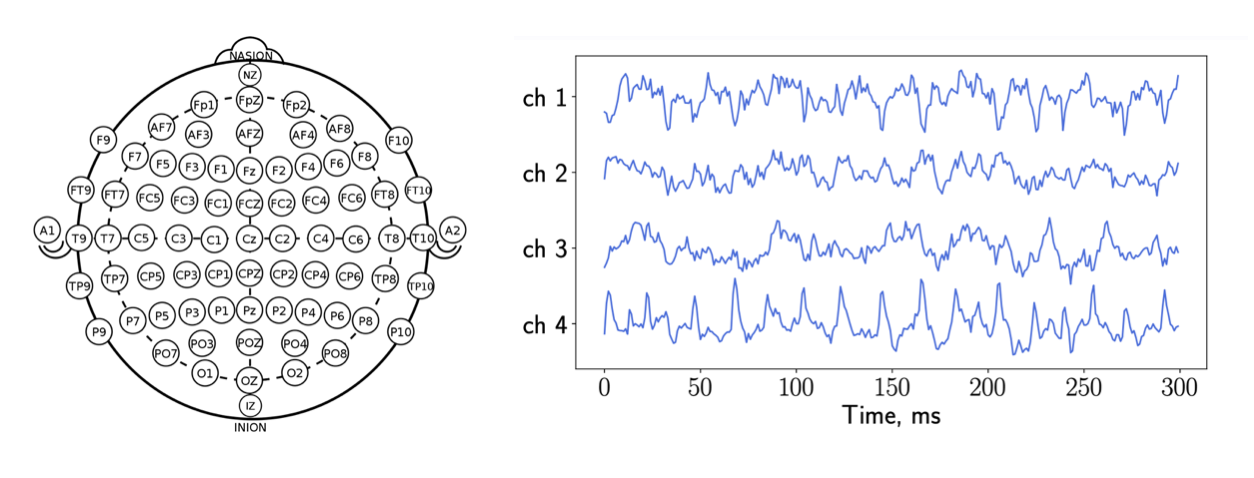
\includegraphics[width=0.8\textwidth]{chapters/varenik1/electodes-signal.png}
\end{figure}

При непрерывном представлении сигнала предполагается, что у нас есть некий процесс $V(t)$ - активность мозга и его реализация $\vect x_{t_i} \approx V(t_i)$ - наблюдаемый сигнал. Требуется построить функцию $f_{\vect X}(t): \mathbb{R}\to \mathbb{R}^E$, которая для любого момента времени сможет предоставить некоторое приближение сигнала или процесса $f_{\vect X}(t) \approx \vect x_t \approx V(t)$.

\textit{\textbf{Гипотеза.}}
Предлагается использовать скрытое состояние нейронных ОДУ (Neural ODE) в качестве непрерывныго представления сигнала.

\textit{\textbf{Критерии.}}
Скрытое состояние является непрерывным представлением сигнала, если оно удволетворяет следующим требованиям:
\begin{itemize}
    \item можно извлечь из модели и использовать самостоятельно как представление сигнала,
    \item сохраняет форму приближаемого процесса,
    \item позволяет получить значение в произвольный момент времени.
\end{itemize}
\section{References Review}
Статья~\cite{NEURIPS2018_69386f6b} является основной по теме Neural ODE. Вдохновившись синтаксической схожестью преобразования скрытого состояния в сети ResNet с формулой Эйлера для численного интегрирования ОДУ авторы предлагают механизм обратного распространения ошибки для обучения непрерывного в глубину аналога ResNet со скрытым состоянием, подчиняющимся ОДУ с параметризованной функцией динамики, параметры которой находятся минимизацией функции ошибки. В~\cite{NEURIPS2019_42a6845a} рассматривается ODE-модификация RNN для работы с нерегулярными по времени временными рядами. Идея состоит в доопределении скрытого состояния между наблюдениями решением нейронного ОДУ и корректировки полученной динамики в точках наблюдений по стандартному принципу RNN. Такое неявное добавление времени в состояние модели позволяет учесть информацию о временном интервале между наблюдениями, которая может быть полезна при обработке нерегулярных данных. Работа~\cite{DBLP:journals/corr/abs-2005-08926} посвящена еще одной модификации RNN для работы с данными, имеющими непостоянный шаг по временной шкале. В ней предлагается моделировать скрытое состояние управляемым дифференциальным уравнением, что позволяет получить непрерывную по отношению к входным наблюдениям функцию скрытого состояния. Для обработки длинных последовательностей нерегулярных временных рядов также имеются непрерывные по времени обобщения LSTM: в~\cite{DBLP:journals/corr/abs-2006-04418} рассматривается подход аналогичный ODE-RNN и показано, что предложенная архитектура аналогично стандартной не страдает от взрыва и затухания градиентов. В основе ~\cite{NEURIPS2019_952285b9} лежит построение ячейки памяти, представляющей непрерывное представление истории изменения сигнала в виде разложения на полиномы Лежандра, где в качестве коэффициентов используется компоненты состояния памяти LMU-LSTM.
\section{Main Part}

\textit{\textbf{Neural ODE.}}

Пусть задан процесс, который подчиняется некоторому неизвестному ОДУ и пусть известны несколько наблюдений вдоль траектории процесса, для простоты будем считать что их $2: t_0, t_1$ - в начале и в конце траектории:
\begin{equation}
    \frac{d\vect z}{dt} = f(\vect z(t), t), \{(\vect z_0, t_0), (\vect z_1, t_1)\} - \text{наблюдения}.
\end{equation}

Нужно найти аппроксимацию функции динамики $f(\vect z(t), t, \theta)$. 
В качестве аппроксиманта выступает нейронная сеть с параметрами $\theta$. Эволюция системы запускается из начального состояния на время $t_1 - t_0$ с какой-то параметризованной функцией динамики используя любой метод эволюции ОДУ. После того как система окажется в новом состоянии $\hat{\vect z}_1$ оно сравнивается с истинным  $\vect z_1$ и разница минимизируется поиском оптимальных параметров методом обратного распространения ошибки:
\begin{equation}
    L(\vect z(t_1)) = L(\vect z(t_0) + \int\limits_{t_0}^{t_1} f(\vect z(t), t, \theta))dt = L(ODESolver(\vect z(t_0), f, t_0, t_1, \theta)).
\end{equation}

Чтобы минимизировать $L$ нужно уметь эффективно проводить непрерывный по времени backpropagation. Для начала определим, как градиент функции потерь зависит от скрытого состояния:
\begin{equation}
    \vect a(t) = \frac{\partial L}{\partial \vect z(t)},
\end{equation}
эта величина называется сопряженным состоянием. Его динамика задается другим ОДУ:
\begin{equation}
    \frac{d\vect a(t)}{dt} = -\vect a(t)^T\frac{\partial f(\vect z(t), t, \theta)}{\partial \vect z},
\end{equation}
\begin{equation}
    \vect a(t_0) = \vect a(t_1) - \int\limits_{t_1}^{t_0} \vect a(t)^T\frac{\partial f(\vect z(t), t, \theta)}{\partial \vect z} \text{ при } \vect a(t_1) = \frac{dL}{d\vect z(t_1)}.
    \label{eq1}
\end{equation}

В общем случае нужно найти градиенты по всем входным параметрам решателя ОДУ. Рассмотрим как найти градиенты по $\vect z_0$ и $\theta$ за один проход. 

Для этого вводится аугментированное состояние - обычное состояние $\vect z$ к которому добавили $\theta$. Его динамика тривиальным образом определяется из оригинальной динамики:
\begin{equation}
    \frac{d}{dt}\begin{bmatrix}
        \vect z \\
        \theta \\
        \end{bmatrix}(t) = f_{aug}([\vect z, \theta]) := \begin{bmatrix}
        f([\vect z, \theta, t]) \\
        \vect 0 \\
    \end{bmatrix},
\end{equation}

сопряженное состояние к такому аугментированному:
\begin{equation}
    \vect a_{aug} := \begin{bmatrix}
    \vect a \\
    \vect a_{\theta} \\
    \end{bmatrix},
    \vect a_{\theta} := \frac{dL}{d\theta(t)}.
\end{equation}

Посчитав градиент аугментированной динамики:
\begin{equation}
    \frac{\partial f_{aug}}{\partial [\vect z, \theta]} =  \begin{bmatrix}
    \frac{\partial f}{\partial \vect z}&\frac{\partial f}{\partial \theta}\\
    \vect 0&\vect 0\\
    \end{bmatrix}(t),
\end{equation}
получим дифференциальное уравнение для аугментированного сопряженного состояния:
\begin{equation}
    \frac{d\vect a_{aug}(t)}{dt} = \begin{bmatrix}
    \vect a(t) & \vect a_{\theta}(t)
    \end{bmatrix} \frac{\partial f_{aug}}{\partial [\vect z, \theta]}(t) = - \begin{bmatrix}
    \vect a(t)\frac{\partial f}{\partial \vect z} & \vect a(t)\frac{\partial f}{\partial \theta}
    \end{bmatrix}.
\end{equation}

Исходя из полученной динамики мы легко можем определить градиент по $\theta$ как решение ДУ назад во времени для $\theta$-компоненты:
\begin{equation}
    \frac{dL}{d\theta} = \vect a_{\theta}(t_0) =  - \int\limits_{t_1}^{t_0}\vect a(t)^T\frac{\partial f(\vect z(t), t, \theta)}{\partial \theta}dt \text{ при } \vect a_{\theta}(t_1) = \vect 0.
    \label{eq2}
\end{equation}

Градиент по $t$ можно найди аналогичным образом добавив его в аугментированное состояние. Таким образом, чтобы получить требуемые градиенты нужно вычислить \ref{eq1} и \ref{eq2} назад во времени начиная с $t_1$.

Все необходимые градиенты можно получить за один проход алгоритма непрерывного обратного распространения с использованием решения аугментированного ДУ:

\begin{figure}[!h]
	\centering
	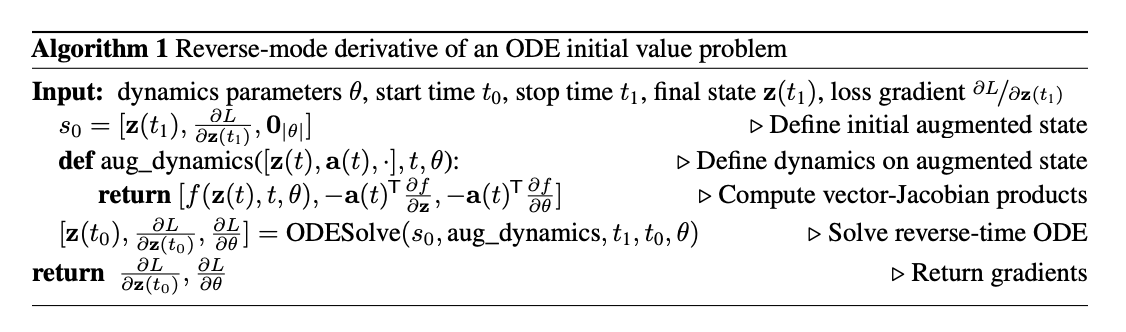
\includegraphics[width=0.9\textwidth]{chapters/varenik1/backpropagation-algo.png}
\end{figure}

Ввиду того, что вычисление рассмотренных двух интегралов требует знания $\vect z(t)$ на всей траектории и с учетом того, что решатель ОДУ может выводить значения состояния для некоторого набора отсчетов времени предлагается запускать эволюцию состояния $\vect z(t)$ вместе с сопряженным состоянием назад во времени. Тогда распространение назад сопряженного состояния разбивается на части и проводится корректировка в точках наблюдений в направлении соответствующих градиентов (см. рис. \ref{fig:im1}).

\begin{figure}[!h]
	\centering
	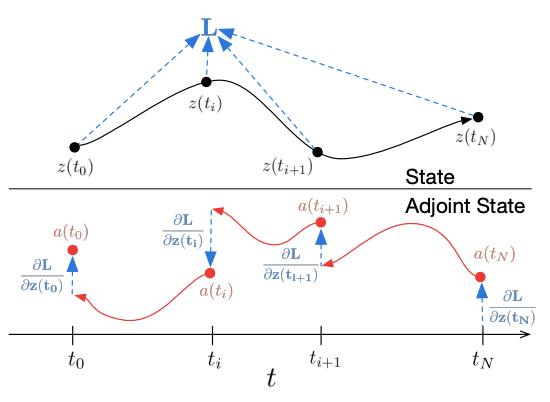
\includegraphics[width=0.45\textwidth]{chapters/varenik1/backpropagation.png}
	\caption{Непрерывное распространение назад.}
	\label{fig:im1}
\end{figure}

\newpage
\textit{\textbf{ODE-RNN.}}

Рассмотрим нерегулярный временной ряд:
\begin{equation*}
    \vect X = \{(\vect x_i, t_i)\}_{i=0}^N, t_i\in \mathbb{R}, t_0 \le \dots \le t_N, \Delta_t = t_{i+1} - t_{i} \neq const, \vect x_i \in \mathbb{R}^E
\end{equation*}

\begin{wrapfigure}{r}[8pt]{.45\textwidth}
    \centering
    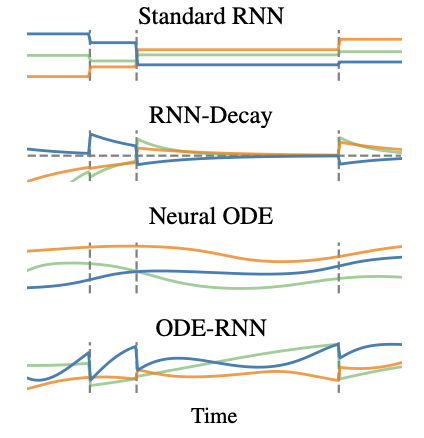
\includegraphics[scale=0.9]{chapters/varenik1/ode-rnn.png}
    \caption{Динамика скрытых состояний разных размерностей. Вертикальные линии соответствуют временам наблюдений.}
\end{wrapfigure}

Самым распространенным подходом для анализа регулярных последовательностей являются рекуррентные модели. Но они в своем построении предполагают равномерный одинаковый шаг между наблюдениями, и таким образом не способны извлекать информацию о времени измерения, которая может быть полезна в качестве описания при анализе нерегулярных данных. Следовательно, нужно определить зависимость состояния от расстояния во времени между наблюдениями. Естественным в таком случае кажется введение модели с непрерывным скрытым состоянием. 

Один из простых вариантов учета дельты - добавить ее в качестве входной переменной в ячейку RNN, но тогда остается открытым вопрос как определить состояние между моментами наблюдений:
\begin{equation*}
    \vect h_i = RNNCell(\vect h_{i-1}, \Delta_t, \vect x_i), \text{ }\Delta_t = t_i - t_{i-1};
\end{equation*}

Следующее решение - определить динамику между наблюдениями через экспоненциальный спад:
\begin{equation*}
    \vect h_i = RNNCell(\vect h_{i-1} \exp(-\tau \Delta_t), \vect x_i), \text{ } \tau - \text{параметр спада};
\end{equation*}

Однако, экспериментально было показано, что такая модификация не дает улучшения в производительности по сравнению со стандартной архитектурой. Поэтому, предлагается вводить непрерывную во времени динамику через решение  Neural ODE: 
\begin{equation*}
    \vect h_0, \dots, \vect h_N = ODESolver(f_{\theta}, \vect h_0, (t_0, \dots, t_N));
\end{equation*}

Обычный подход ODE хоть и задает сложную траекторию скрытого состояния, но она определяется лишь начальным состоянием и не адаптируется к поступающим наблюдениям. Следовательно, предлагается модификация преобразования состояния в рекуррентной сети, в которой состояние между наблюдениями определяется как решение ODE, а в точках наблюдений происходит обновление, аналогичное стандартной RNN:
\begin{align*}
   & \vect h_i' = ODESolver(f_{\theta}, \vect h_{i-1}, (t_{i-1}, t_i)),\\
   & \vect h_i = RNNCell(\vect h_i', \vect x_i).
\end{align*}

\textit{\textbf{Neural CDE.}}

Рассмотрим другое расширение обычных нейронных уравнений, способное предоставить непрерывное представление сигнала, учитывающее входящие наблюдения, которые могут быть как нерегулярными, так и частично наблюдаемыми - нейронные управляемые уравнения.

Пусть $S:[t_0, t_N] \to \mathbb{R}^{E+1}$ - натуральный кубический сплайн с узлами в $t_0, \dots, t_N$, $S_{t_i} = (\vect x_i, t_i)$, который по построению является аппроксимацией процесса с реализациями, представленными в $\vect X$. 

Пусть $f_{\theta}: \mathbb{R}^d \to \mathbb{R}^{d\times (E+1)}$, $g_{\theta}: \mathbb{R}^{E+1} \to \mathbb{R}^{d}$ - нейронные сети, зависящие от параметра $\theta$, $d$ - размерность скрытого пространства.

Тогда скрытое состояние определяется, как решение управляемого ДУ:
\begin{equation}
   \vect z_t = \vect z_{t_o} + \int\limits_{t_0}^t f_{\theta}(\vect z_{\tau})dS_{\tau}, t\in (t_0, t_N], \text{ где } \vect z_{t_0} = g_{\theta}(\vect x_0, t_0).
\end{equation}

\begin{figure}[!h]
	\centering
	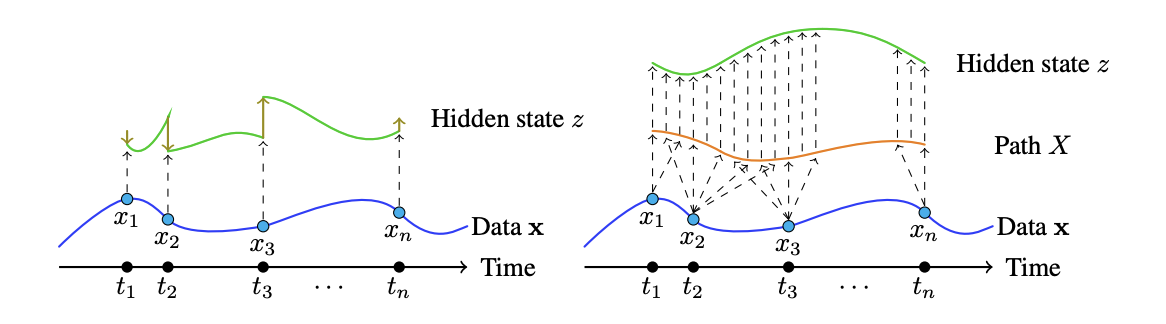
\includegraphics[width=0.8\textwidth]{chapters/varenik1/neural-cde.png}
	\caption{Сравнение скрытого состояния ODE-RNN и Neural CDE.}
	\label{fig:im2}
\end{figure}

По своей архитектуре рассмотренный подход также является рекуррентной моделью, но главное отличие от предыдущей архитектуры состоит в непрерывности скрытого состояния по отношению к наблюдениям см. рис. \ref{fig:im2}).

\textit{\textbf{ODE-LSTM.}}

Ввиду известной проблемы взрыва и затухания градиентов для RNN, их применение становится невозможным для обработки длинных последовательностей. Общепринятым решением является модель LSTM. 

Скрытое состояние - пара $(\vect c_t, \vect h_t)$, $\vect c_t$ - состояние долгосрочной памяти, $\vect h_t$ - обычное скрытое состояние.

Функция обновления $f_{\theta}(\vect x_{t+1}, (\vect c_t, \vect h_t)) \mapsto (\vect c_{t+1}, \vect h_{t+1})$ определяется набором уравнений:
\begin{align*}
    & \vect z_{t+1} = tanh(\vect W_z \vect x_{t+1} + \vect R_z\vect h_t+\vect b_z),\\
    & \vect i_{t+1} = \sigma(\vect W_i\vect x_{t+1} + \vect R_i \vect h_t + \vect b_i),\\
    & \vect f_{t+1} = \sigma(\vect W_f\vect x_{t+1} + \vect R_f \vect h_t + \vect b_f + \vect 1),\\
    & \vect o_{t+1} = \sigma(\vect W_o\vect x_{t+1} + \vect R_o \vect h_t + \vect b_o),\\
    & \vect c_{t+1} = \vect z_{t+1}\odot \vect i_{t+1} + \vect c_t\odot \vect f_{t+1},\\
    & \vect h_{t+1} = tanh(\vect c_{t+1})\odot \vect o_{t+1}.
\end{align*}

Аналогично RNN производится ODE модификация LSTM, предоставляющая непрерывный учет времени в скрытом состоянии:
\begin{align*}
    & (\vect c_{t+1}, \vect h_{t+1}') = LSTM(\theta_l, (\vect c_t, \vect h_t), \vect x_{t+1})),\\
    & \vect h_{t+1} = ODESolver(f_{\theta}, \vect h_{t+1}', t_{t+1} - t_{t}),\\
    & \vect o_{t+1} = \vect h_{t+1}\vect W_{output} + b_{output}.
\end{align*}

\textit{\textbf{LMU-LSTM}}

Рассмотрим еще одну модификацию LSTM - Legendre Memory Units. Главным компонентом является ячейка памяти, описываемая системой d связанных ОДУ:
\begin{equation*}
    \theta \dot{\vect c(t)} = \vect A\vect c(t) + \vect bu(t),
\end{equation*}
где $\vect c(t)\in \mathbb{R}^d$ - состояние долгосрочной памяти,
$u_t \in \mathbb{R}$ - история изменения входящего сигнала.

Наилучшие матрицы $(\vect A, \vect b)$ получаются с помощью аппроксимантов Паде:

\begin{center}
    $\vect A = [a]_{ij} \in \mathbb{R}^{d\times d}, \text{ } a_{ij} = (2i+1)
    \begin{cases}
        -1 & i < j \\
        (-1)^{i-j+1} & i\ge j\\
    \end{cases}$,
\end{center}
\begin{center}
    $\vect b = [b]_i \in \mathbb{R}^{d\times 1},  \text{ } b_i = (2i+1)(-1)^i,  \text{ } i, j \in [0, d-1]$.
\end{center}

Основное свойство данной динамической системы заключается в том, что $\vect c(t)$ представляет скользящее окно $u$ по полиномам Лежандра степени до $d-1$:

\begin{equation*}
    u(t-\theta') \approx \sum\limits_{i=0}^{d-1} \mathcal{P}_i\Bigg(\frac{\theta'}{\theta}\Bigg)c_i(t), \text{ } 0\le \theta' \le \theta, \text{ } \mathcal{P}_i(r) = (-1)^i\sum\limits_{j=0}^i\binom{i}{j}\binom{i+j}{j}(-r)^j
\end{equation*}

где $\mathcal{P}_i(r)$ - сдвинутые полиномы Лежандра.
\begin{figure}[!h]
	\centering
	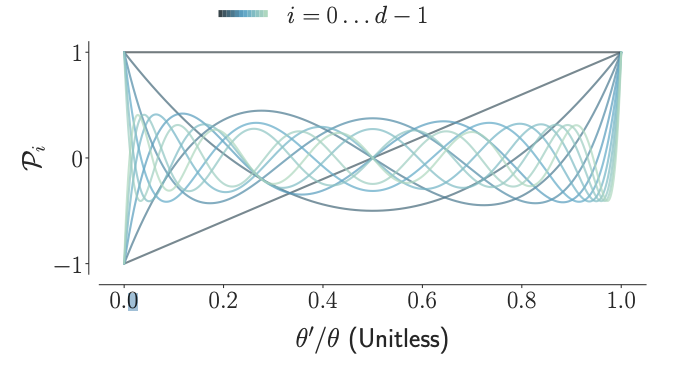
\includegraphics[width=0.55\textwidth]{chapters/varenik1/legendre.png}
\end{figure}

\textit{\textbf{Применение к декодированию \footnote{\url{http://www.machinelearning.ru/wiki/images/6/62/Samokhina2021MSThesis.pdf}}}}

Здесь приведены результаты работы Алины по построению непрерывного представления. Построение осуществлялось в рамках решения задачи классификации потенциалов $P300$, где непрерывное представление извлекалось из скрытого состояния алгоритмов классификации. $P300$ это потенциал активности мозга, в котором пик соответствует реакции на внешний стимул. 

Было показано, что скрытое состояние Neural CDE отвечает всем поставленным критериям непрерывного представления сигнала. Состояние $z(t)$ не является точным описанием процесса $V(t)$, но сохраняет его форму.
	
\begin{figure}[ht]%
    \centering
    \subfloat[Потенциал P300.]{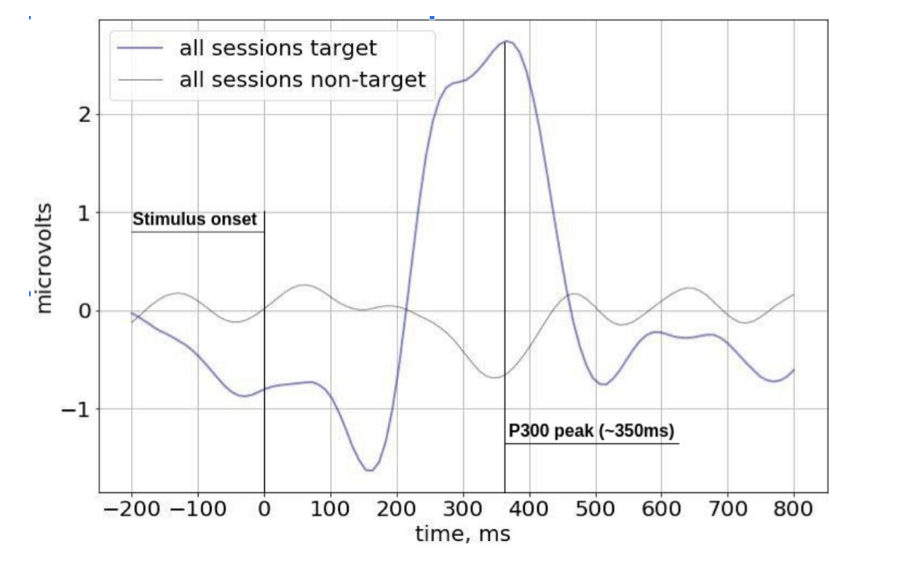
\includegraphics[width=0.47\linewidth]{chapters/varenik1/p300.png}}\qquad
    \subfloat[Непрерывное представление сигнала.]{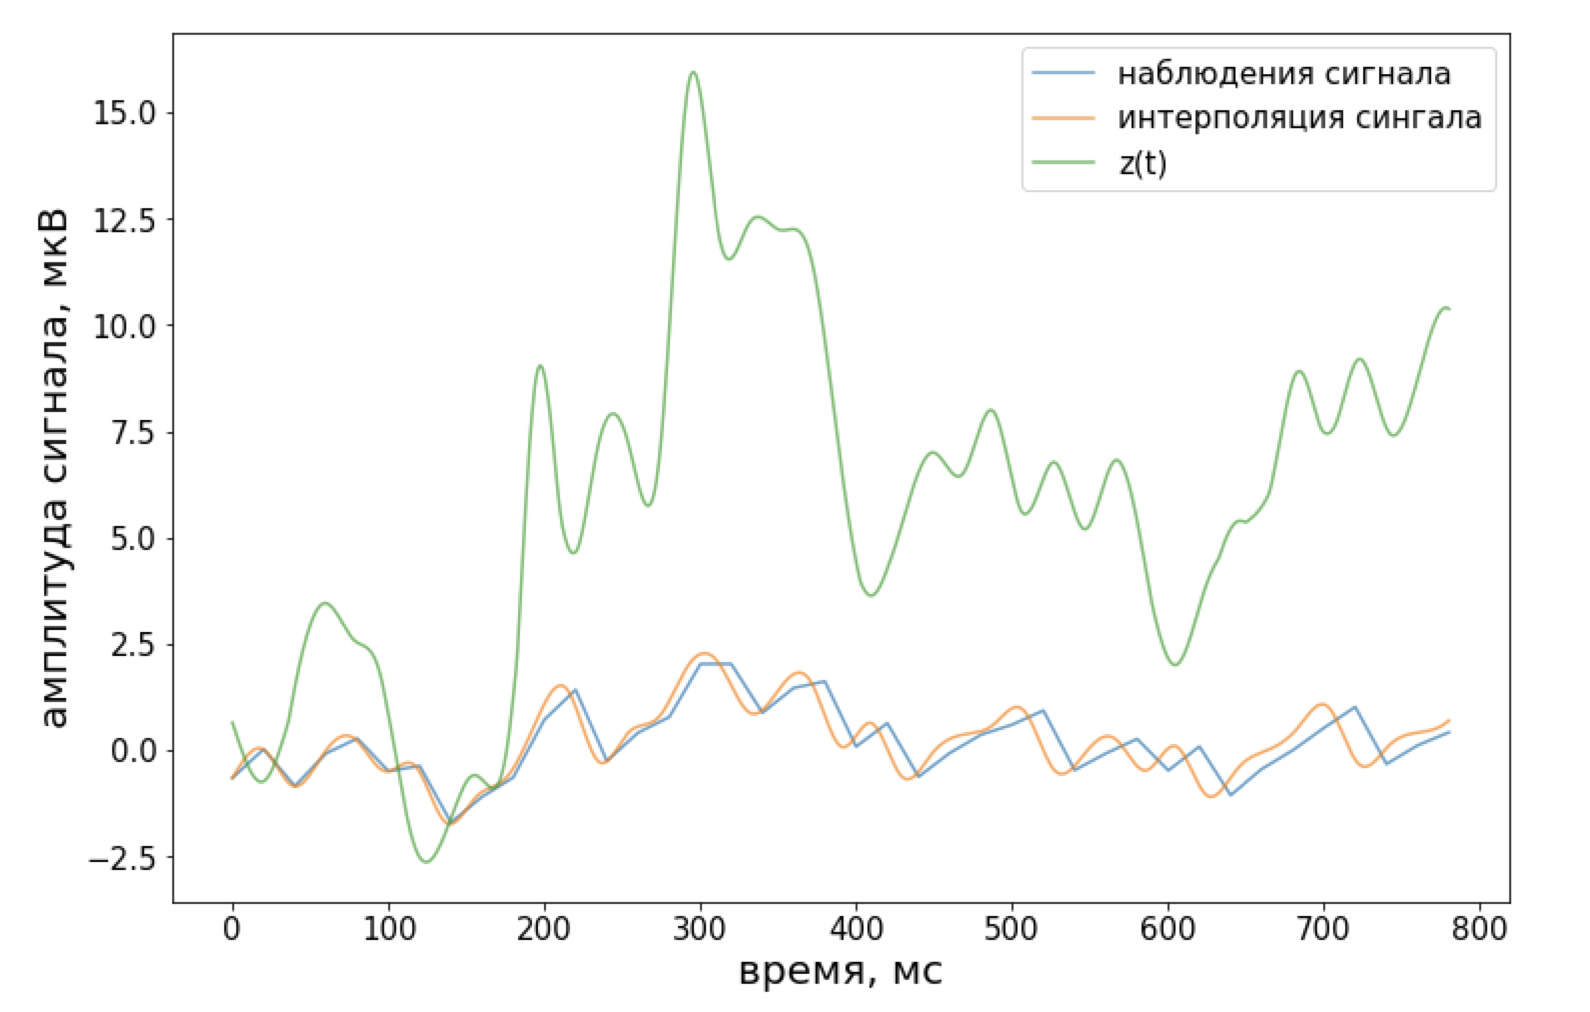
\includegraphics[width=0.46\linewidth]{chapters/varenik1/result.png}}
\end{figure}

\section{Questions To Discussion}
\begin{enumerate}
    \item Для чего нужно непрерывное по времени представление сигнала.
    \item Как работает непрерывный метод обратного распространения ошибки.
    \item Почему стандартная RNN не подходит для анализа нерегулярных временных рядов.
    \item В чем преимущество Neural CDE над ODE-RNN.
\end{enumerate}

    \clearpage
    \chapter{Rectangular flows}
    \newcommand{\bh}{\mathbf{h}} 
\newcommand{\bt}{\mathbf{t}} 
\newcommand{\bu}{\mathbf{u}} 
\newcommand{\bv}{\mathbf{v}} 
\newcommand{\bw}{\mathbf{w}} 
\newcommand{\bx}{\mathbf{x}} 
\newcommand{\bz}{\mathbf{z}} 
\newcommand{\by}{\mathbf{y}} 

\newcommand{\bA}{\mathbf{A}} 
\newcommand{\bC}{\mathbf{C}} 
\newcommand{\bI}{\mathbf{I}} 
\newcommand{\bT}{\mathbf{T}} 
\newcommand{\bW}{\mathbf{W}} 
\newcommand{\bX}{\mathbf{X}} 
\newcommand{\bZ}{\mathbf{Z}} 

\newcommand{\bepsilon}{\boldsymbol{\epsilon}}
\newcommand{\bmu}{\boldsymbol{\mu}}
\newcommand{\blambda}{\boldsymbol{\lambda}}
\newcommand{\bsigma}{\boldsymbol{\sigma}}
\newcommand{\bSigma}{\boldsymbol{\Sigma}}

\newcommand{\bbE}{\mathbb{E}} 
\newcommand{\bbP}{\mathbb{P}} 
\newcommand{\bbQ}{\mathbb{Q}} 
\newcommand{\bbR}{\mathbb{R}} 

\newcommand{\mbbP}{\mathbb{P}_{\text{MCMC}}}

\newcommand{\cL}{\mathcal{L}} 
\newcommand{\cN}{\mathcal{N}} 
\newcommand{\cS}{\mathcal{S}} 
\newcommand{\cT}{\mathcal{T}} 
\newcommand{\cX}{\mathcal{X}} 
\newcommand{\cB}{\mathcal{B}}
\newcommand{\cY}{\mathcal{Y}}
\newcommand{\cP}{\mathcal{P}}
\newcommand{\cF}{\mathcal{F}}
\newcommand{\cW}{\mathcal{W}}
\newcommand{\cE}{\mathcal{E}}
\newcommand{\cU}{\mathcal{U}}
\newcommand{\cV}{\mathcal{V}}
\newcommand{\cM}{\mathcal{M}} 

\newcommand\footfullcitenonum[1]{%
  \begingroup
  \renewcommand\thefootnote{}\footfullcite{#1}%
  \addtocounter{footnote}{-1}%
  \endgroup
}

\newcommand\footnotenonum[1]{%
  \begingroup
  \renewcommand\thefootnote{}\footnote{#1}%
  \addtocounter{footnote}{-1}%
  \endgroup
}

\definecolor{mgreen}{RGB}{0, 170, 0}

\newcommand{\green}[1]{{\color{mgreen} #1}}
\newcommand{\red}[1]{{\color{red} #1}}
\definecolor{myellow}{RGB}{255, 204, 0}
\newcommand{\yellow}[1]{{\color{myellow} #1}}

\definecolor{mysunset}{RGB}{255, 143, 1}
\newcommand{\sunset}[1]{{\color{mysunset} #1}}

\definecolor{mytwilight}{RGB}{29, 55, 176}
\newcommand{\twilight}[1]{{\color{mytwilight} #1}}

\newcommand{\bbRn}{\mathbb{R}^n}
% \newcommand{\bbR}{\mathbb{R}}
% \newcommand{\bbP}{\mathbb{P}} 

\section{Introduction}

В некоторых практических приложениях исследуемые данные лежат на на некотором многообразии $\cM^n \cong \bbR^n$ вложенного в $\bbR^N$, $n < N$. Необходимо построить модель машинного обучения, способную семлировать данные из целевого распределения/оценивать плотность целевого распределения. В качестве моделей рассматриваются потоковые структуры (то есть модели, обучающиеся с помощью метода максимизации правдоподобия и, как правило, обратимые)

\begin{figure}[!h]
\vspace{-5mm}
	    \centering
	  \vspace{2mm}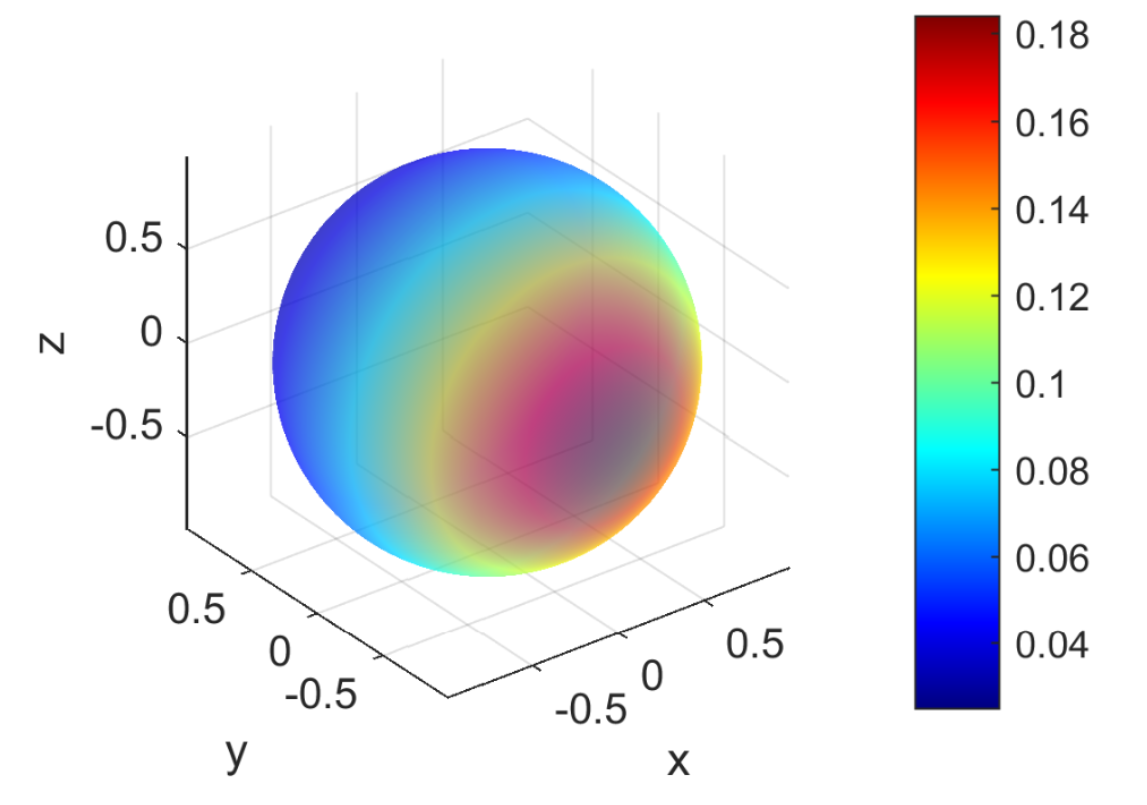
\includegraphics[width=0.5\linewidth]{chapters/petr_mokrov_s1/figs/VonMisesSphere.png}
	    \caption{{Пример von Mises-Fisher распр. на $S^2$}}
\end{figure}

\section{References Review}
\begin{itemize}
    \item \cite{dinh2017density} : В этой статье предлагается RealNVP - классическая Normalizing Flow модель.
    
    \item \cite{gemici2016normalizing} : Normalizing flows на многообразии, в предположении, что многообразие (карта) известна.
    
    \item \cite{beitler2019pie} : В этой статье предлагается PIE (Pseudo-Invertible Encoder) - одна из первых моделей, которая может учит многообразие и распределение на нём.
    
    \item \cite{NEURIPS2020_05192834} : Основная статья доклада, в ней предлагается $\cM$ и $\cM_e$ - потоки, явно учат целевое многообразие и честно оценивают плотность на нём, обучение двухстадийное (чередуются обучение карты и максимизация правдоподобия) что позволяет избежать оценки сложновычислимого якобиана карты.
    
    \item \cite{caterini2021rectangular} : Современный подход для обучения Rectangular flows на многообразии, при обучении с помощью различных технических процедур удаётся оценивать якобиан карты и производить оптимизацию исключительно максимизируя правдоподобие
\end{itemize}

\section{Main Part}

\subsection{Normalizing flows}

Напомним устройство классических нормализующих потоков. Имеется $x$ - целевая случайная величина, для латентной переменной $z$ фиксируется распределение. Строится $f: \bbR^N \rightarrow \bbR^N$ - диффеоморфизм. Формулы замены переменной: $p(x) = p(z) \left|\text{det}\left(\frac{\partial f(x, \theta )}{\partial x}\right)\right|$. Обучение производится с помощью MLE: 
 \vspace{-2mm}$$\arg\max\limits_{\theta \in \Theta} \sum\limits_i \log(p(f(x_i, \theta)) \log \left| \left(\frac{\partial f(x_i, \theta )}{\partial x_i}\right)\right|$$
 \vspace{-5mm}
 \begin{figure}[h]
    \centering
    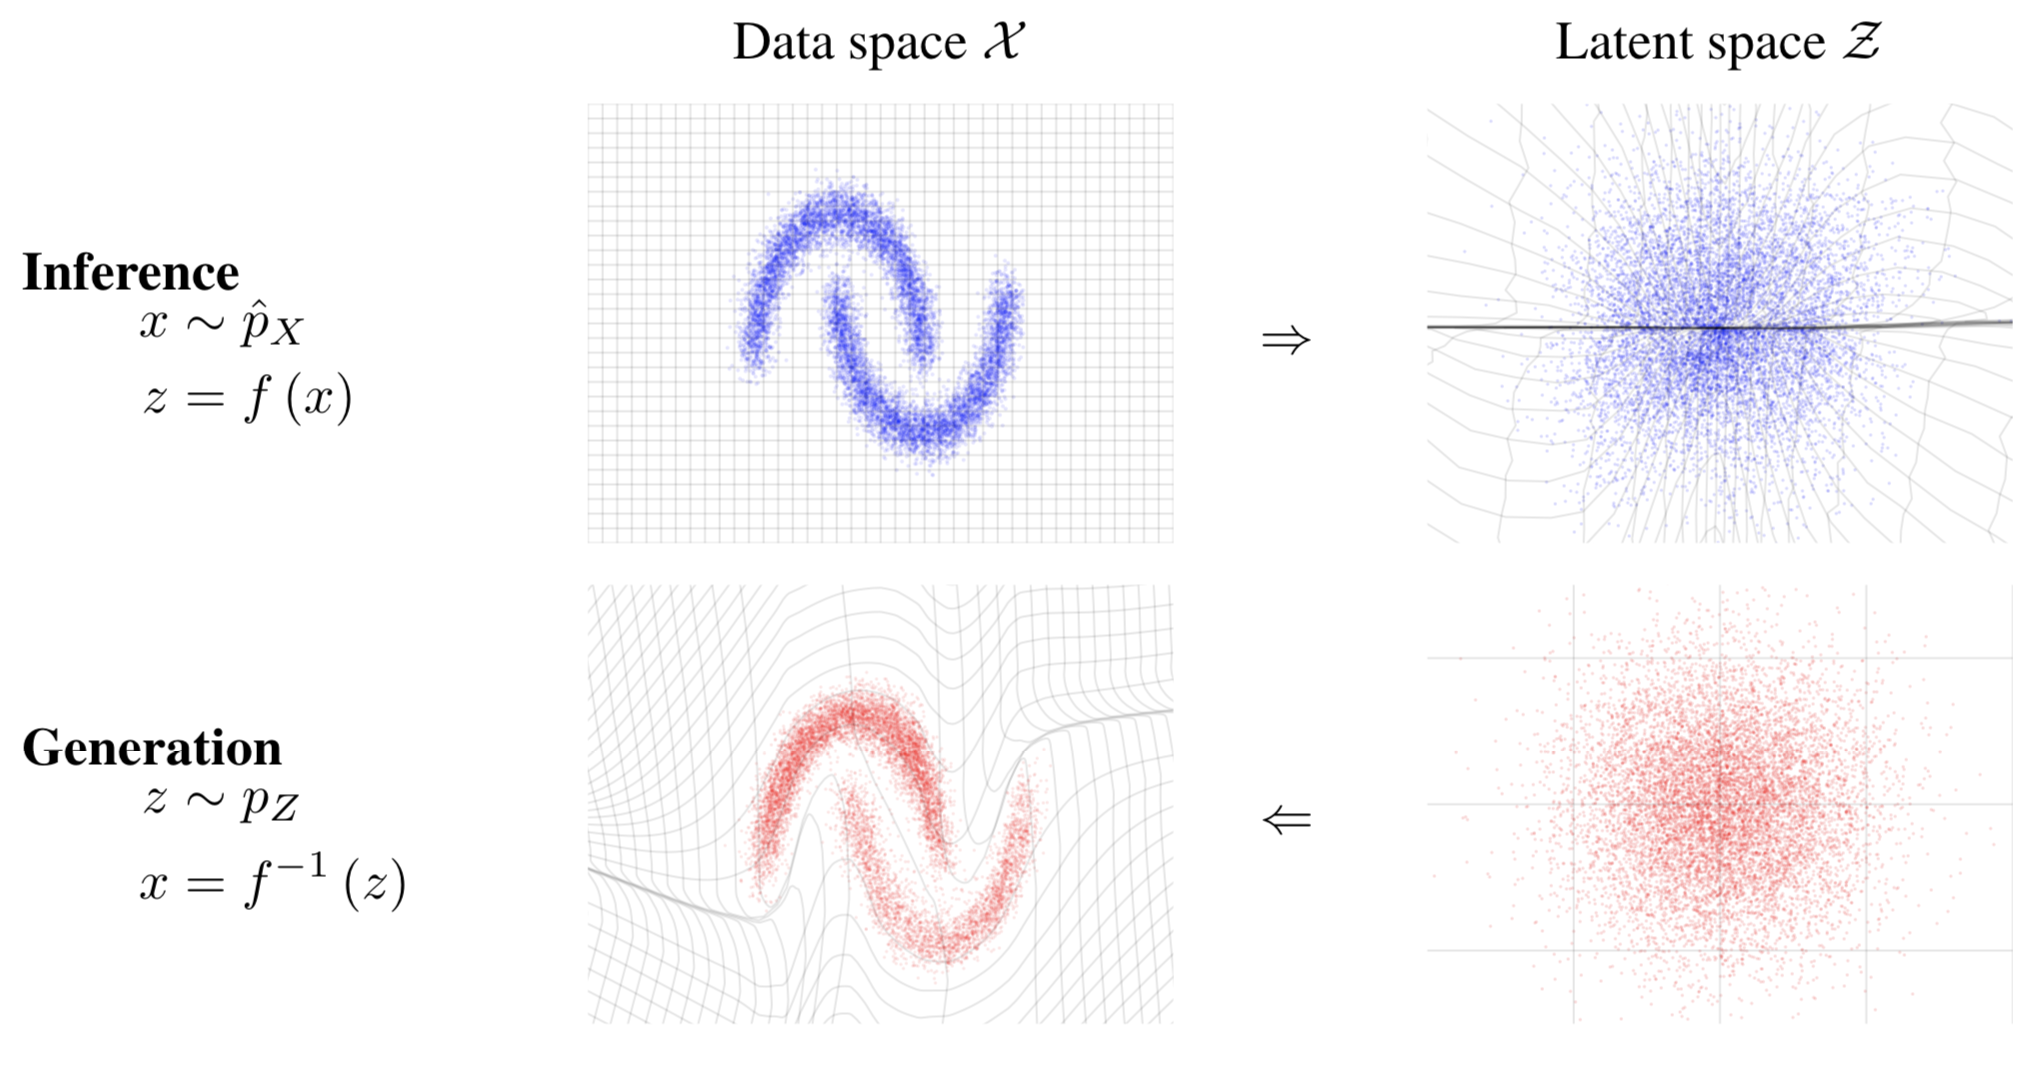
\includegraphics[width=0.5\linewidth]{chapters/petr_mokrov_s1/figs/flows_how2.png}
\end{figure}

При моделировании данных на многообразии классические нормализующие потоки обладают следующими недостатками: 
\begin{itemize}
    \item Распределение "размазанно" в окрестности целевого многообразия
    \item Вероятностная масса распределена в окрестности многообразия $\Rightarrow$ NF не моделирует истинную плотность
\end{itemize}
\begin{figure}[h]
    \centering
    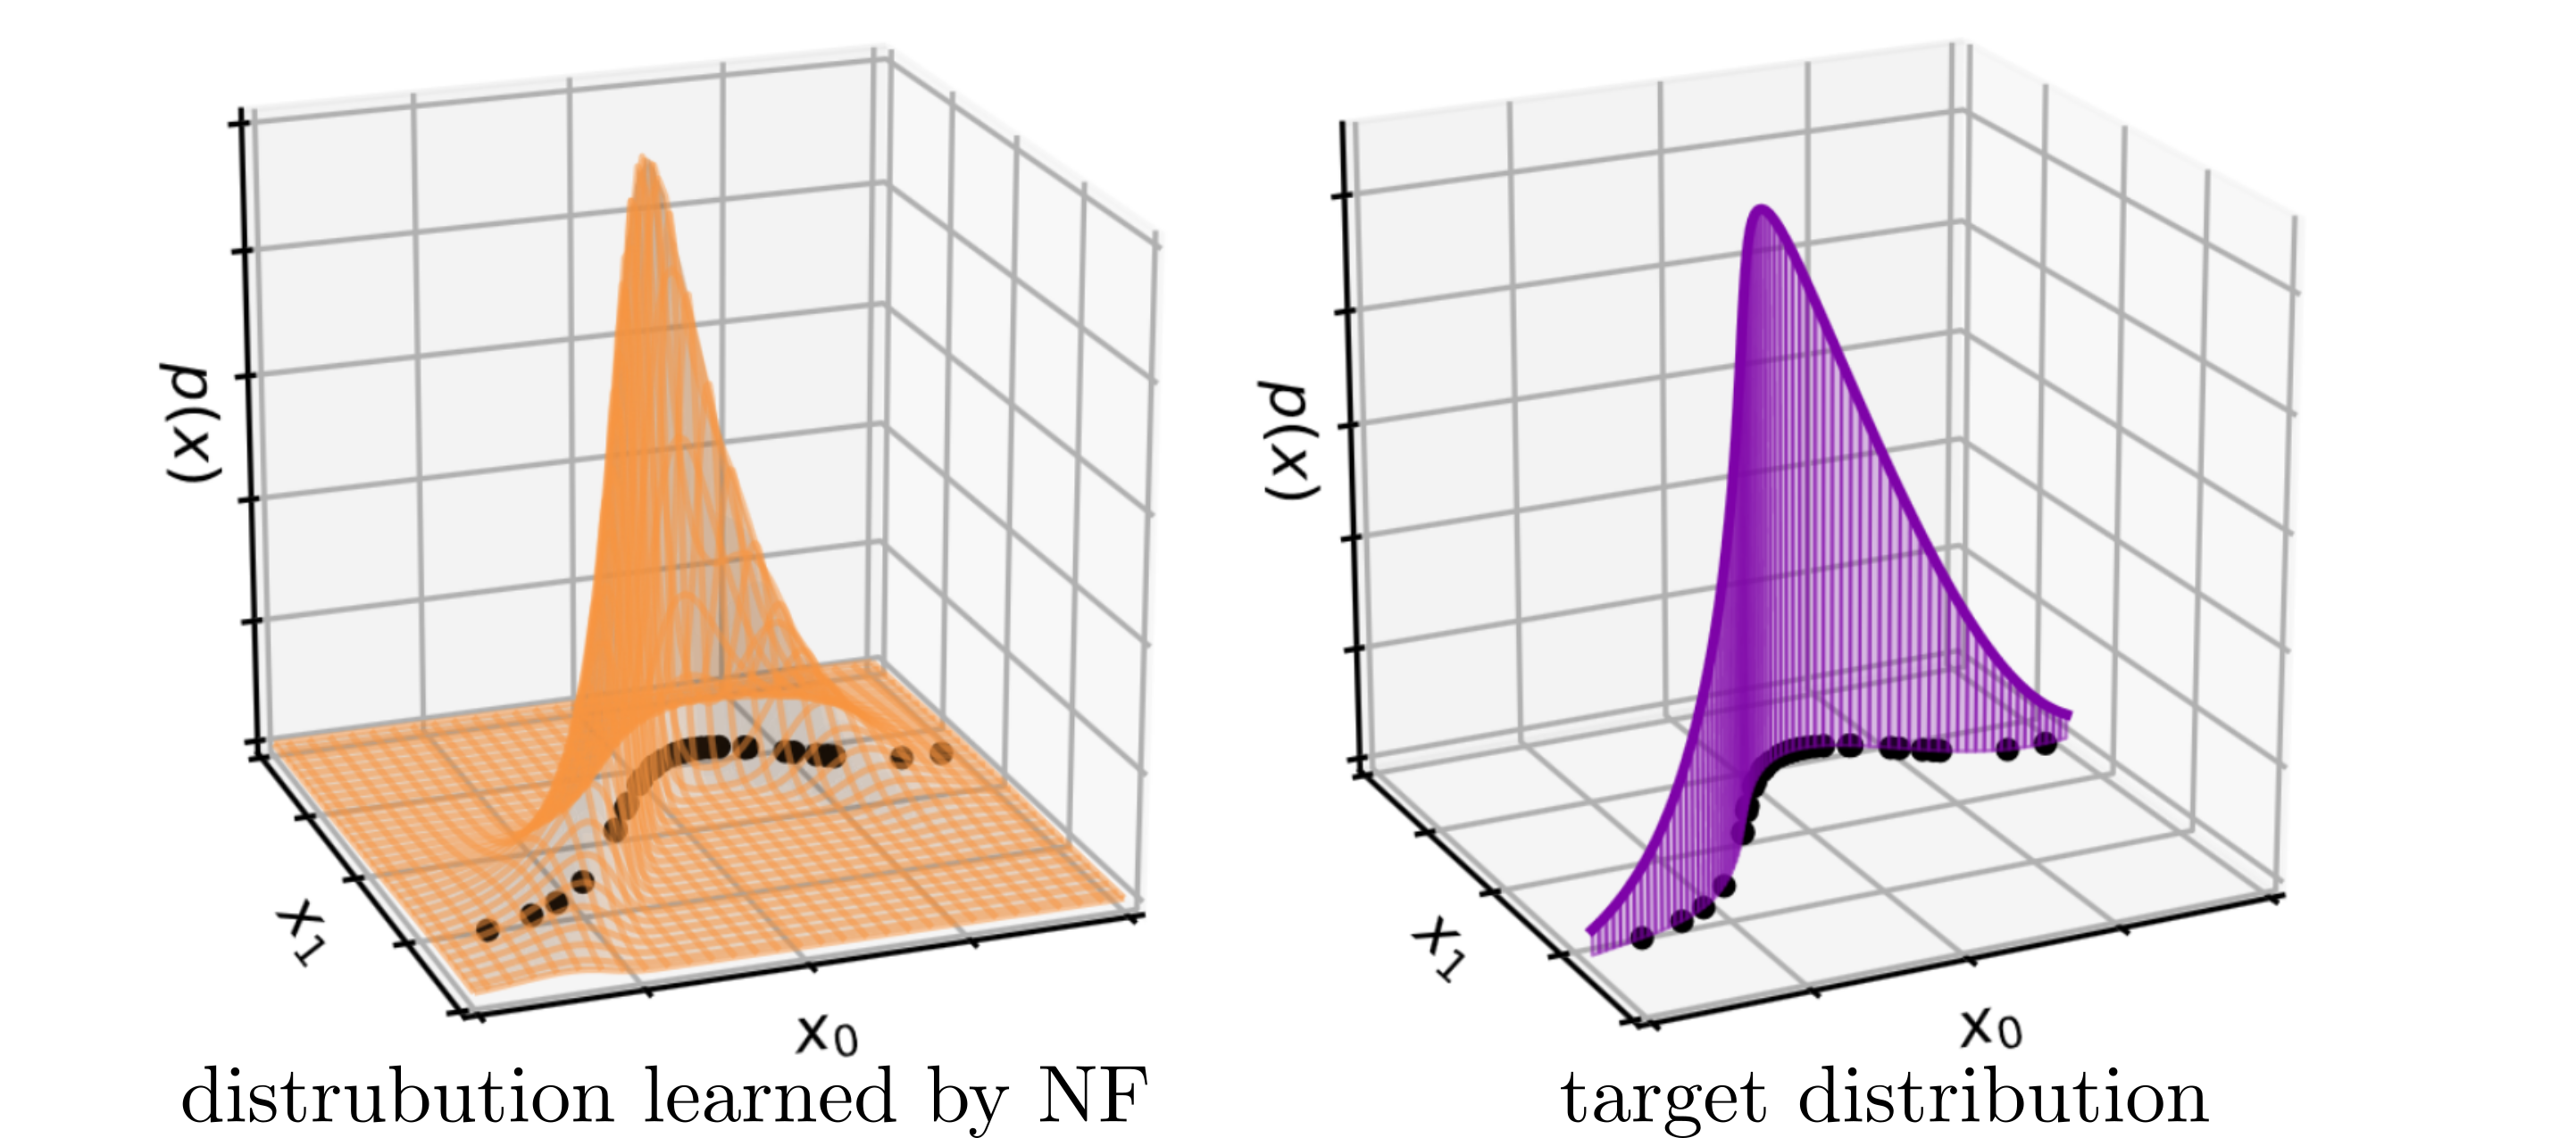
\includegraphics[width=0.6\linewidth]{chapters/petr_mokrov_s1/figs/nf_on_manifold_with_text.png}
\end{figure}

\newpage

\subsection{Notations}

Введём следующие обозначения: 

\begin{figure}[h]
    \centering
    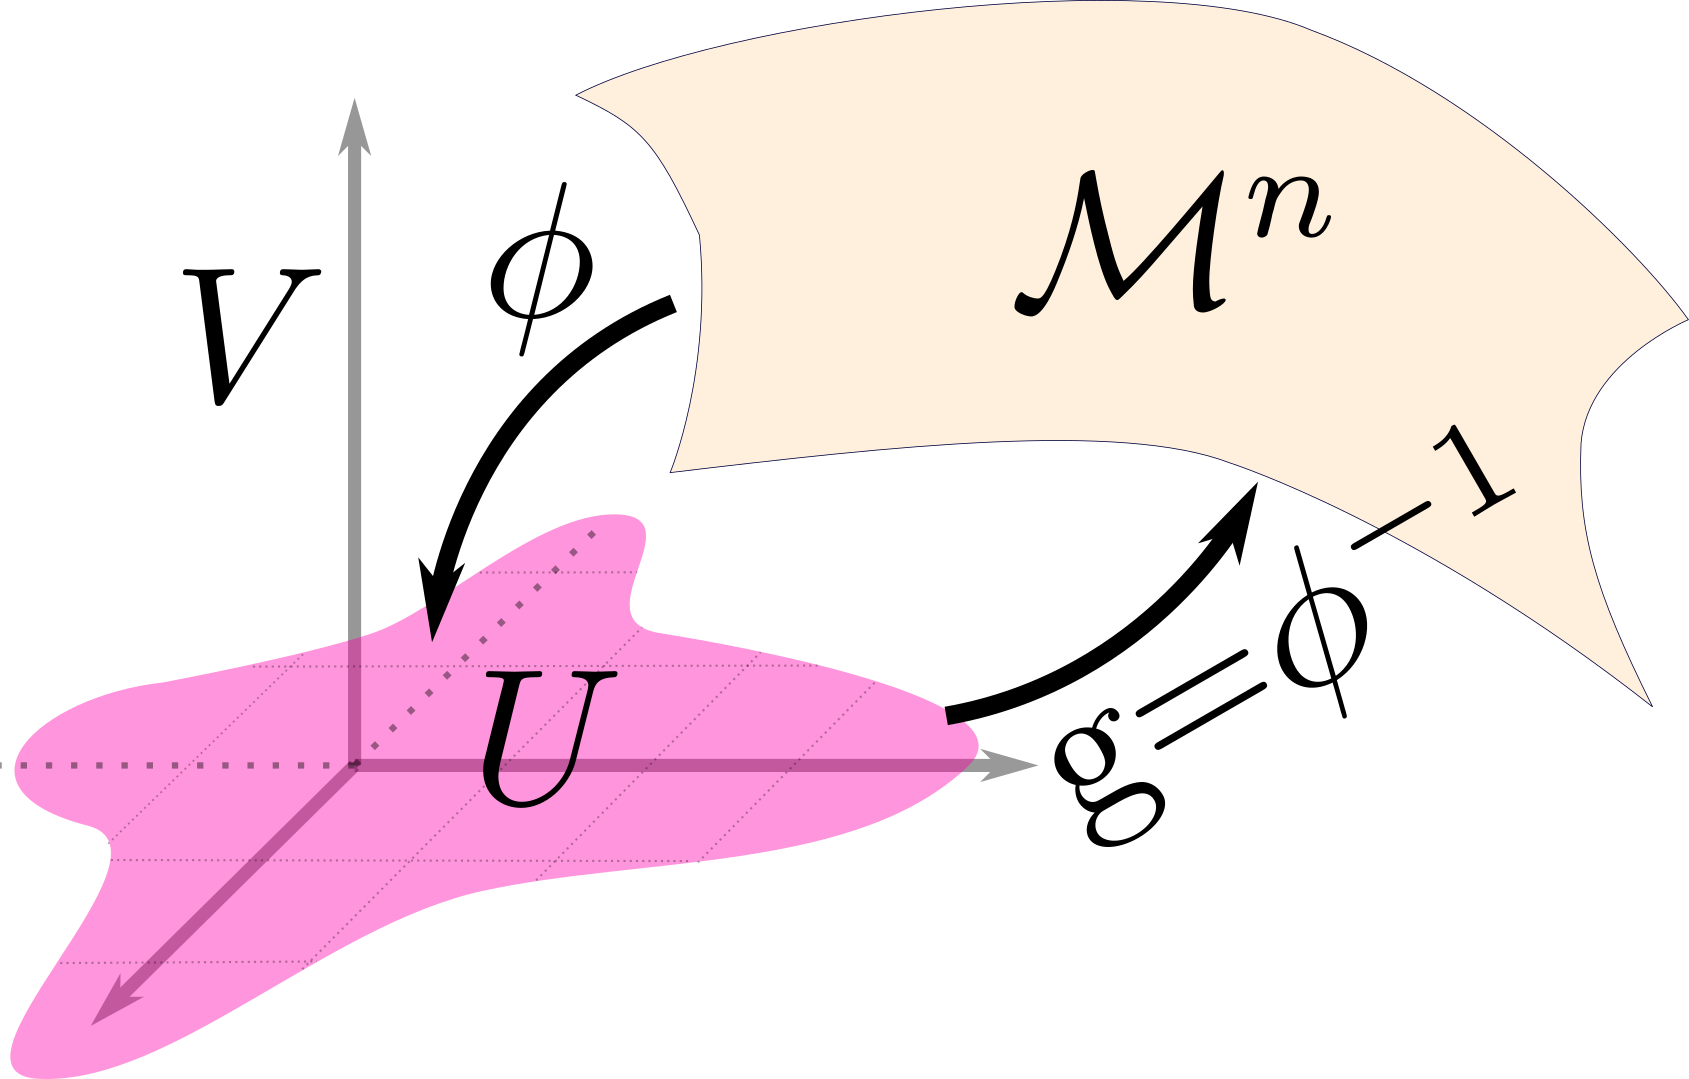
\includegraphics[width=0.4\linewidth]{chapters/petr_mokrov_s1/figs/notations4.png}
\end{figure}

\textbf{Manifold coordinates} В качестве $u \in U = \bbR^n$ мы будем обозначать вектора, которые отображаются в целевое многообразие $\cM^n$

\textbf{Off-the manifold coordinates} (остаточные координаты) В качестве $v \in V = \bbR^{N - n}$ мы будем обозначать оставшиеся координаты

\subsection{Flow on a manifold (FOM)}

В данном методе предполагается, что нам дано само многообразие и (обратная) карта: $g: U \rightarrow \cM^n$. Тогда верно следующее:

\begin{itemize}
    \item Из дифференциальной геометрии следует, что плотность на многообразии дана следующей формулой: 
    \begin{gather*}
        p_{\cM^n}(x) = p_{u}(g^{-1}(x)) \left|\det \left[J_g^T(g^{-1}(x)) J_g(g^{-1}(x))\right]\right|^{\frac{1}{2}} 
    \end{gather*}
    \item $J_g$ - якобиан карты $g$, матрица размера $n \times N$
    \item Плотность $p_u(u)$ в пространстве $U$ можно моделировать с помощью NF $$h : \tilde{U} (= U) \rightarrow U$$ рассматривая в качестве начальной плотности известную $p_{\tilde{u}}(\tilde{u})$
\end{itemize}

\begin{figure}[h]
    \centering
    \hspace*{-5mm}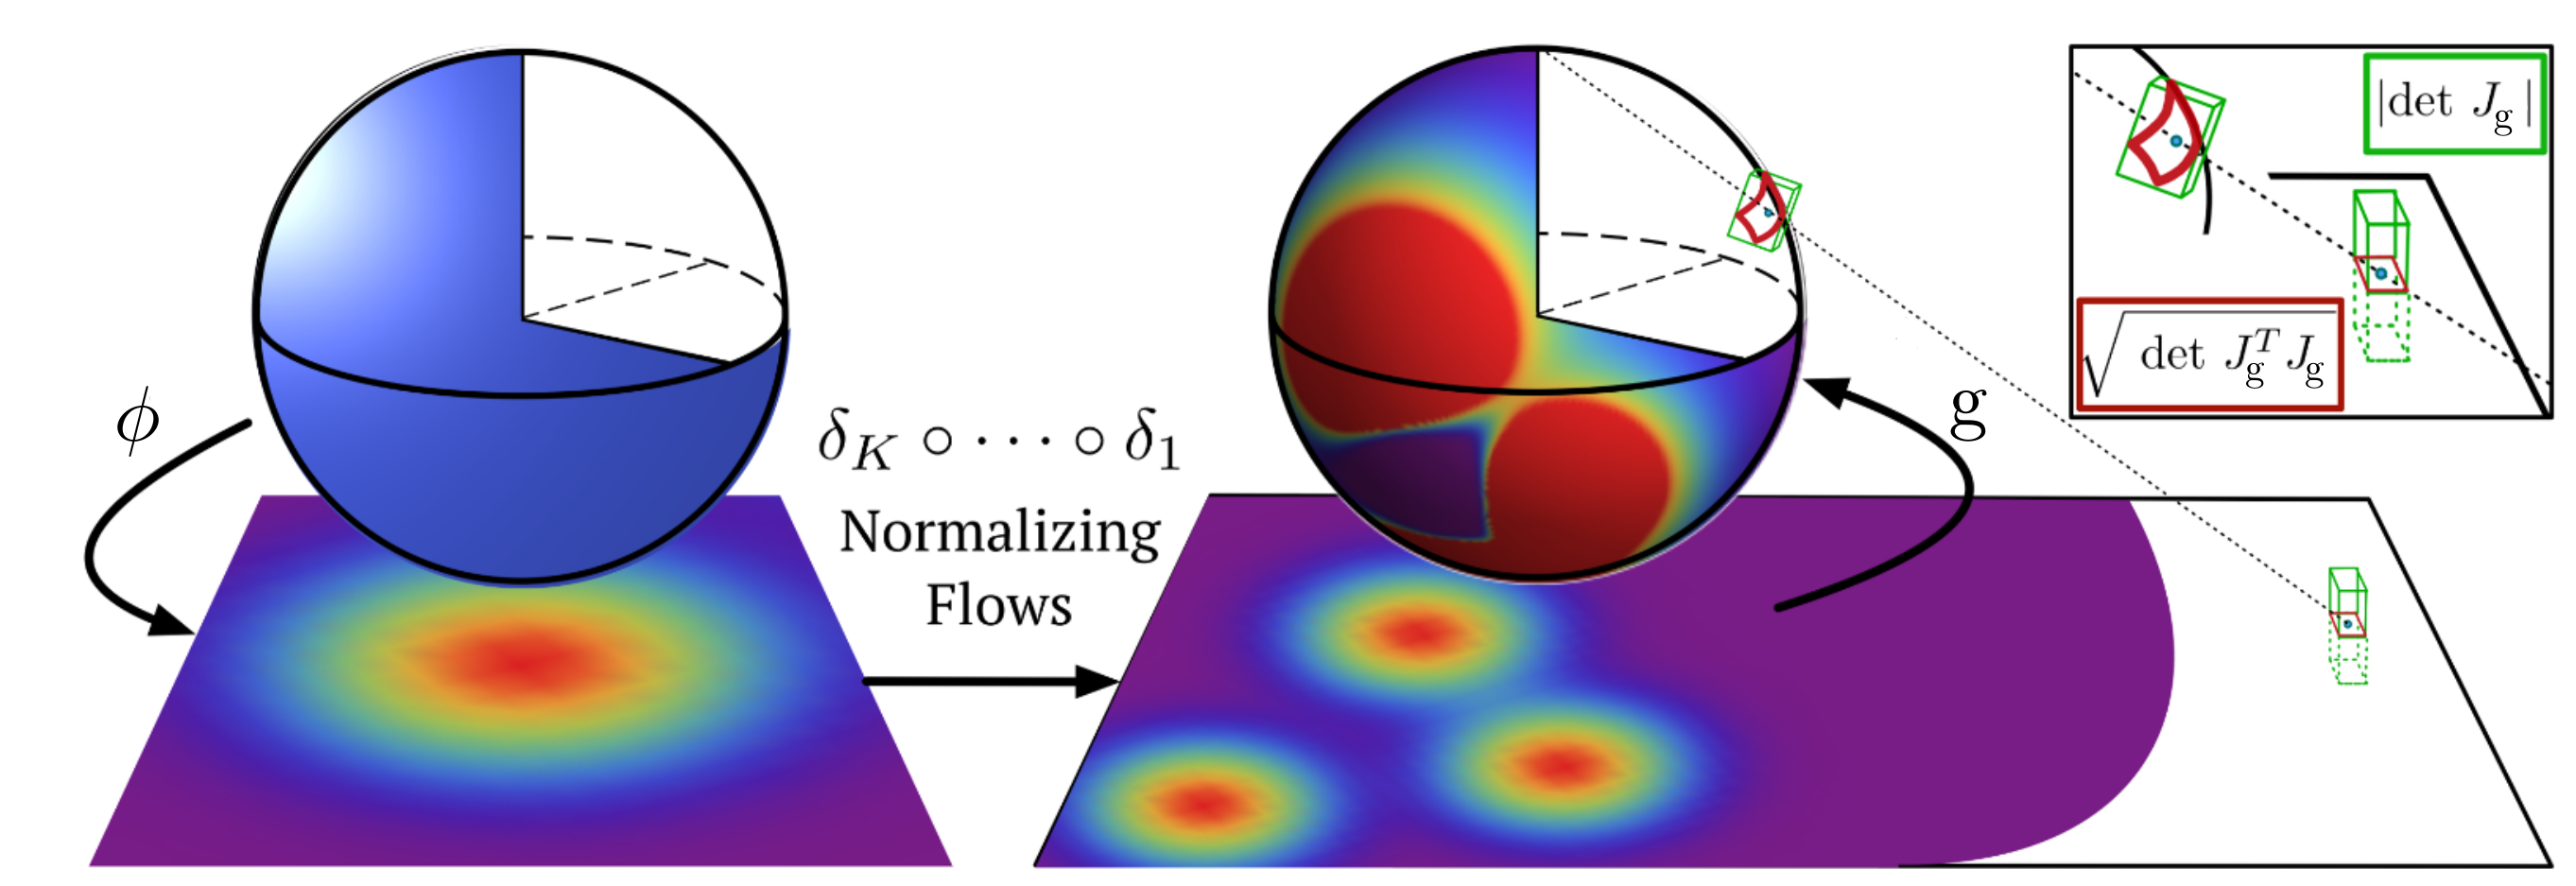
\includegraphics[width=0.7\linewidth]{chapters/petr_mokrov_s1/figs/fom_final.png}
\end{figure}

Достоинством данного подхода является возможность сведения задачи к классическим нормализующим потокам, важным недостатком явлется небоходимость знать карту целевого многообразия.

\newpage

\subsection{PIE: Pseudo-Invertible Encoder (V1)}

Одной из первых моделей, короая учит как плотность на многообразии, так и само многообразие, является PIE. 

\begin{figure}[h]
    \centering
    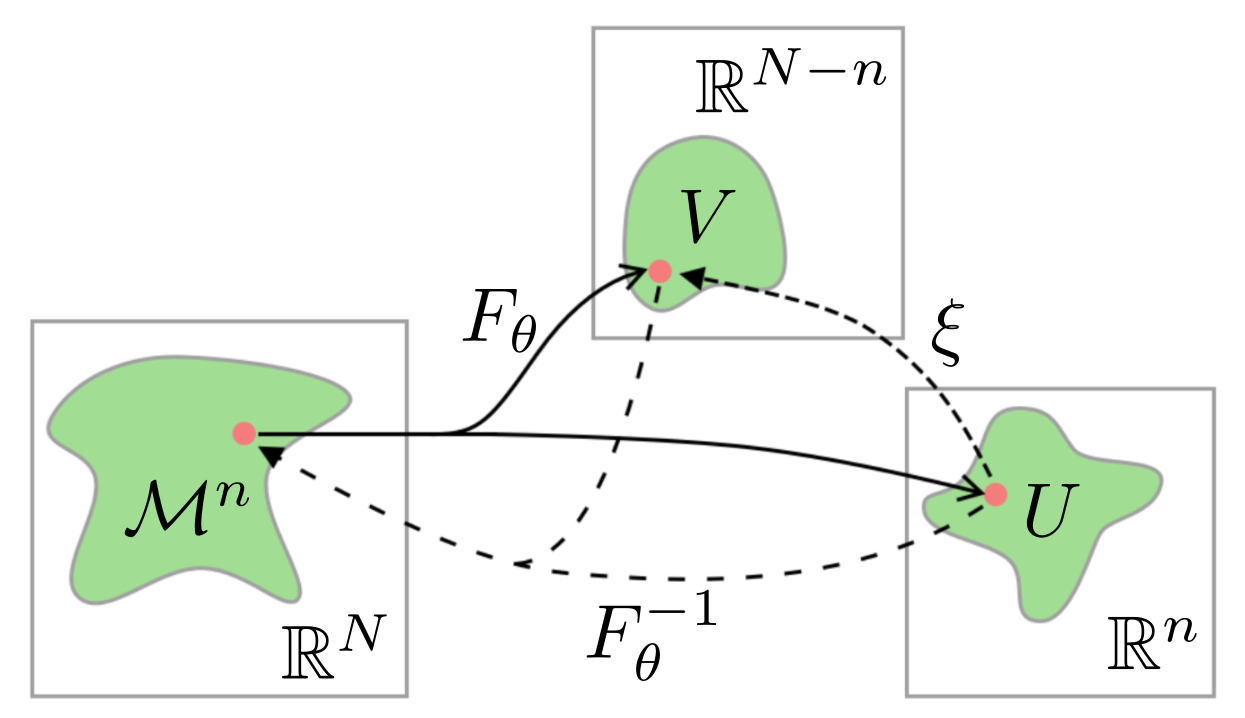
\includegraphics[width=0.5\linewidth]{chapters/petr_mokrov_s1/figs/pie_v1_final3.png}
\end{figure}

\begin{itemize}
    \item Модель по разному обрабатывает локальные координаты многообрзия $u \in U$ и остаточные координаты $v \in V$
    \item Вектор $v \in V$ генерируется из $u \in U$ с помощью фиксированной (или обучаемой) функции $\xi$
    \item Пара векторов $(u, v = \xi(u))$ преобразуется в точку на многообразии с помощью обучаемой модели $F_{\theta}^{-1}$ (поток $\bbR^N \rightarrow \bbR^N$)
\end{itemize}

На инференсе и при обучении модель работает следующим образом: 

\textbf{Genereative mode}
Для генерации семплируется $u \in U$, считается $v = \xi(u)$, преобразуется в целевую точку на многообразии $F_{\theta}^{-1}(u, \xi(u))$

\textbf{Log Likelihood}
Правдоподобие в точке на многообразии $x \in \cM^n$ оценивается так ($\epsilon_0$ - достаточно маленький): 
\vspace{-2mm}
\begin{gather*}
    \log p(x) = \log \det \left(J_{F_{\theta}}(x)\right) + \log p(u, v) \approx \\
    \approx \log \det \left(J_{F_{\theta}}(x)\right) + \log \cN(v | \xi(u), \epsilon_0 I) + \log p(z)
\end{gather*}

\green{Достоинства модели}: Модель учит целевое многообразие; обученная модель в generative mode семплирует из целевого многообразия

\red{Недостатки модели}: о построению нет критерия принадлежности точки многообразию; обучаемое распределение $p(x)$ не есть распределение на многообразии ($\log \det (J_{F_{\theta}}(x))$ - должно быть вырождено)

\newpage

\subsection{PIE: Pseudo-Invertible Encoder (V2)}

Была предложена модификация предыдущей модели, которая более явно разделяет обучение карты многообразия и плотности в пространстве координат: 

\begin{figure}[h]
    \centering
    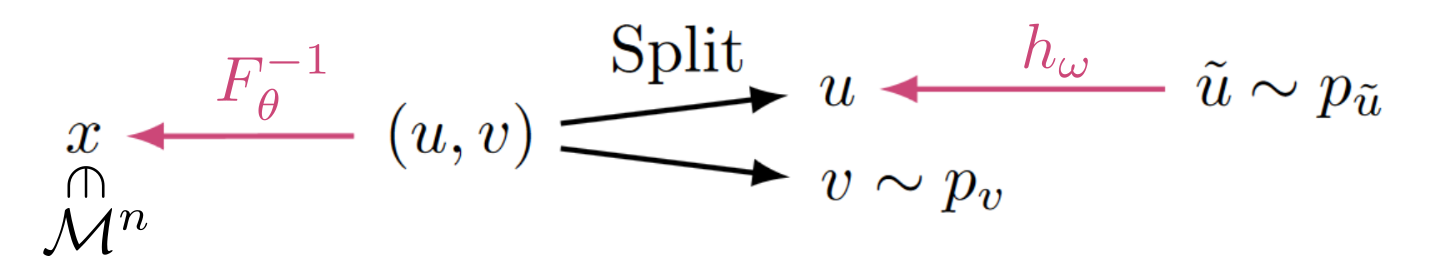
\includegraphics[width=0.6\linewidth]{chapters/petr_mokrov_s1/figs/pie_v2_final.png}
\end{figure}

Модель обладает следующими свойствами: 
\begin{itemize}
    \item Выбор функции $\xi$ не столь важен, берём $\xi = 0$
    \item Распределением $p_v$ служит $\cN(0, \epsilon_0 I)$
    \item Добавляем дополнительное отображение $h_{\omega}$ (поток $\bbR^n \rightarrow \bbR^n$), модифицирующее базовую плотность $p_{\tilde{u}}$ в пространстве координат
    \item \textbf{Note}: Интуитивно, мы бы хотели, чтобы $h_{\omega}$ учило правильную плотность в пространстве координат, а $F_{\theta}$ учило бы истинную карту многообразия $\cM^n$ 
\end{itemize}

Модель обладает теми-же недостатками, что и предыдущая модель. Для того, чтобы их решить, были предложены $\cM$ и $\cM_e$ потоки

\subsection{$\cM$-flow}

Предложенна модель удовлетворяет следующей схеме:

\begin{figure}[h]
    \centering
    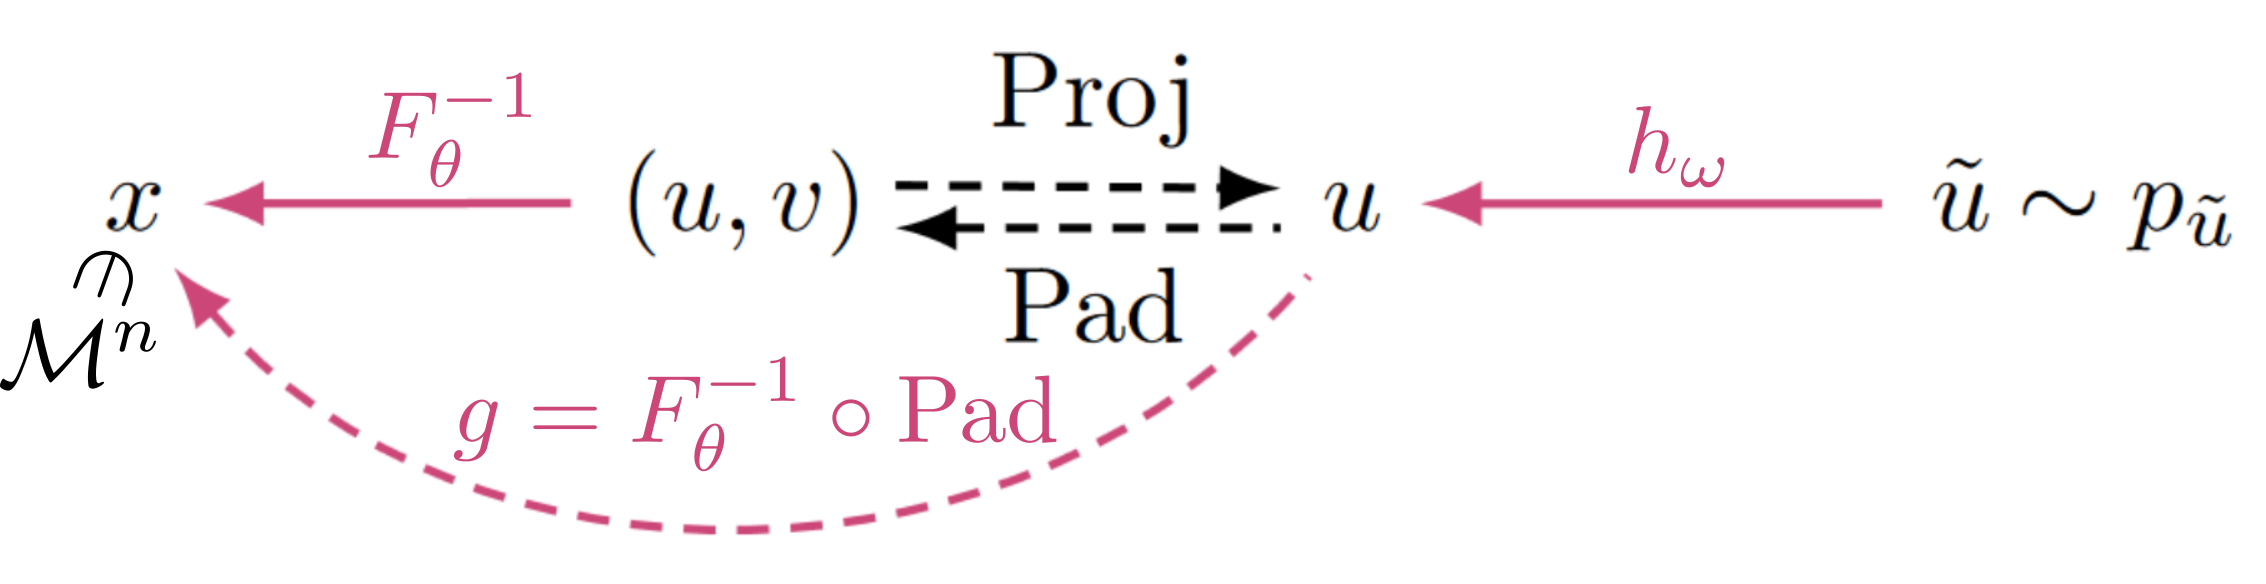
\includegraphics[width=0.6\linewidth]{chapters/petr_mokrov_s1/figs/mflow_final.png}
\end{figure}

Генерация и оценка правдоподобия делается следующим образом:

\textbf{Genereative mode}
Для генерации семплируется $u = h_{\omega}(\tilde{u}) \in U$, дополняется вектором $v = 0_{N - n}$ и преобразуется в целевую точку на многообразии $F_{\theta}^{-1}(u, 0_{N - n}))$

\textbf{Log Likelihood}
Правдоподобие в точке на многообразии $x \in \cM^n$:
\begin{gather*}
    \log p(x) = \log p_{\tilde{u}}(h_{\omega}^{-1}\circ g^{-1}(x)) - \log \det J_{h_{\omega}}(h_{\omega}^{-1}\circ g^{-1}(x)) - \\
    - 0.5 \log \det \left[ J_g^{T}(g^{-1}(x)) J_g(g^{-1}(x))\right]
    % \log \det \left(\frac{\partial F_{\theta}}{\partial x}\right) + \log p(u, v) \approx \\
    % \approx \log \det \left(\frac{\partial F_{\theta}}{\partial x}\right) + \log \cN(v | \xi(u), \epsilon_0 I) + \log p(z)
\end{gather*}

\subsubsection{Manifold chart learning}

Модель $\cM$ явным образом учит карту многообразия следующим образом: 
\begin{itemize}
    \item Поток $F_{\theta}$ в рамках всей модели учится представлять карту многобразия, для $x \in \cM^n$ минимизируемый лосс: 
    \vspace{-2mm}
    \begin{gather*}
        \cL_{\text{chart}} = \Vert x - g\left(\text{Proj}_{U}\left[F_{\theta}(x)\right]\right)\Vert
    \end{gather*}
    \item Имея $y \in \bbR^N$ карта $F_{\theta}$ определяет расстояние до многообразия: $\Vert y - g\left(\text{Proj}_{U}\left[F_{\theta}(y)\right]\right)\Vert$!
\end{itemize}

\begin{figure}[h]
    \centering
    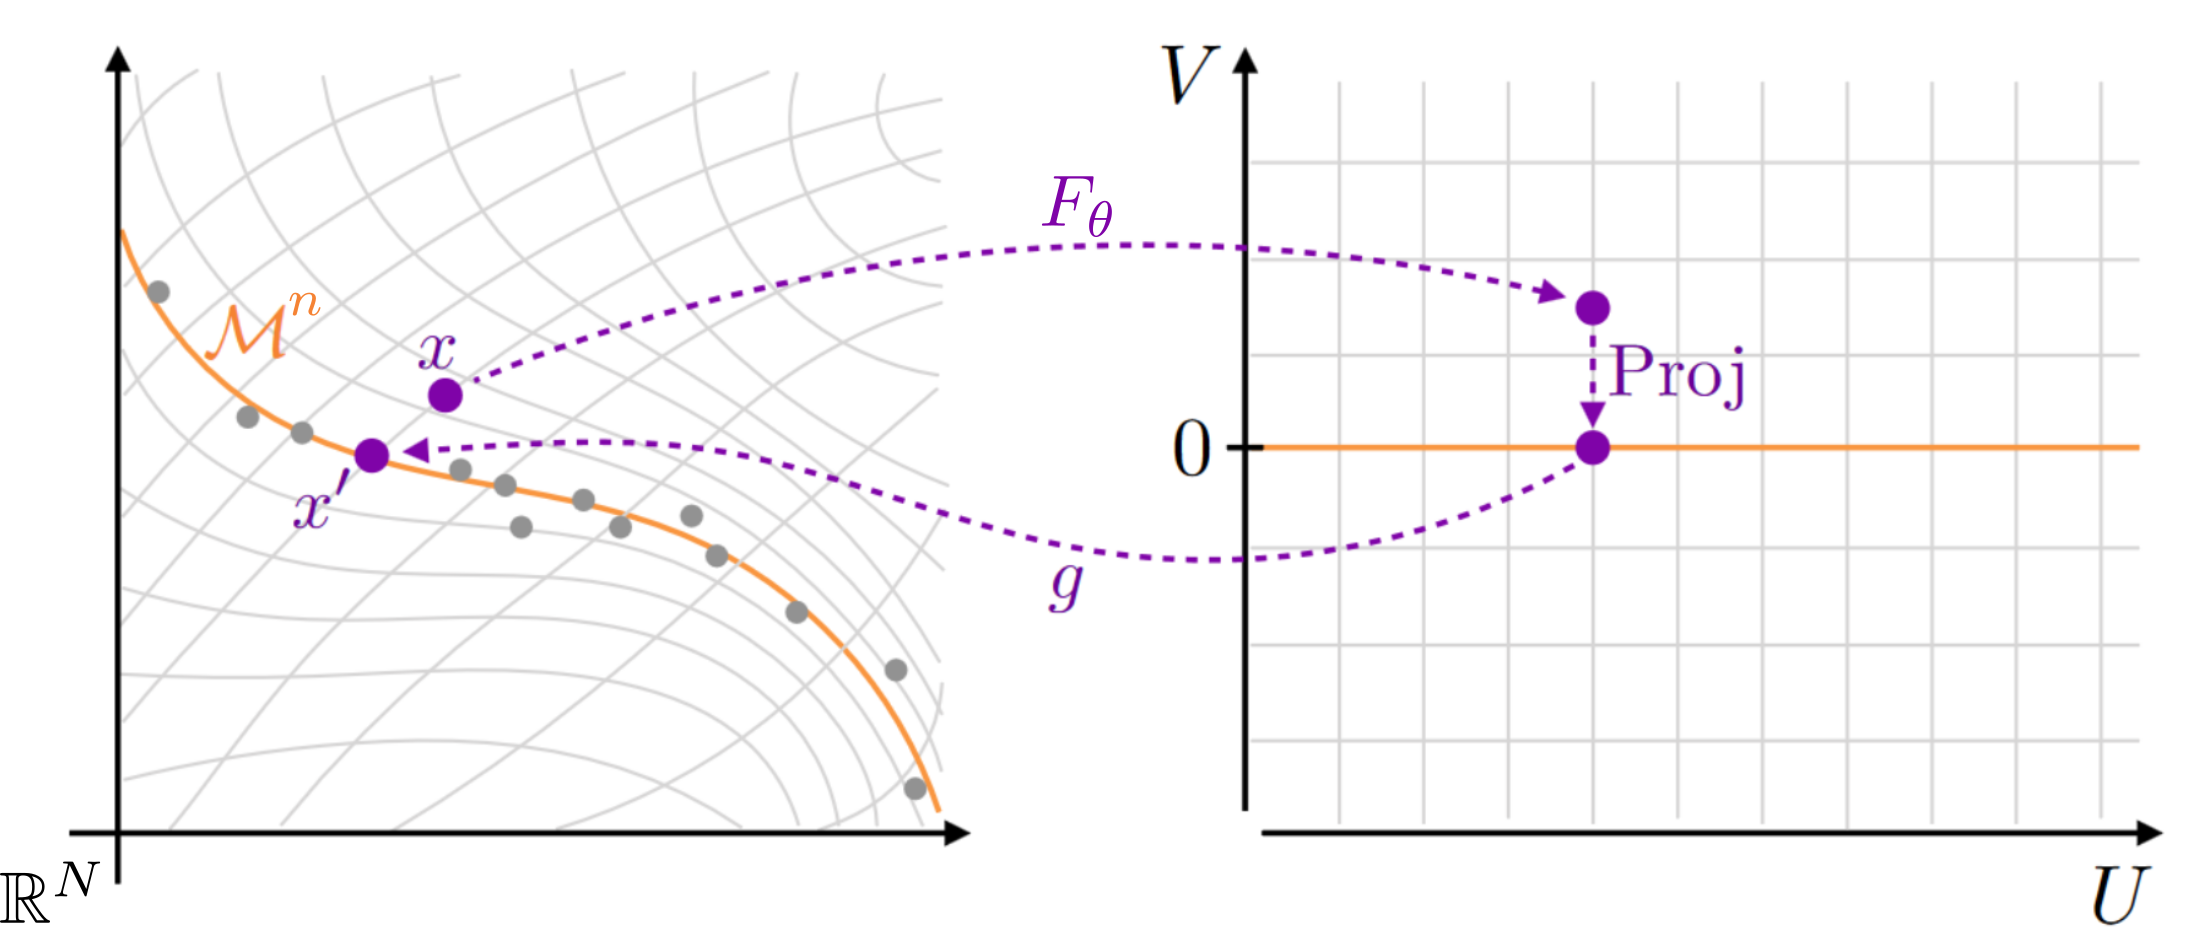
\includegraphics[width=0.6\linewidth]{chapters/petr_mokrov_s1/figs/mflow_manifold_final2.png}
\end{figure}

\subsubsection{Learning}

При обучении $cM$-потока чередуются два этапа: 
\begin{enumerate}
    \item Максимизация правдоподобия при фиксированной $F_{\theta}$
    \item Обучение карты $F_{\theta}$ при фиксированном распределении в пространстве координат $h_{\omega}\sharp p_{\tilde{u}}$ минимизируя лосс $\cL_{\text{chart}}$
\end{enumerate}

\subsection{$\cM_e$-flow}

Модифицированной версией $\cM$-потока является модель $\cM_e$-flow, представленная на схеме ниже: 

\begin{figure}[h]
    \centering
    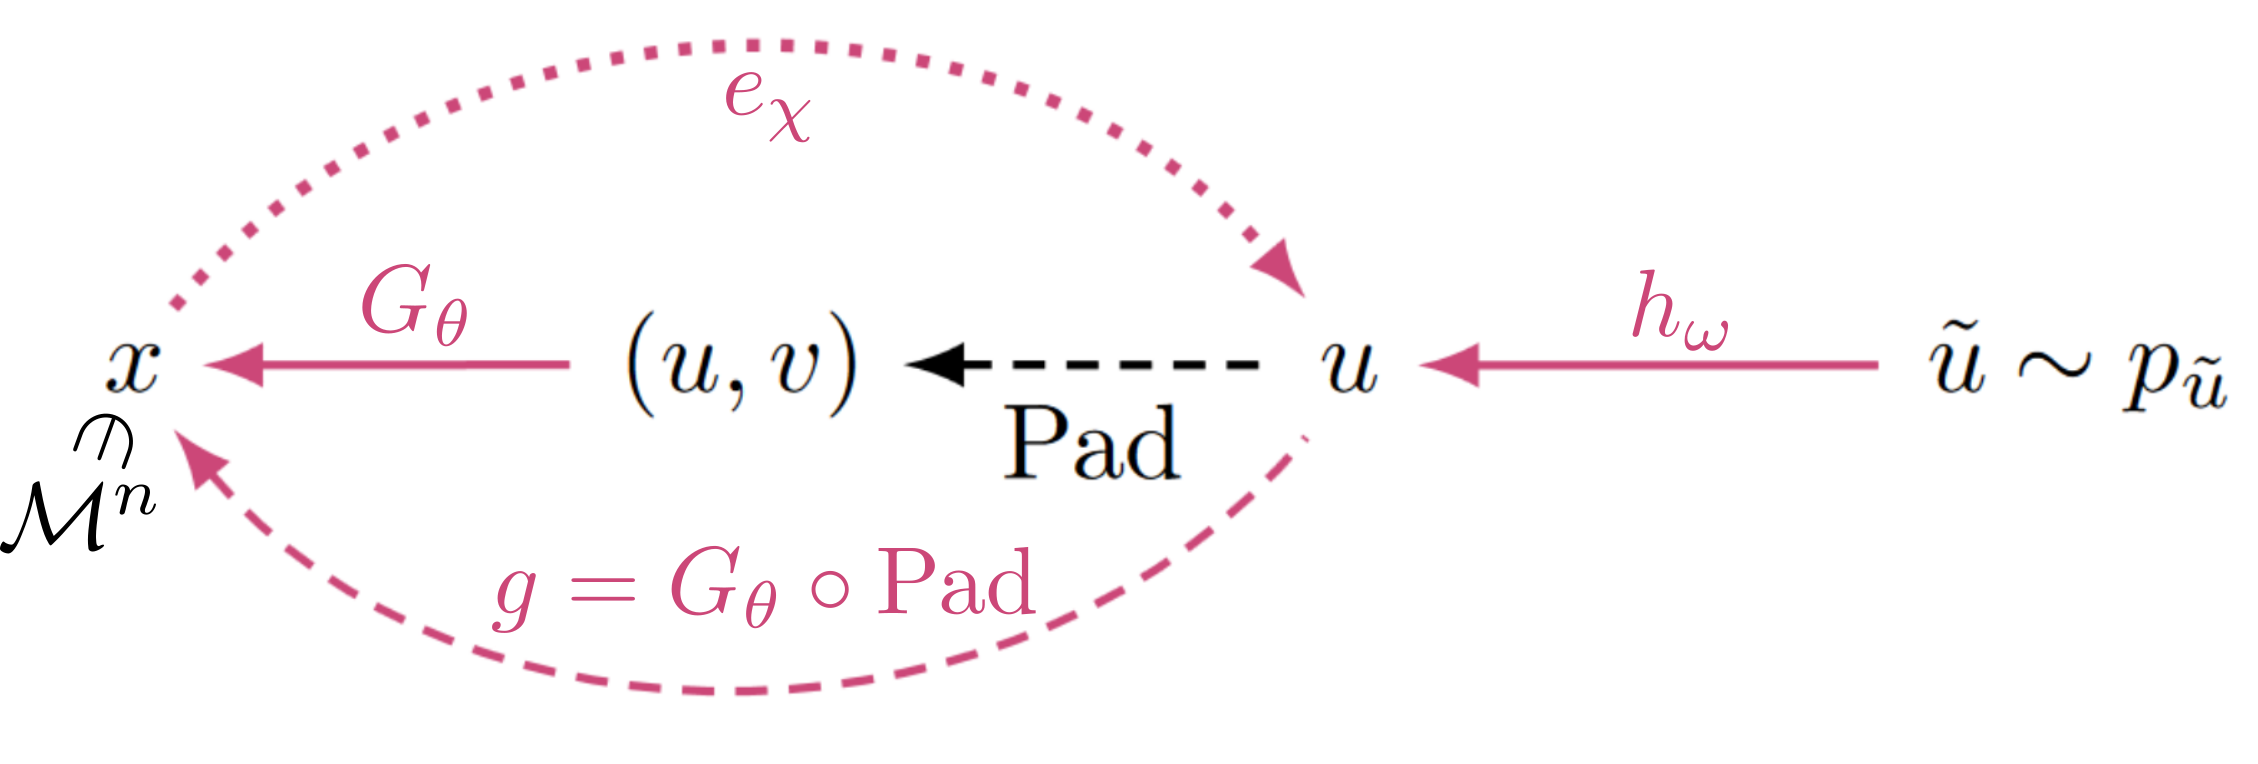
\includegraphics[width=0.6\linewidth]{chapters/petr_mokrov_s1/figs/mEflow_final.png}
\end{figure}

Особенности модели: 
\begin{itemize}
    \item Карта $g = G_{\theta} \circ \text{Pad}$ и (обратная) карта $e_{\chi}$ - разные модели
    \item $G_{\theta}$ и $e_{\chi}$ - не обязательно должны быть инвертируемы.
\end{itemize}

\newpage

\subsection{$\cM$ \& $\cM_{e}$-flows: Summary}

\textbf{\green{Достоинства модели}}
\begin{itemize}
    \item Модель явно учит карту многообразия $F_{\theta}$
    \item Естественным образом формулируется расстояние и проекция точки $y \in \bbR^N$ на многообразие $\cM^n$
    \item Легко оценивать отношение плотностей в байесовском инференсе (позднее!)
\end{itemize}
\textbf{\red{Недостатки модели}}
\begin{itemize}
    \item Вычисление плотности - \textbf{дорогое}, из-за необходимости вычисления якобиана карты: $\det \left[ J_g^{T}(g^{-1}(x)) J_g(g^{-1}(x))\right]^{\frac{1}{2}}$
    \item При раздельном обучении карты $F_{\theta}$ и плотности в пространсте координат $h_{\omega}$ карта может делать сжатия/растяжения, усложняющие обучение модели плотности.
\end{itemize}

В дальнейших секциях мы рассмотрим различные модельные задачи, а также приложения изученных моделей

\subsection{Test case: Gaussian on a Circle}

В даном эксперименте в качестве многообразия рассматривается круг, распределение на многообразии дано распределением на полярных угловых координатах $\theta \sim \cN(\pi/2, \pi/4)$

\begin{figure}[h]
    \centering
    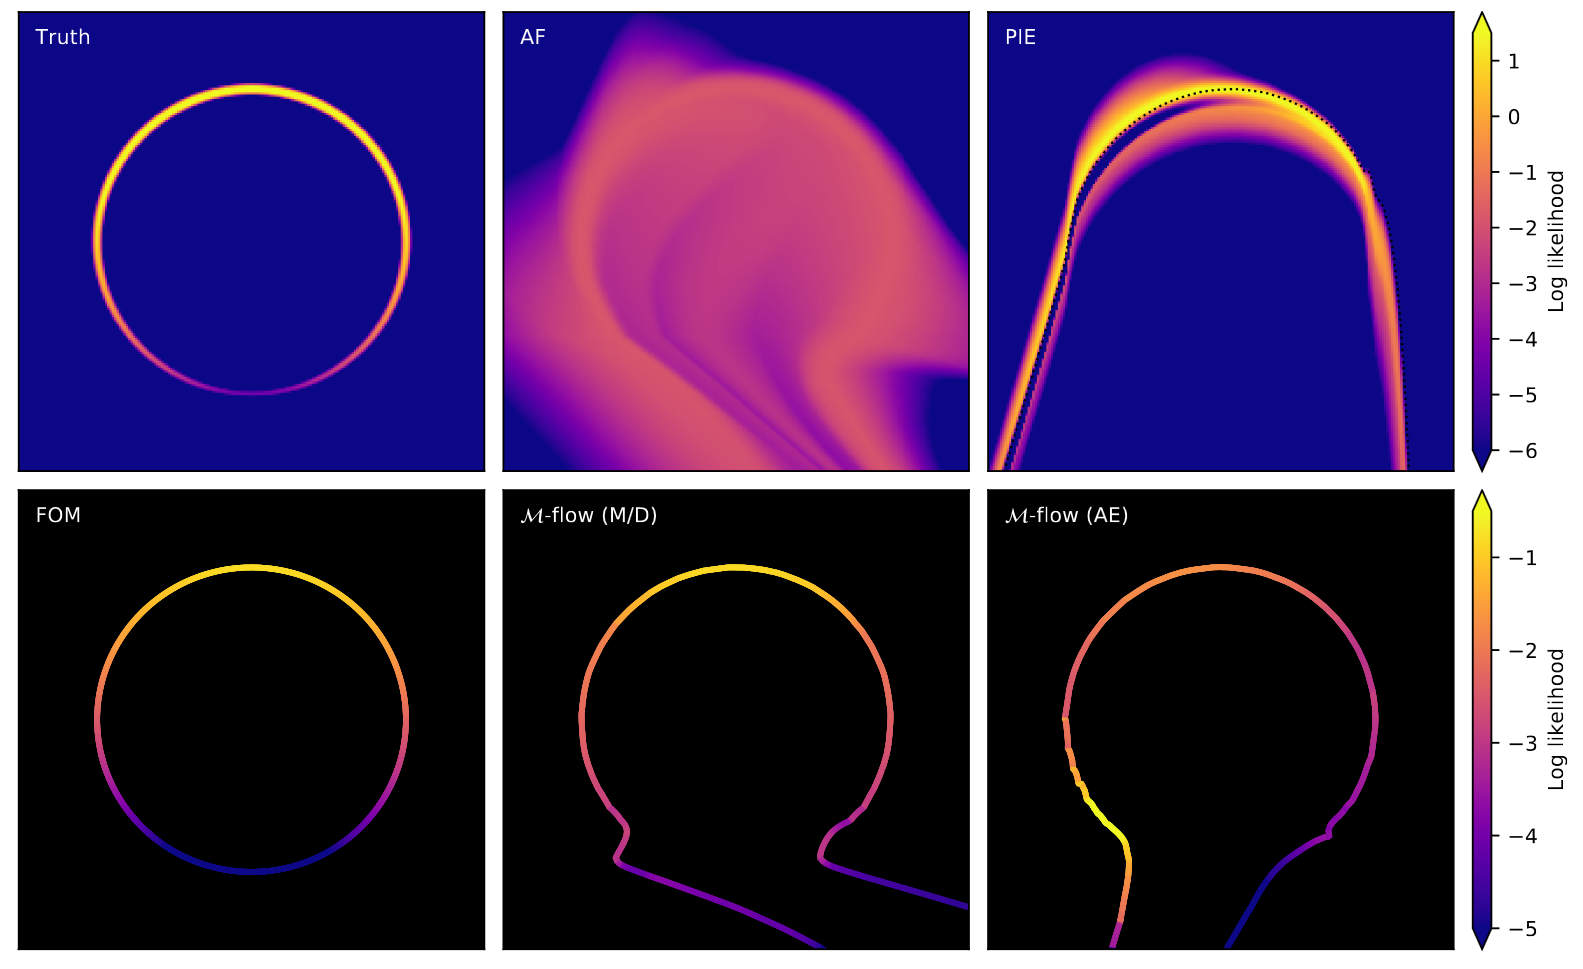
\includegraphics[width=0.7\linewidth]{chapters/petr_mokrov_s1/figs/gauss_in_circ.png}
\end{figure}

AF - классический нормализующий поток; Модель $\cM$-flow (AE) в отличие от $\cM$-flow (M/D) обучалась только правильно отражать координаты в многообразие.

\newpage

\subsection{Test case: Lorenz attractor}

Рассматривается Аттрактор Лоренца - Геометрическое Место траекторий дифференциального уравнения: 
\begin{gather*}
\begin{cases}
dx_0/dt = \sigma(x_1 - x_0) \\
dx_1/dt = x_0(\rho - x_2) - x_1\\
dx_2/dt = x_0 x_1 - \beta x_2
\end{cases}\\
\sigma=10, \beta = 8/3, \rho=28
\end{gather*}
% $\sigma=10, \beta = 8/3, \rho=28$

Аттрактор Лоренца образует многообразие размерности $\approx 2$. Для моделирования используются $\cM$-flows, обучаются на точках, равномерно распределённых на траекториях.

\begin{figure}[h]
    \centering
    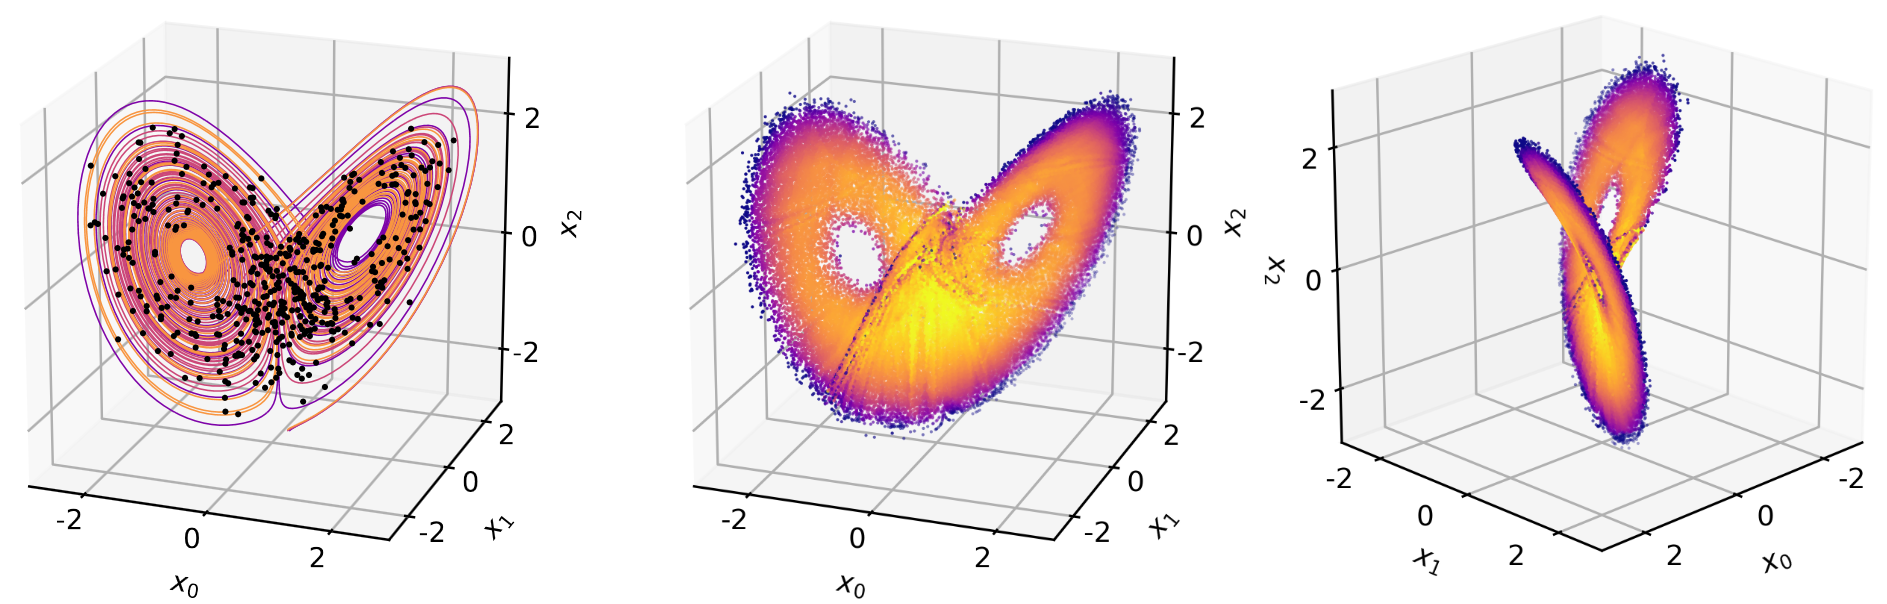
\includegraphics[width=0.7\linewidth]{chapters/petr_mokrov_s1/figs/lorenz_attractor.png}
\end{figure}

На левом рисунке изображены истинные траектории дифференциального уравнения с просемплированными точками. На правых двух рисунках изображено выученное многообразие.

\subsection{Likelihood-free simulation-based inference}

Рассмотрим задачу likelihood-free simulation-based inference. Данная задача формулируется следующим образом: 
\begin{itemize}
    \item Дан симулятор $p_{\text{model}}(x | \zeta)$, описывающая некоторую физическую реальность обусловленную на параметры модели/константы природы (плотность не дана!)
    \item Требуетcя вычислить апостериорную плотность (Bayesian inference):
    \vspace{-2mm}
    \begin{gather*}
        p(\zeta | X) = \frac{p(X | \zeta) p(\zeta)}{\int_{Z} d \zeta' p(X | \zeta') p(\zeta')}
    \end{gather*}
\end{itemize}

\newpage

На рисунке ниже изображены примеры симуляторов: слева показана модель, семплирующая картинку из MNIST по параметру - цифре. Справа схематически показана модель, расчитывающая какие-либо физические экспериментальные величины (спектры поглощения/излучения частиц, например) чёрной дырой по массе и угловой скорости чёрной дыры 

\begin{figure}[h]
    \centering
    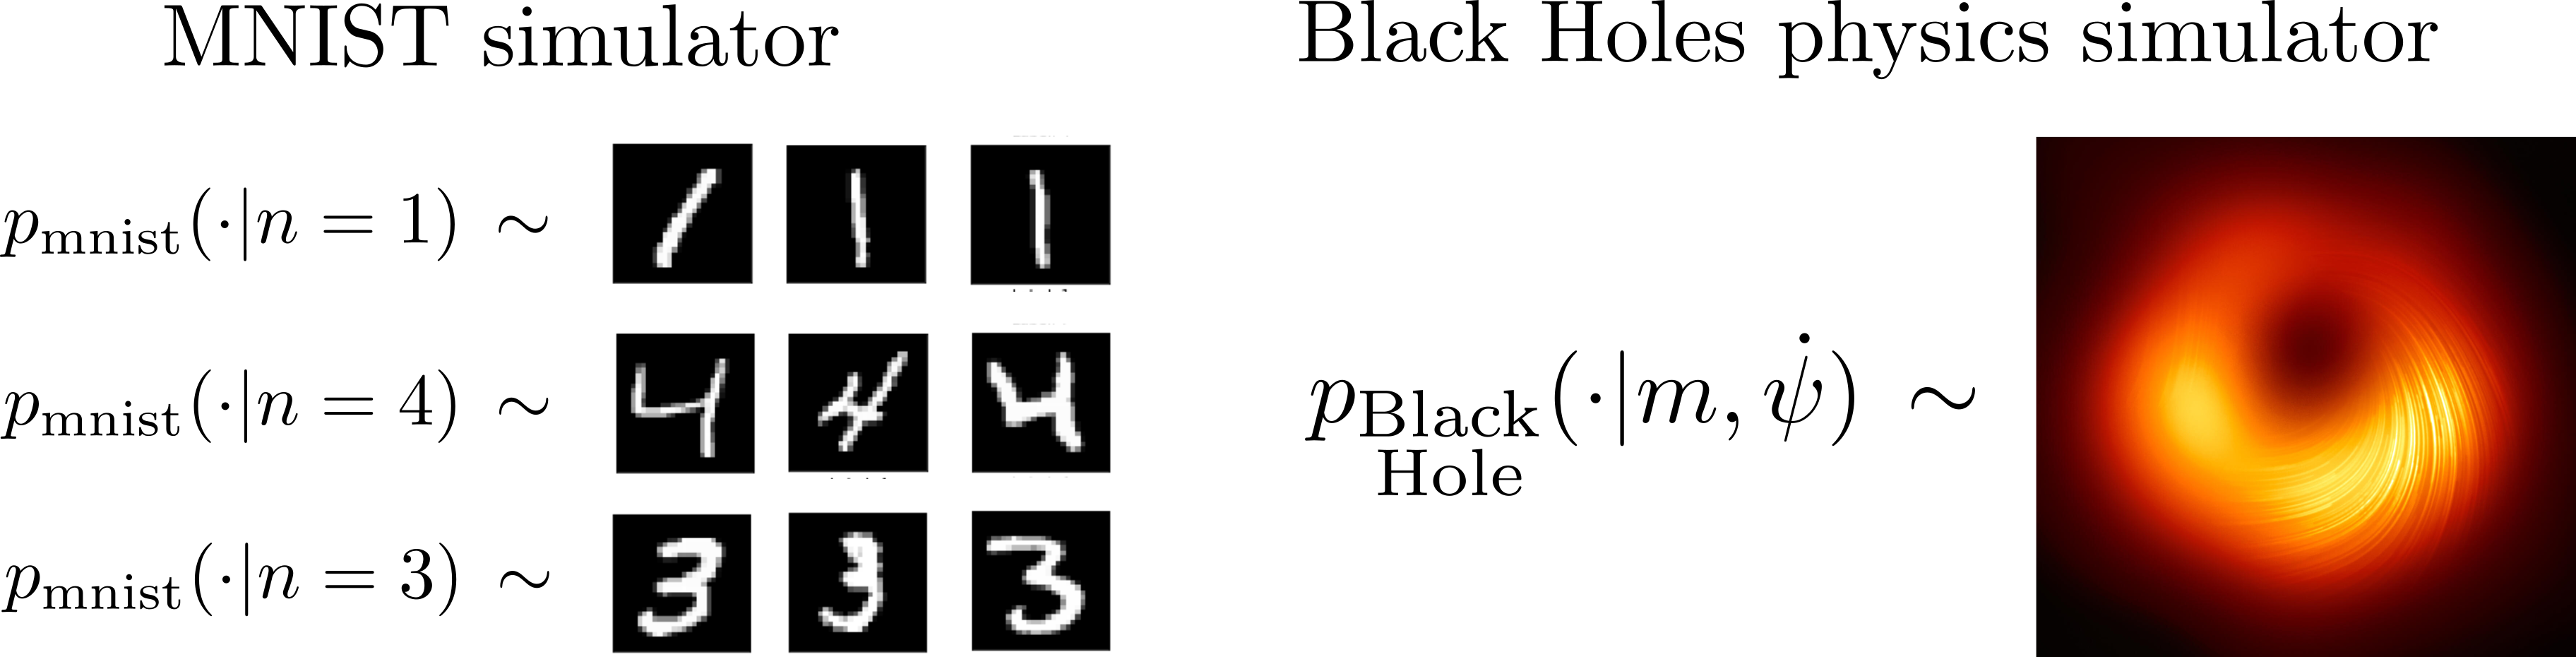
\includegraphics[width=0.7\linewidth]{chapters/petr_mokrov_s1/figs/simulators_demo.png}
\end{figure}

\subsubsection{$\cM$-flows for simulation-based inference}

Напомним схему $\cM$-потока: 
\begin{figure}[h]
    \centering
    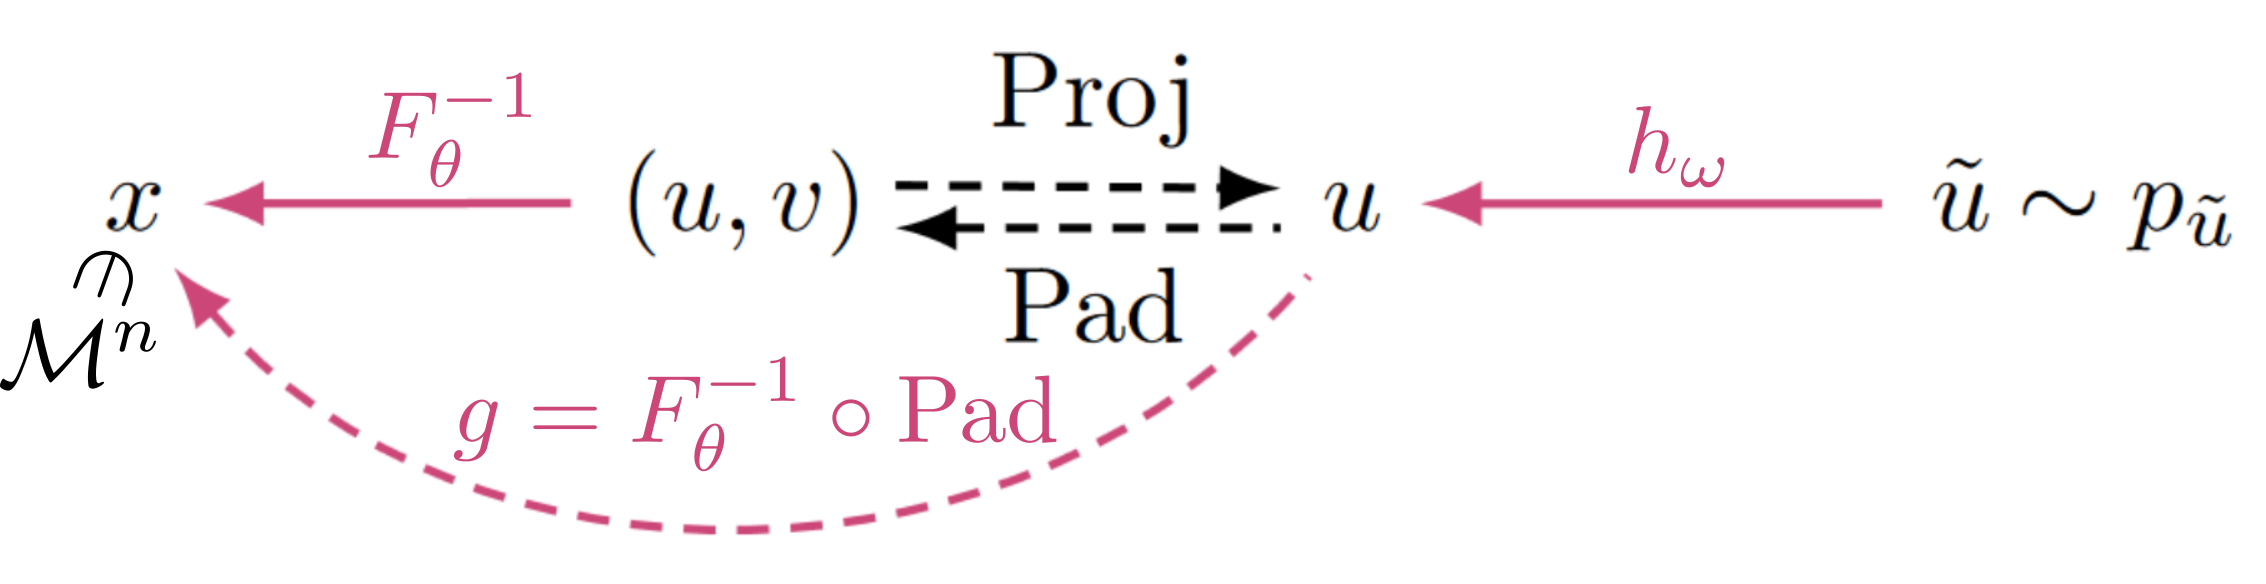
\includegraphics[width=0.6\linewidth]{chapters/petr_mokrov_s1/figs/mflow_final.png}
\end{figure}

Пусть многообразие $\cM^n$ \textbf{не зависит} от параметра $\zeta$. Тогда плотность на многообразии имеет следующий вид:
\begin{gather*}
    p(x| \zeta) = p_{\tilde{u}}(h_{\omega}^{-1}\left\{g^{-1}(x)| \zeta\right\}) \cdot \det J_{h_{\omega}}\left[h_{\omega}^{-1}\left\{g^{-1}(x)| \zeta\right\}\right]^{-1} \cdot \\ \cdot \det \left[ J_g^{T}(g^{-1}(x)) J_g(g^{-1}(x))\right]^{\frac{1}{2}}
\end{gather*}
При этом отношение плотностей при разных значениях параметра $\zeta$ не зависит от якобиана карты! ($\Rightarrow$ нам его не нужно вычислять):
\begin{gather*}
        \frac{p(x|\zeta_1)}{p(x|\zeta_2)} = \frac{p_{\tilde{u}}(h_{\omega}^{-1}\left\{g^{-1}(x)| \zeta_1\right\}) \cdot \det J_{h_{\omega}}\left[h_{\omega}^{-1}\left\{g^{-1}(x)| \zeta_1\right\}\right]^{-1}}{p_{\tilde{u}}(h_{\omega}^{-1}\left\{g^{-1}(x)| \zeta_2\right\}) \cdot \det J_{h_{\omega}}\left[h_{\omega}^{-1}\left\{g^{-1}(x)| \zeta_2\right\}\right]^{-1}}
\end{gather*}

\newpage

Это свойство можно использовать в алогоритме Метрополиса-Гастингса для MCMC семплирования из апостериорной плотности $p(\zeta|X)$: 
\begin{figure}[h]
    \centering
    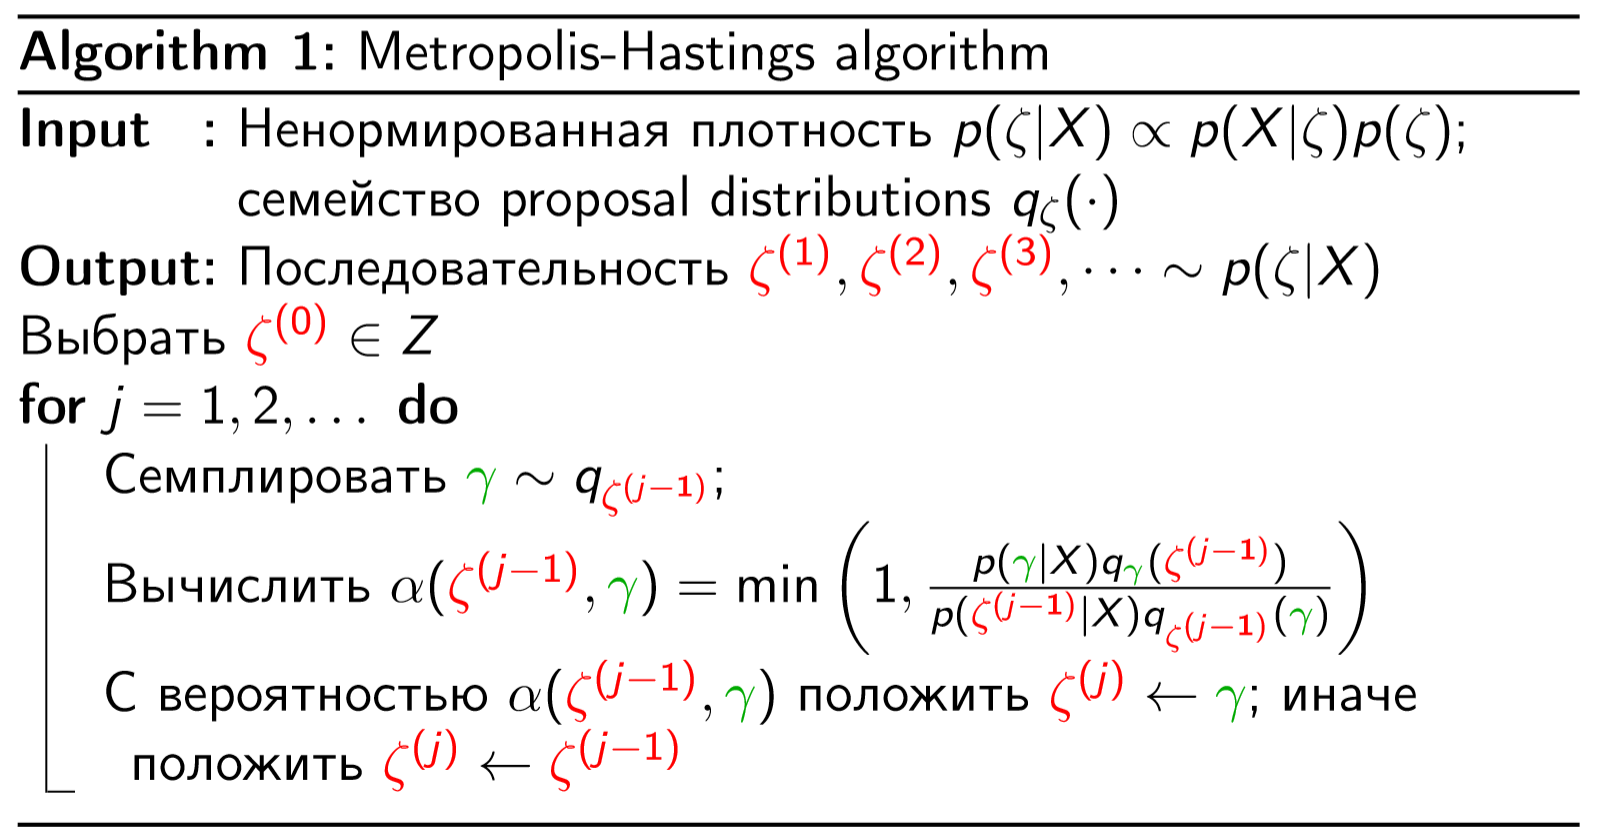
\includegraphics[width=0.8\linewidth]{chapters/petr_mokrov_s1/figs/metr_hast.png}
\end{figure}

\subsection{Application: Particle Physics}

Рассмотрим применение изученных нами потоков на многообразиях в контексте Likelihood-free simulation-based inference для решения задачи из физики частиц

Исследуется симулятор столкновения протонов в LHC. Параметрами модели выступают коэффициенты эффективной теории поля $\zeta \in \bbR^3$, семплируется набор статистик $x \in \bbR^{40}$. Из физики известно, что данные лежат на $14$-D многообразии.

Результаты работы моделей представлены на таблице ниже: 

\begin{figure}[h]
    \centering
    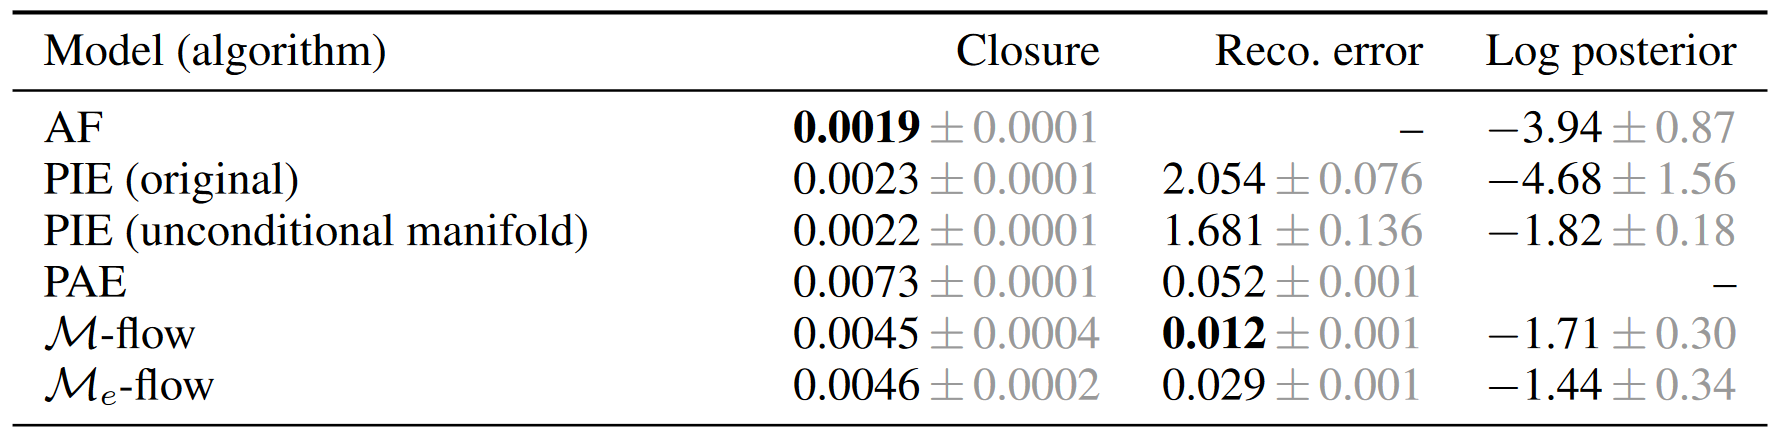
\includegraphics[width=0.9\linewidth]{chapters/petr_mokrov_s1/figs/particle_physics_res.png}
\end{figure}

\sunset{Closure} - тесты корректности генеративной модели; \sunset{Reco. error} - расстояние тестовой выборки до её проекции на выученное многообразие; \sunset{Log posterior} - правдоподобие истинного $\zeta^*$ на posterior KDE, построенного по MCMC.




\section{Questions To Discussion}
\begin{enumerate}
    \item Почему обычные потоки (AF) плохо оценивают плотность при моделировании данных на многообразиях?
    \item Какие вычислительные проблемы возникают у Rectangular flows ($\cM, \cM_e$ - flows) при оценке плотности?
    \item Каким образом можно спроецировать точку на многообразие, моделируемое $\cM$-потоком?
    \item В чём отличие между $\cM$ и $\cM_{e}$ потоками?
    \item Каким образом удаётся избежать сложных вычислений при семплировании из апостериорного распределения на параметрах модели с использованием MCMC в задаче simulation-based inference?
\end{enumerate}
    
    \clearpage
    \chapter{Forward and Backward Fourier transform and iPhone LiDAR imaging analysis}
    \section{Introduction}

Глава посвящена преобразованиям Фурье, некоторым их свойствам и ключевым применениям в теории обработки сигналов. В частности, рассматриваются приложения в задачах фильтрации одномерных и двумерных сигналов, Фурье-спектроскопии, формировании признакового описания входного сигнала.

\section{References Review}

\begin{itemize}
    \item ~\cite{MITcourse} -- открытый курс MIT, отдельные лекции которого посвящены преобразованиям Фурье и их приложениям в анализе сигналов;
    \item ~\cite{GonzalezWoods} -- источник, содержащий информацию об анализе и обработке изображений, в частности о применении преобразования Фурье для фильтрации изображений;
    \item ~\cite{LiDAR1, LiDAR2} -- работы, описывающее применение преобразования Фурье к сигналу LiDAR для построения признакового описания объекта;
\end{itemize}

\section{Main Part}

\subsection{Связь преобразований Фурье с рядом Фурье}

Для того, чтобы ввести преобразование Фурье, предлагается рассмотреть ряд Фурье для апериодической функции как предел ее периодического обобщения, тем самым на простом примере показать связь преобразования Фурье с рядами Фурье. Это рассуждение не является строгим доказательством, а лишь некоторой интуицией о связи понятий.

Здесь и далее сигнал понимается математически как функция одной или нескольких независимых величин.

Известно, что любой периодический сигнал может быть представлен в виде своего ряда Фурье. 
Теперь же рассмотрим некоторый апериодический сигнал, например, простой импульс $x(t) = \mathbb{I}(t \in [-S, S])$. 
\begin{figure}[!htb]
\center{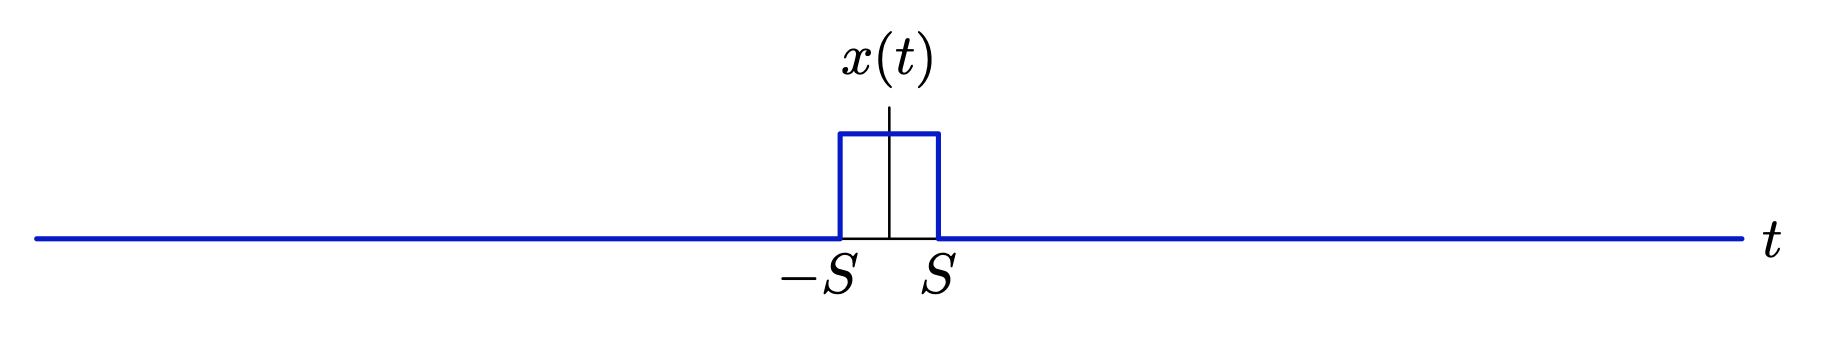
\includegraphics[width=0.7\textwidth]{chapters/grigorev_s1/pictures/xt}}
\caption{Апериодический сигнал $x(t)$}
\end{figure}

Апериодический сигнал может рассматриваться как периодический с бесконечным периодом.
Видоизменим сигнал $x(t)$, сделав его переодическим, просто сдвигая импульс на значение периода и суммируя:
$$x_T(t) = \sum \limits _{k=-\infty}^{\infty} x(t+kT) .$$
\begin{figure}[!htb]
\center{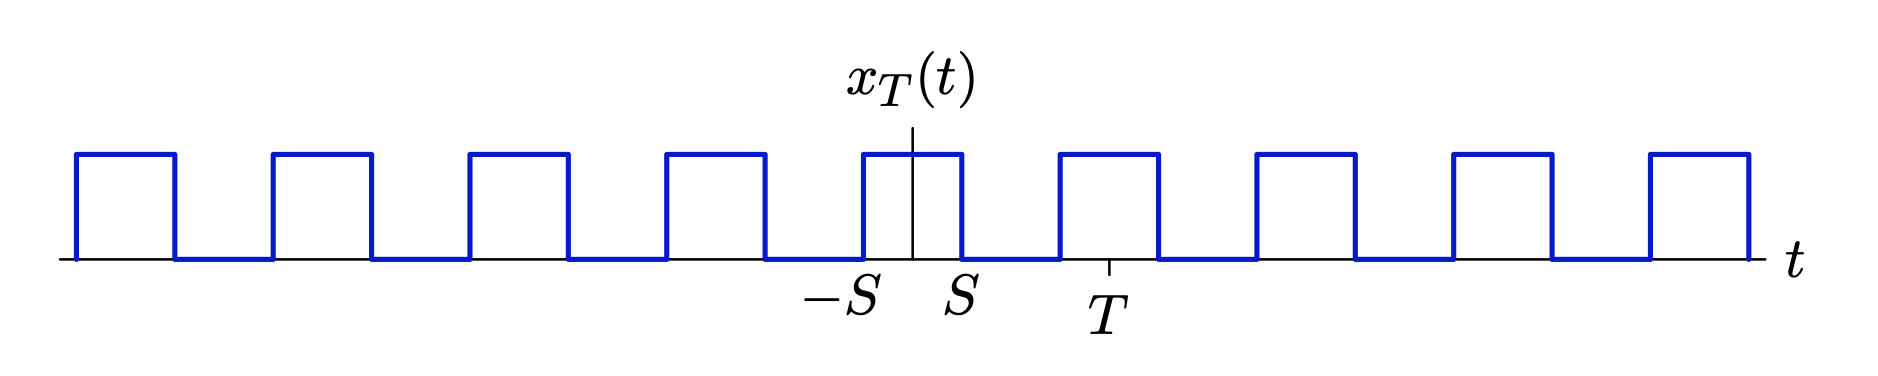
\includegraphics[width=0.7\textwidth]{chapters/grigorev_s1/pictures/xtt}}
\caption{Периодический обобщение $x_T(t)$ исходного сигнала $x(t)$}
\end{figure}

Сигнал, очевидно, периодический и, более того, предел такого периодического обобщения при $T\to \infty$ равен исходному сигналу:
$$x(t) = \lim \limits _{T \to \infty} x_T(t).$$

Дальнейшая идея состоит в том, чтобы попробовать разложить в ряд Фурье периодическое обобщение $x_T(t)$ исходного сигнала и перейти к пределу по $T$ для того, чтобы сделать некоторые выводы о таком преобразовании.

Периодическое обобщение $x_T(t)$ раскладывается в ряд Фурье, коэффициенты ряда Фурье для периодического сигнала выглядят следующим образом:
$$a_k = \frac{1}{T} \int \limits_{-T/2}^{T/2} x_T(t) e^{-i \frac{2\pi}{T}kt} dt = \frac{1}{T} \int \limits_{-S}^{S} e^{-i \frac{2\pi}{T}kt} dt = \frac{2}{T} \frac{\sin(\omega S)}{\omega}.$$
\begin{figure}[!htb]
\center{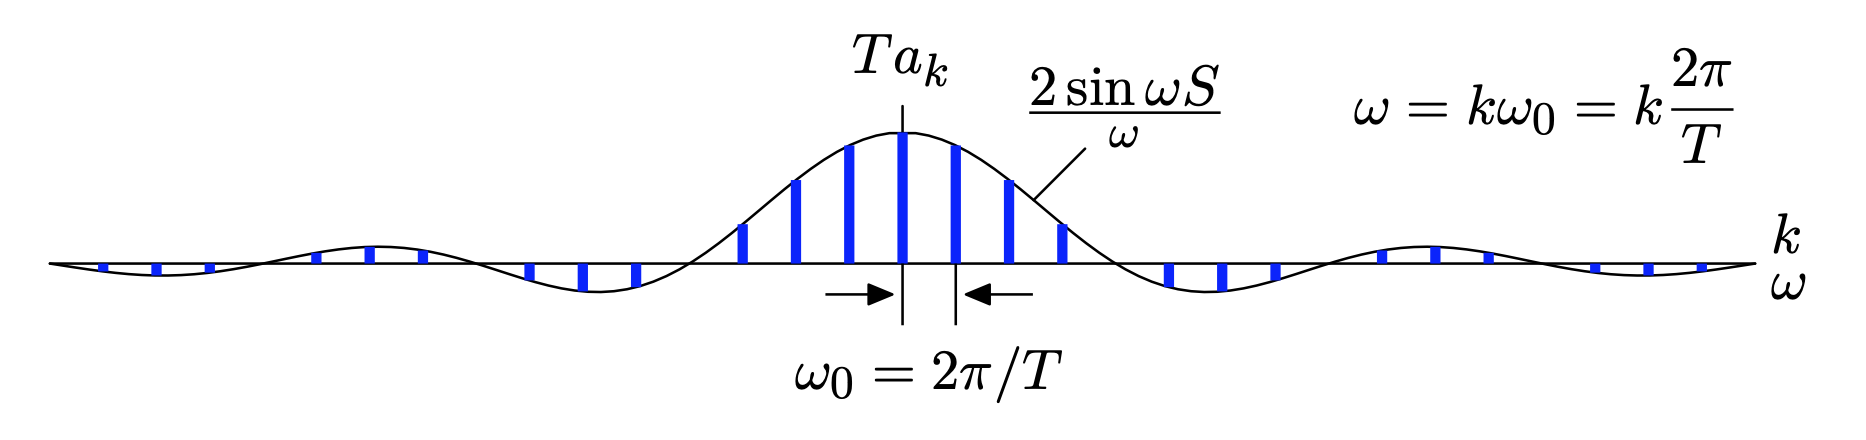
\includegraphics[width=0.7\textwidth]{chapters/grigorev_s1/pictures/tak}}
\caption{График зависимости $T a_k = f(k)$ и профиль амплитуд $E(\omega)$}
\end{figure}

Рассмотрим зависимость коэффициентов Фурье, масштабированных на значение периода, как функцию от номера $k$. Заметим, что увеличение периода вдвое приводит к тому, что огибающая не изменяется, но число коэффициентов, находящихся в заданном интервале частот $\omega$, увеличится вдвое. И в пределе величина $T a_k$ стремится к непрерывной функции $E(\omega)$, которая описывает профиль амплитуд:
$$\lim \limits_{T\to \infty}T a_k = \lim \limits_{T\to \infty} \frac{1}{T} \int \limits_{-T/2}^{T/2} x(t) e^{-i \frac{2\pi}{T}kt} dt = \frac{2}{T} \frac{\sin(\omega S)}{\omega} = E(\omega).$$
Причем функции $E(\omega)$ не зависит от $T$.

В обратную сторону, используя предельный переход к разложению периодического сигнала в ряд Фурье, можно получить представление исходного сигнала через интеграл от функции $E(\omega)$, домноженной на комплексный вес:
\begin{align*} 
x(t) & = \lim \limits _{T \to \infty} x_T(t) = \lim \limits _{T \to \infty} \sum \limits_{k=-\infty}^{\infty} \frac{1}{T} E(\omega) E^{i \frac{2 \pi}{T}kt} = \\
& =  \lim \limits _{T \to \infty} \sum \limits_{k=-\infty}^{\infty} \frac{\omega_0}{2 \pi} E(\omega) E^{i \omega t} = \frac{1}{2 \pi} \int \limits_{-\infty}^{\infty} E(\omega) e^{i \omega t} d \omega.
\end{align*}
Сумма здесь перешла в интеграл в Римановском плане. Таким образом, для простого сигнала получили преобразование Фурье. Проделанное не является выводом преобразования, а лишь описывает некоторую интуицию о связи ряда Фурье и преобразования Фурье.

\subsection{Преобразования Фурье}

Преобразование Фурье в общем случае имеет следующий вид:
$$X(i \omega) = \int \limits_{-\infty}^{\infty} x(t) e^{-i\omega t} dt.$$
Преобразование обратимо, обратное выглядит в меру симметрично:
$$x(t) = \frac{1}{2\pi} \int \limits_{-\infty}^{\infty} X(i \omega) e^{i \omega t} d\omega.$$
Преобразование Фурье обладает следующими характерными свойствами:
\begin{enumerate}
\item линейность: $a \, x_1(t) + b \, x_2(t) = a\,X_1(i \omega) + b\,X_2(i \omega)$;
\item сдвиг времени: $x(t - t_0) = e^{- i \omega t_0} X(i \omega)$;
\item масштабирование времени: $x(at) = \frac{1}{|a|}X(\frac{i \omega}{a})$;
\item дифференцирование: $\frac{dx(t)}{dt} = i \omega X(i \omega)$;
\end{enumerate}

\subsection{Дискретные преобразования Фурье}

На практике часто приходится иметь дело с сигналами, которые известны в конечном наборе точек $t \in [0, N-1]$, то есть дискретными. Будь это дискретность по времени или пространству не столь важно. Важно, чтобы шаг между точками, соответствующими наблюдаемым значениям, был равномерен.

Пусть $x(t) ~-$ исходный входной сигнал,  $t \in [0, N-1]$, $\{x_n\}_{n=0}^{N-1} ~-$ входной сигнал в дискретных временных точках $n=0,\dots,N-1$ c постоянным временем сэмплирования $dt=1$, то есть дискретный сигнал задает ступенчатую аппроксимацию $x(t)$.
Дискретное преобразования Фурье для данного сигнала можно получить из преобразования Фурье для функции, расписывая его для описанной дискретной аппроксимации, то есть для $N$ ступенек ширины $1$ с высотой, задаваемой дискретным сигналом:
\begin{align*}  
& X(i \omega) = \int \limits_{\infty}^{\infty} x(t) e^{-i\omega t} dt = \int \limits_{0}^{N-1} x(t) e^{-i\omega t} dt = \sum \limits _{n=0}^{N-1} x_n e^{-i \omega n},\\
& \omega=k \frac{2 \pi}{N}, \, k=0,\dots,N-1.
\end{align*}
Набор частот в данном случае определяется следующим образом. Очевидно, что число частот равно числу входных значений, чтобы на выходе размерность сохранялась. Остается заметить, что исходная дискретная аппроксимация задана на отрезке $[0, N]$ и может быть периодически продлена на оставшуюся ось с периодом $N$. Вспоминая о связи ряда Фурье и преобразования Фурье, получим набор частот $\omega=k \frac{2 \pi}{N}, \, k=0,\dots,N-1$. Данный набор частот может быть выбран иначе, например, симметрично относительно $0$ согласно формуле Эйлера.
Общий вид прямого и обратного дискретных преобразований Фурье выглядит следующим образом. Прямое дискретное преобразование Фурье \textit{(DFT)}: 
$$X_k = \sum \limits _{n=0}^{N-1} x_n e^{-i\frac{2 \pi}{N}kn}$$,
обратное дискретное преобразование Фурье \textit{(IDFT)}:
$$x_n = \frac{1}{N} \sum \limits _{k=0}^{N-1} X_k e^{i\frac{2 \pi}{N}kn}.$$ 

Заметим, что дискретное преобразование Фурье можно представить в матричном виде. Исходный дискретный сигнал запишется в виде столбца, коэффициенты из комплексных экспонент образуют матрицу. Преобразование — умножение матрицы на столбец, то есть $N^2$ операций умножения.  Тогда сложность, соответствующая наивному алгоритму равна $O(N^2)$. Существует более эффективный алгоритм со сложностью $O(N \log N)$, принимающий во внимание структуру задачи. Данный алгоритм известен как быстрое преобразование Фурье. Алгоритмы синонимичны, зачастую когда говорят, что используется DFT, то подразумевается вычисление именно FFT.

Далее будут упомянуты некоторые приложения преобразований Фурье в анализе сигналов. 

\subsection{Фурье фильтрация}

Пожалуй, одно из основных применений преобразования Фурье — это фильтрация сигнала. Зачастую шум, который мы хотим отфильтровать от исходного сигнала, представляет собой высокочастотные или низкочастотное колебания. Очевидно, что наиболее удобно в данном случае производить фильтрацию сигнала по частотному спектру. Общая процедура заключается в применении преобразования Фурье к исходному сигнала $x(t)$, наложению фильтра $H(\omega)$ на выделенный спектр $X(\omega)$ и применении обратного преобразования Фурье для получения отфильтрованного сигнала $y(t)$.
\begin{figure}[!htb]
\centering
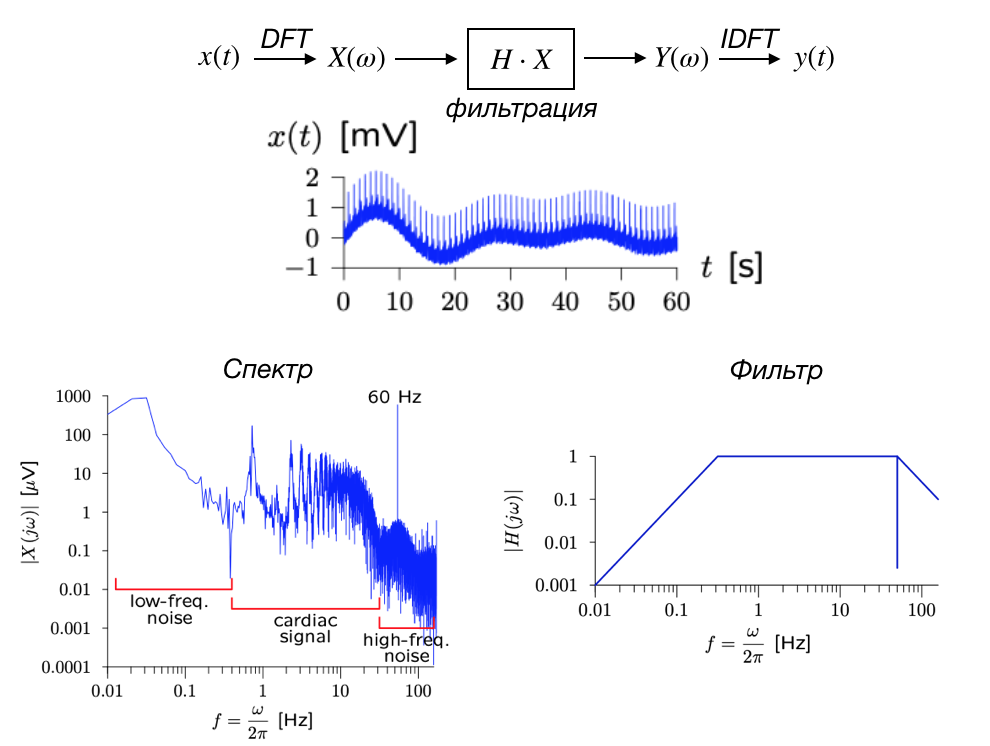
\includegraphics[width=16cm]{chapters/grigorev_s1/pictures/s6}%
\caption{Схема фильтрации электрокардиограммы}
\end{figure}

Растровое изображение тоже является сигналом как функция яркости $f(x, y)$ от координат пикселя $x=0,\dots,N-1$, $y=0,\dots,N-1$. Зачастую изображения содержат периодический высокочастотный шум, который требуется отфильтровать.

Двумерное преобразование Фурье выглядит следующим образом:
$$F(\omega_x, \omega_y) = \sum \limits _{x=0}^{N-1} \sum \limits _{y=0}^{N-1} f(x, y) e^{-i (\omega_x x + \omega_y y)}.$$
Частоты $\omega_x$ и $\omega_y$ определяются аналогично одномерному случаю, таким образом, они  принимают следующие $N$ значений:
$$\omega_x, \omega_y \in \left\{ k \frac{2 \pi}{N} \Bigg| k=0,\dots,N-1 \right\} .$$
На практике удобно сдвинуть часть частот на $2 \pi$, что допустимо по формуле Эйлера, сделав частоты симметричными по отношению к $0$ с шагом $\frac{2 \pi}{N}$.

Результат преобразование Фурье входного изображения представляет собой комплекснозначное изображение. Комплекснозначное изображение описывается амплитудами и фазами, как правило для фильтрации шума достаточно анализа изображения, соответствующего амплитудам спектра.
Таким образом, для частотного спектра производится фильтрация высокочастотных пиков амплитуд, соответствующих шуму и применяется обратное преобразование Фурье для получения отфильтрованной картинки.
\begin{figure}[!htb]
\centering
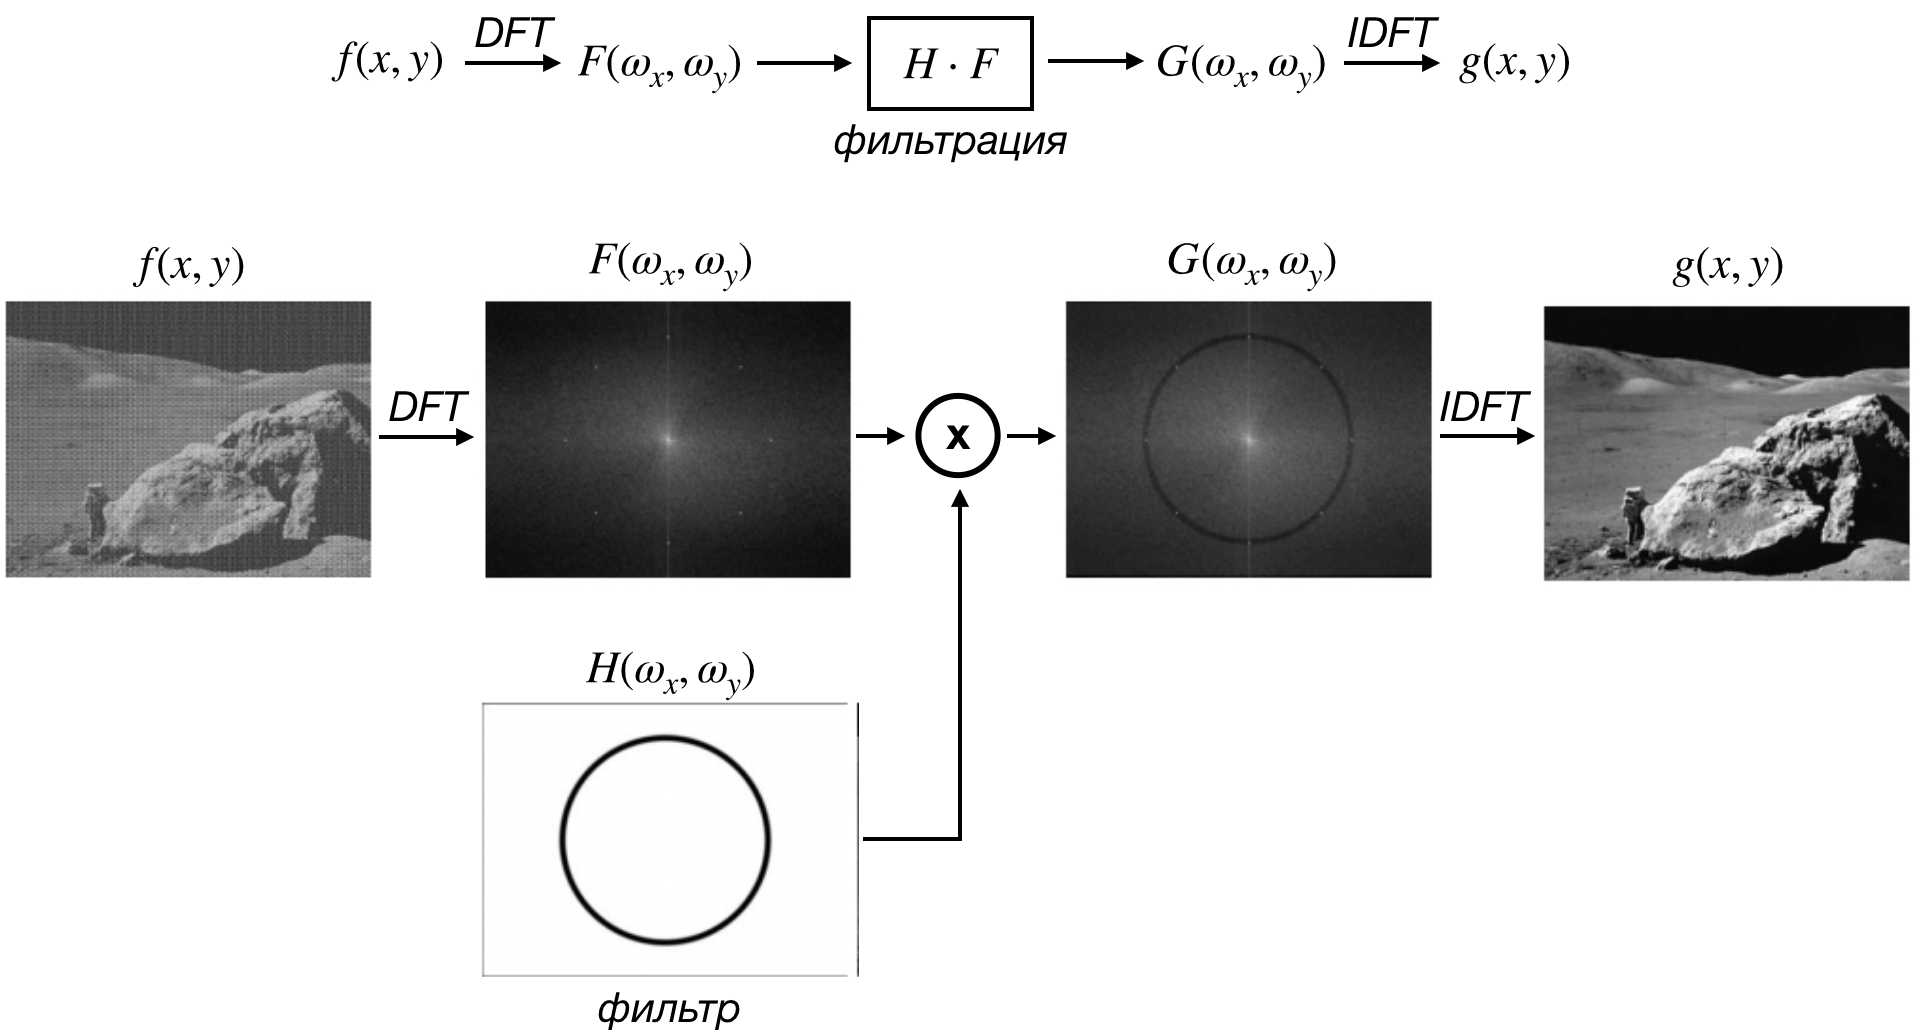
\includegraphics[width=16cm]{chapters/grigorev_s1/pictures/image_filtartion_with_scheme}%
\caption{Схема фильтрации изображения}
\end{figure}

\newpage
\subsection{Фурье спектроскопия}

Преобразование Фурье находит свои применения и в физике, в частности в оптике. Задача спектроскопии — определение спектра излучения некоторого источника, в общем случае немонохроматического.
Интерферометр Майкельсона $~-$ основа Фурье-спектроскопии, прибор позволяет определить спектр излучения по интерференционной картине.
\begin{figure}[!htb]
\centering
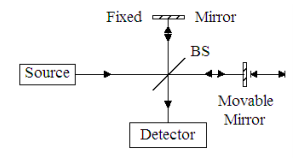
\includegraphics[width=8cm]{chapters/grigorev_s1/pictures/interferometer}%
\caption{Схема интерферометра Майкельсона}
\end{figure}
Здесь можно рассмотреть два случая — монохроматический и немонохроматический источник. В первом случае зависимость интенсивности от геометрической разности хода имеет следующий вид:
$$I(\delta) = \frac{1}{2} \left[ \cos\left( \frac{2 \pi \delta}{\lambda} \right) + 1 \right],$$ 
где $\delta ~-$ разность хода, $\lambda ~- $ длина волны. В данном случае параметр длины волны $\lambda$ находится аналитически, например, через первый минимум интенсивности.
В немонохроматическом случае суммируются интенсивности от всех длин волн:
$$I(\delta) = \sum \limits _j \frac{1}{2} \left[ \cos\left( \frac{2 \pi \delta}{\lambda_j} \right) + 1 \right],$$ 
аналитически спектр не найти. Однако в данном случае спектр излучения источника можно получить через преобразование Фурье полученной спектрограммы. 
\begin{figure}[!htb]
\centering
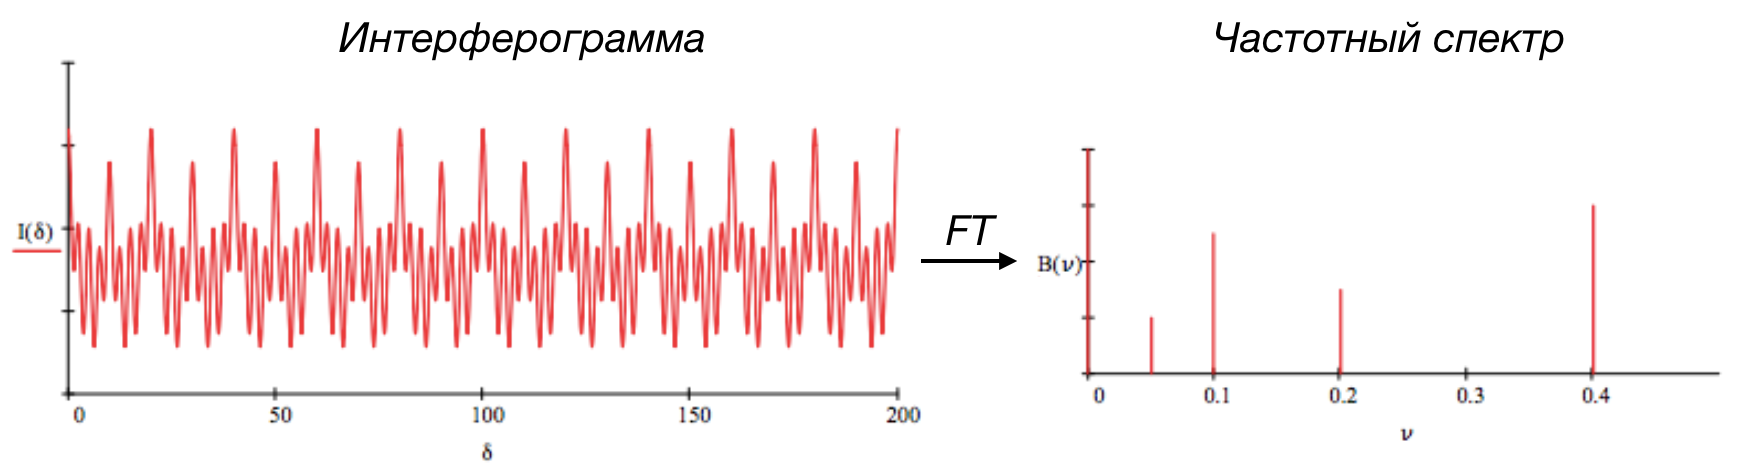
\includegraphics[width=14cm]{chapters/grigorev_s1/pictures/interferogram_spectrum}
\caption{Схема определения спектра излучения по интерферограмме}
\end{figure}

\subsection{Преобразования Фурье в LiDAR}

Последнее применение преобразование Фурье, которое будет освещено в данном семинаре, связано с построением признакового пространства в задачах, где исходные данные представляют собой временной ряд. Данное применение рассматривается на примере LiDAR, метода измерения расстояния до объекта. Базовый физический принцип прибора тривиален, расстояние вычисляется через время возврата волны (лазера) с известней скоростью распространения (скоростью света).
\begin{figure}[!tb]
\centering
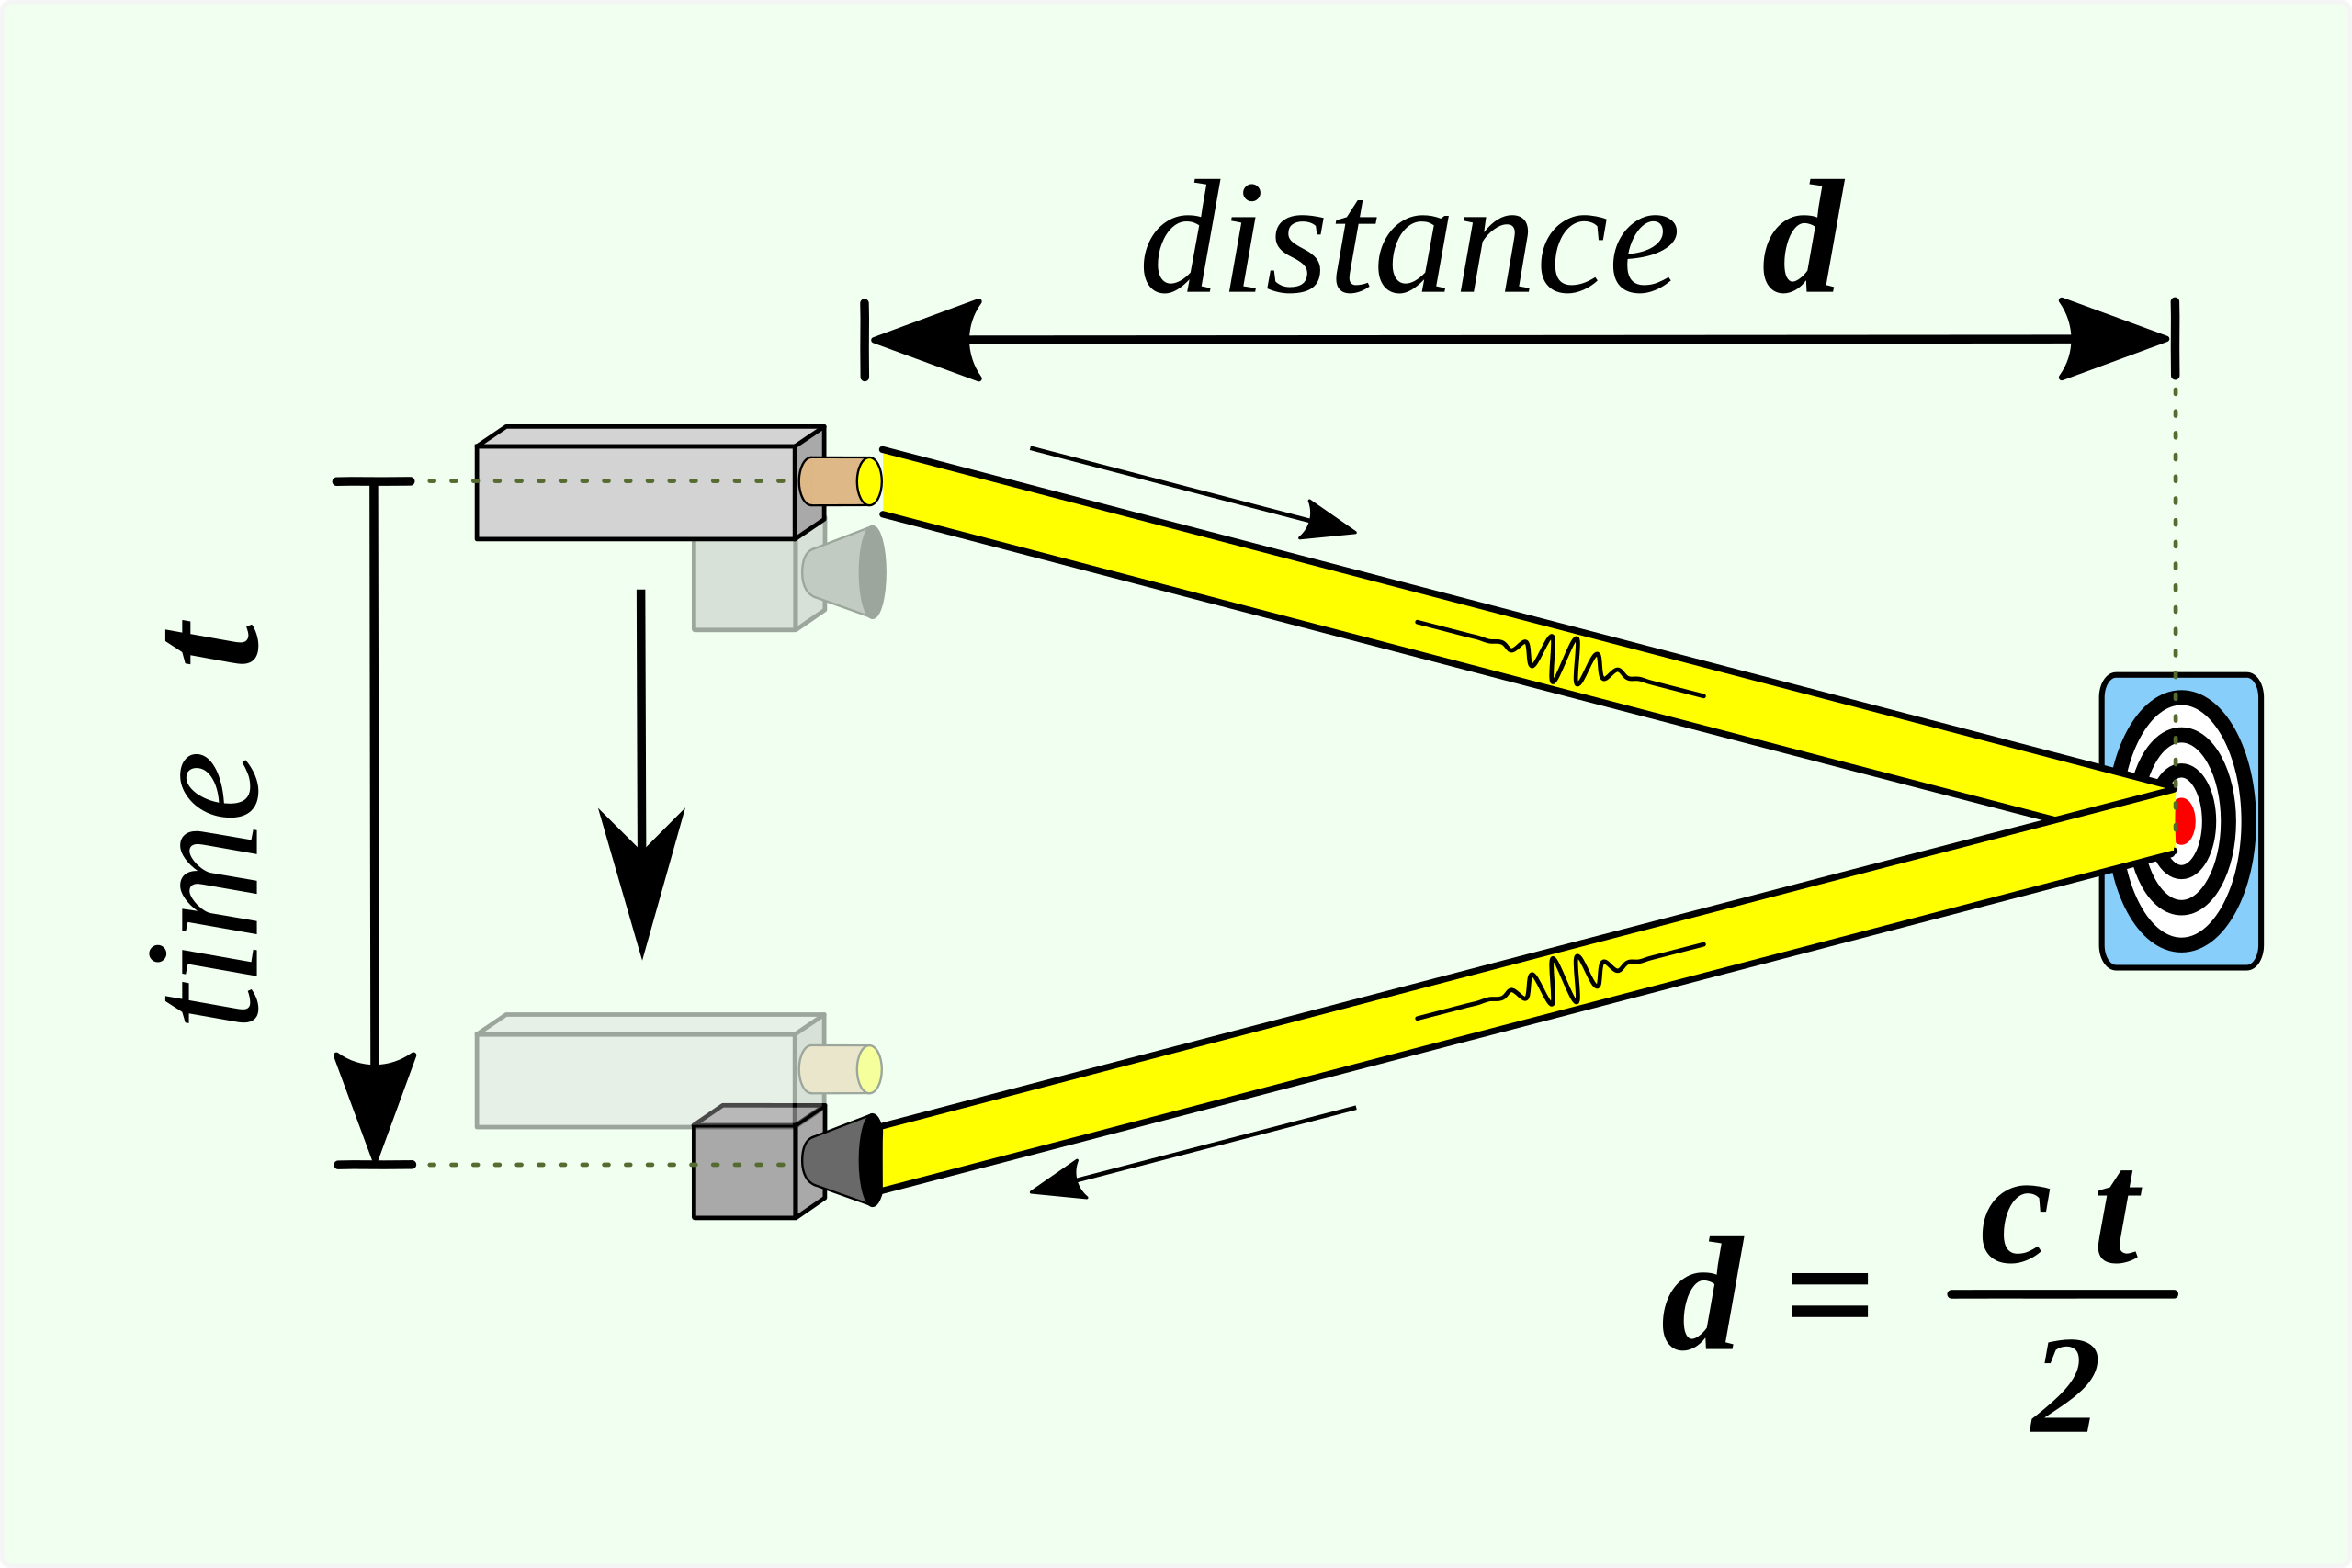
\includegraphics[width=6cm]{chapters/grigorev_s1/pictures/lidar_scheme}%
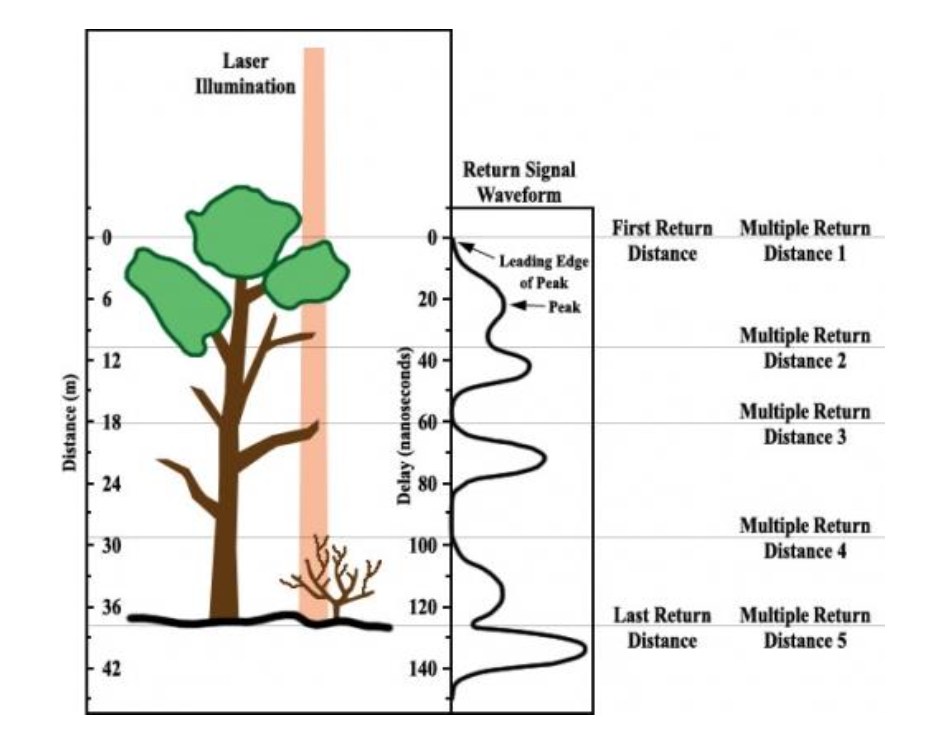
\includegraphics[width=6cm]{chapters/grigorev_s1/pictures/lidar}%
\caption{Схема LiDAR и регистрируемый сигнал}
\end{figure}

Как правило статьи, связанные с практическим применением LiDAR, имеют следующее применение преобразования Фурье вне зависимости от решаемой задачи машинного обучения. Применение состоит в формировании признакового пространства для алгоритма машинного обучения путем применения DFT к LiDAR сигналу. Объект — временной ряд $\{x_n\}_{n=0}^{N-1}$ амплитуд отраженного от поверхности сигнала. Для данного временного ряда вычисляется DFT, $\{X_k\}_{k=0}^{N-1} ~- $ сигнал после DFT, используемый в качестве признакового описания сигнала. В силу того, что данные величины комплекснозначны $\forall k = 0, \dots, N-1 \,\,\,\, X_k \in \mathbb{C}$, их удобно описывать через амплитуду и фазу соответственно. Остается уточнить, что для действительнозначного сигнала (а временной ряд амплитуд действительнозначен) использование всех значений, полученных в результате применения DFT, избыточно в силу свойства DFT для действительнозначного входного сигнала: $X_k = \overline{X_{N-k}} \,\, \forall k$. Таким образом, итоговое признаковое описание сигнала задается амплитудами и фазами половины значений DFT.

\section{Questions To Discussion}

\begin{enumerate}
\item В чем заключается логическая связь между рядами Фурье и преобразованием Фурье? 
\item Алгоритмическая сложность DFT и FFT?
\item Основное применение преобразование Фурье в анализе сигналов?
\item Чему соответствует центральная точка изображения, представляющего амплитуды образа DFT исходной картинки? 
\item Чему равна эффективная размерность признакового пространства, полученного применением DFT к действительнозначному временному ряду длины $T$, как формируется это признаковое пространство?
\end{enumerate}
    
    \clearpage
    \chapter{Spectral analysis on meshes}
    \section{Introduction}

Глава посвящена спектральному анализу решеток, в частности общей схеме спектрального анализа, базовым понятиям, теоретическим основам и возможным применениям для решения прикладных задач.

\section{References Review}

\begin{itemize}
    \item ~\cite{GDL} -- основная работа курса, глава которой содержит краткую обзорную информацию о методологии спектрального анализа решеток;
    \item ~\cite{SpectralMeshSurvey} -- наиболее полная обзорная статья, посвященная спектральному анализу решеток и стандартизации существующих подходов в данной области;
    \item ~\cite{SpectralMeshSurvey2} -- обзор существующих подходов к спектральному анализу решеток с математическим обоснованием (частично дублирует \cite{SpectralMeshSurvey});
    \item ~\cite{SpectralMeshSurveyCourse} -- семинар-практикум по спектральному анализу графов и решеток;
\end{itemize}

\section{Main Part}

Определим понятие треугольной решетки. 
\textit{Треугольная решетка} $\mathcal{M}$ -- ненаправленный граф с дополнительной структурой, то есть пара вида $(\mathcal{G}, \vect{P})$, где
	\begin{itemize} 
		\item $\mathcal{G} = (\mathcal{V}, \mathcal{E}) ~- $ граф, 
		\item $\mathcal{V} ~-$ множество вершин графа, 
		\item $\mathcal{E} \subset \mathcal{V} \times \mathcal{V} ~-$ множество ребер графа, 
		\item $\vect{P} = \left[ \vect{p}_1 \, \dots \vect{p}_n \right] \in \mathbb{R}^{n \times 3} ~- $ матрица трехмерных координат вершин решетки, то есть
		$\vect{p}_i = [x_i, y_i,z_i] ~-$ координаты вершины $i \in \mathcal{V}$. 
	\end{itemize}
Примером треугольной решетки может послужить триангуляция некоторой трехмерной фигуры.

\begin{figure}[!htb]
\center{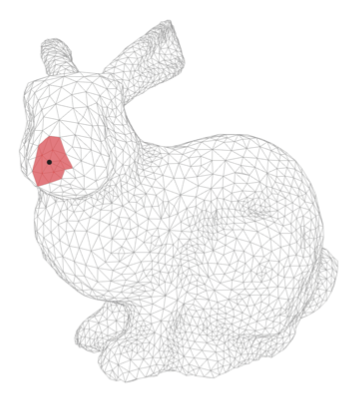
\includegraphics[width=5cm]{chapters/grigorev_s2/pictures/mesh_ex}}
\caption{Пример графовой решетки}
\end{figure}

\subsection{Лапласиан решетки}

Далее речь пойдет о спектральном анализе решеток. Большинство методов спектрального анализа имеют схожую схему, которая может быть обобщена следующим образом. В спектральном анализе предполагается $3$ основных этапа. На первом для заданной решетки определяется некоторый линейный оператор $\vect{M}$, элементы $M_{ij}$ которого соответствует информации о связи вершин $i$ и $j$. В частности $M_{ij}$ может нести информацию о смежности или относительном геометрическом расположении вершин $i$ и $j$ по отношению друг к другу. На втором этапе для определенного линейного оператора $\vect{M}$, заданного в матричном виде, вычисляются собственные числа и собственные вектора. В последствии производится анализ собственных чисел и собственных векторов оператора $\vect{M}$ с целью решение поставленной задачи.

Одним из вариантов выбора оператора $\vect{M}$ является комбинаторный лапласиан.
Комбинаторный лапласиан решетки $\mathcal{M} = (\mathcal{G}, \vect{P})$ полностью определяется ее графом $\mathcal{G} = (\mathcal{V}, \mathcal{E})$. Пусть $\vect{W} ~-$ матрица смежности графа $\mathcal{G}$, то есть 
		\begin{equation*}
		W_{ij} = 
		 \begin{cases}
   		1 &\text{если $(i,j) \in \mathcal{E}$,}\\
   		0 &\text{иначе.}
		 \end{cases}
		\end{equation*}
дополнительно вводится матрица $\vect{D}$ (\textit{degree matrix}) как 
		\begin{equation*}
		D_{ij} = 
		 \begin{cases}
   		d_i = |N(i)|&\text{если $i=j$,}\\
   		0 &\text{иначе,}
		 \end{cases}
		\end{equation*}
где $d_i ~-$ степень вершины $i \in \mathcal{V}$. Тогда комбинаторный лапласиан $\vect{K}$ (\textit{матрица Кирхгофа}) определяется как
		\begin{equation*}
		\vect{K} = \vect{D} -\vect{W}.
		\end{equation*}
Таким образом, комбинаторный лапласиан $\vect{K}$ содержит информацию о локальных свойствах решетки: смежности вершин и их степени. Геометрическая информация, о расположении вершин решетки, не используется для определения комбинаторного лапласиана.

Для комбинаторного лапласиана можно показать связь с оператором Лапласа-Бельтрами в случае риманова многообразия, в частности комбинаторный лапласиан является естественным обобщением данного оператора для решетки.
Оператор Лапласа-Бельтрами на римановом многообразии, действующий на гладкую функцию $\phi$: 
	$$\Delta(\phi) = \text{div}\, (\text{grad}(\phi)).$$
Пусть $\mathcal{G} = (\mathcal{V}, \mathcal{E}) ~-$ граф триангуляции данного риманова многообразия, а $f : \mathcal{V} \to \mathbb{R} ~- $ сужение функции $\phi$ на $\mathcal{V}$.
Определим ориентированную матрицу инцидентности $\vect{R} \in \mathbb{R}^{n \times m}$ графа $\mathcal{G}$, ориентация ребер которого задана произвольно:
	\begin{equation*}
		R_{ie} = 
		 \begin{cases}
   		-1 &\text{если $i \in \mathcal{V} ~-$ начальная вершина ребра $e \in \mathcal{E}$,}\\
   		+1 &\text{если $i \in \mathcal{V} ~-$ конечная вершина ребра $e \in \mathcal{E}$.}
		 \end{cases}
	\end{equation*}
Несложно заметить связь комбинаторного лапласиана и ориентированной матрицы инцидентности: $$\vect{K} = \vect{R} \vect{R}^T.$$
Тогда оператор $\vect{R}^T f : \hat{\mathcal{E}} \to \mathbb{R} $ действует на множестве направленных ребер $\hat{\mathcal{E}}: \,\, | \hat{\mathcal{E}}| = 2 |\mathcal{E}|$:
	$$(\vect{R}^T f)(e) = f(e^+) - f(e^-),$$
где $e^-, \, e^+ ~-$ начальная и конечная вершины ребра $e$ соответственно. 
	
Величина $(\vect{R}^T f)(e)$ может рассматривать как естественный аналог градиента функции $\phi$ на ребре $e$, тогда оператор $\vect{K} = \vect{R} \vect{R}^T $ соответствует дивергенции градиента. Таким образом, комбинаторный лапласиан решетки -- дискретный аналог оператора Лапласа-Бельтрами. При измельчении размера триангуляции в пределе комбинаторный лапласиан соответсвует непрерывному оператору Лапласа-Бельтрами.

\subsection{Спектр лапласиана}

Свойства комбинаторного лапласиана позволяют в некоторой степени описать его спектр. В частности для комбинаторного лапласиана выполнена спектральная теорема, поскольку лапласиан является симметричной положительно полуопределенной матрицей. \medskip

\textbf{Cпектральная теорема}

Пусть $\vect{S} \in \mathbb{R}^{n \times n} ~- $ действительнозначная симметричная матрица, тогда ее спектральное разложение:
$$\vect{S} = \vect{V}  \bm{\Lambda} \vect{V}^T = \sum \lambda_i \vect{v}_i \vect{v}_i^T,$$ 
где $\vect{V} = [\vect{v}_1 \, \dots \, \vect{v}_n] ~- $  матрица, составленная из собственных векторов матрицы $\vect{S}$, $ \bm{\Lambda} ~-$ диагональная матрица из собственных значений матрицы $\vect{S}$. Причем собственные значения действительный, а собственные вектора ортогональны.

Из положительной полуопределенности комбинаторного лапласиана следует, что его собственные значения неотрицательны. В частности комбинаторный лапласиан вырожден, его наименьшее собственное значение равно $0$, кратность данного собственного значения равна числу компонент связности графа, то есть для решетки кратность в общем случае равна $1$. Собственные вектора лапласиана ортогональны.

\begin{figure}[!htb]
\center{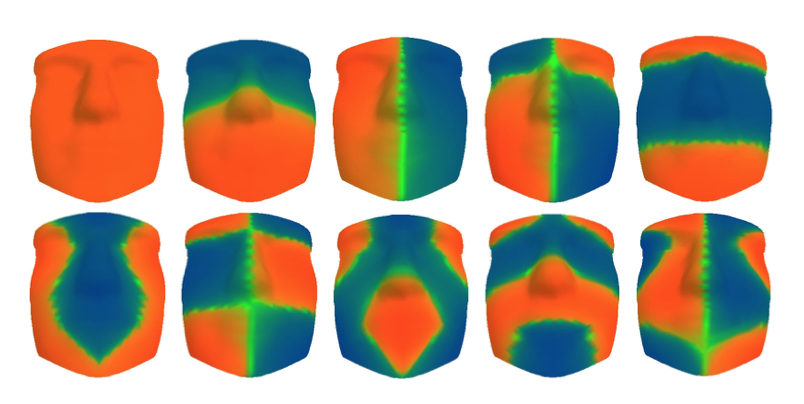
\includegraphics[width=10cm]{chapters/grigorev_s2/pictures/face_mesh}}
\caption{Визуализация первых $10$ собственных векторов лапласиана решетки лица}
\end{figure}

\subsection{Спектральное преобразование}

Ортогональность собственных векторов комбинаторного лапласиана позволяет рассматривать их как аналог Фурье базиса.  Обратное дискретное преобразование Фурье соответствует разложению исходного сигнала по ортогональному базису 
	$$\vect{x} = \sum \limits _{k=0}^{n-1} y_k \bm{\psi}_k = \bm{\Psi} \vect{y},$$ 
где $\{ \bm{\psi}_k\}_{k=0}^{n-1} ~- $ базис Фурье, $\vect{x} ~- $ исходный сигнал, $\vect{y} ~- $ его Фурье образ.
Собственные вектора $\vect{v}_1 \, \dots \, \vect{v}_n$ лапласиана $\vect{K}$ образуют аналог базиса Фурье, соответствующие им собственные значения рассматриваются как частоты.
На практике собственные вектора подобны гармоникам.
Тогда может быть введено спектральное преобразование, подобное дискретному преобразованию Фурье, которое определяется через собственные вектора $\vect{v}_1 \, \dots \, \vect{v}_n$  \, ($\lambda_1 \le \dots \le \lambda_n$) лапласиана $K$:
	$$\vect{Y} = \vect{V}^T \vect{X},$$
где $\vect{V} = [\vect{v}_1 \, \dots \, \vect{v}_n]$, $\vect{X} \in \mathbb{R}^{n \times 3} ~- $ координатный сигнал на решетке, $\vect{Y} ~- $ образ.

Данное спектральное преобразование имеет общие свойства с преобразованием Фурье, из чего вытекают схожие применения, например, фильтрация сигнала на решетке.
В частности фильтрация координатного сигнала $x: \mathcal{V} \to \mathbb{R}^3$, $x(i)=\vect{p}_i$ на решетке $\mathcal{M}=(\mathcal{V}, \mathcal{E}, \vect{P})$ состоит в последовательном применении DFT-подобного спектрального преобразования, оператора фильтрации и обратного спектрального преобразования.
\begin{figure}[!htb]
\center{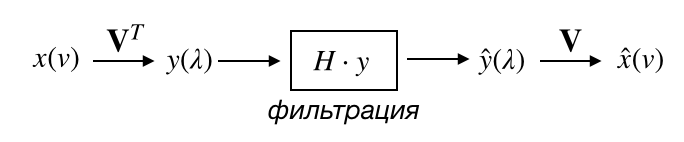
\includegraphics[width=10cm]{chapters/grigorev_s2/pictures/filtration_scheme}}
\caption{Схема фильтрации координатного сигнала}
\end{figure}
На практике зачастую выбирается фильтр нижних частот, пропускающий лишь компоненты, отвечающие меньшим собственным значениям лапласиана $\vect{K}$, которые в данном случае рассматриваются в качестве частот.
Частным случаем спектральной фильтрации является спектральная компрессия -- фильтрация с идеальным фильтром низких частот, то есть пропускающим лишь $k$ наименьших частот спектра.

\begin{figure}[!htb]
\center{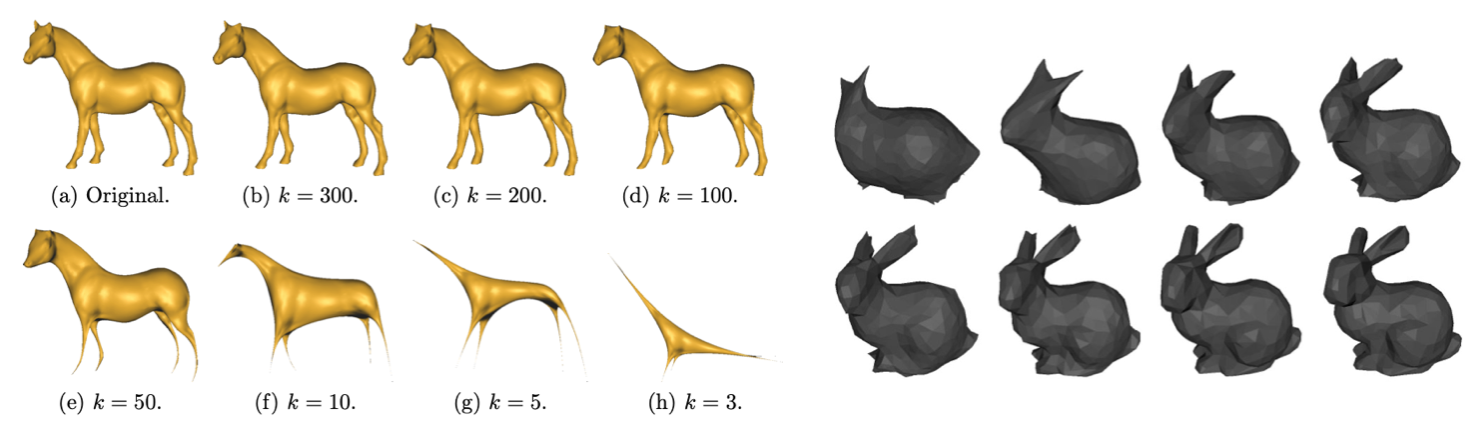
\includegraphics[width=14cm]{chapters/grigorev_s2/pictures/rabbit_horse_mesh}}
\caption{Примеры восстановления решеток с применением спектральной компрессии}
\end{figure}

\subsection{Cпектральный дескриптор}

Лапласиан $\vect{K}$ решетки описывает локальную информацию о ее структуре: смежность вершин и их степень, однако согласно спектральной теории графов собственные значения и собственные векторы лапласиана $\vect{K}$ несут значимую (достаточно полную) глобальную информацию о решетке.  В связи с этим во многих практических приложениях для решения задач используется не сам комбинаторный лапласиан, а спектральный дескриптор, определяющийся через собственные значения и собственные векторы комбинаторного лапласиана и представляющий собой эмбеддинг, сохраняющий полную информацию о лапласиане.
Для спектрального разложения $\vect{K} = \vect{V}  \bm{\Lambda} \vect{V}^T $ лапласиана $\vect{K}$ заданной решетки $\mathcal{M}$ спектральный дескриптор определяется как:
	$$\vect{W} = \vect{V} \bm{\Lambda}^{1/2},$$
спектральный дескриптор полностью описывает лапласиан $\vect{K} = \vect{W} \vect{W}^T$.

Использование полного спектрального дескриптора $\vect{W}$ осложняется его высокой размерность, в связи с этим требуется производить снижение размерности дескриптора для его эффективного применения.
Оптимальный метод снижения размерности спектрального дескриптора $\vect{W}$ описывается следующей теоремой.\medskip

\textbf{Теорема (\textit{Eckart-Young})}
\begin{itemize}
\item $\vect{S} \in \mathbb{R}^{n \times n} ~- $ действительнозначная симметричная положительно полуопределенная матрица, ее спектральное разложение $\vect{S} = \vect{V}  \bm{\Lambda} \vect{V}^T $. Собственные значения на диагонали матрицы $\bm{\Lambda}$ расположены по убыванию. 
\item $\vect{W} = \vect{V} \bm{\Lambda}^{1/2} ~-$ матрица собственных векторов, масштабированных на корень соответствующих собственных значений.
\item $\vect{W}_{(k)} \in \mathbb{R}^{n \times k} ~- $ усеченная матрица $\vect{W}$, состоящая из $k$ первых столбцов $\vect{W}$.
\item $\vect{W}_{(k)} \vect{W}_{(k)}^T ~-$ лучшая в терминах нормы Фробениуса аппроксимация ранга $k$ для матрицы $\vect{S}$:
$$\vect{W}_{(k)} = \arg \min \limits _{\substack{\vect{U} \in \mathbb{R}^{n \times k} \\ \text{rank}(\vect{U})=k}} \| \vect{S} - \vect{U} \vect{U}^T \|$$
\end{itemize}


Таким образом, уменьшение размерности спектрального дескриптора $\vect{W}$ выбором подматрицы $\vect{W}_{(k)}$, отвечающей $k$ наибольшим собственным значениям лапласиана $K$, оптимально с точки зрения сохранения информации.

\section{Questions To Discussion}
\begin{enumerate}
\item Чем заменить матрицу смежности в определении комбинаторного лапласиана, чтобы он учитывал геометрическую структуру (координаты) решетки?
\item Почему описанный лапласиан называется комбинаторным?
\item Как определить критерий выбора параметра $k$ (число частот после фильтрации) в спектральной компрессии? 
\item Чему равно наименьшее собственное значение и соответствующий собственный вектор комбинаторного лапласиана $\vect{K}$? Почему визуализация данного собственного значения отлична от остальных?
\end{enumerate}
    
    \clearpage
    \chapter{Tensor representation of the Brain Computer Interface}
    \section{Introduction}
При построении нейроинтерфейса обычно используются данные сигналов активности головного мозга, представленные в виде многомерных рядов со значениями напряжения на установленных электродах. 

\begin{figure}[h]
	\centering
	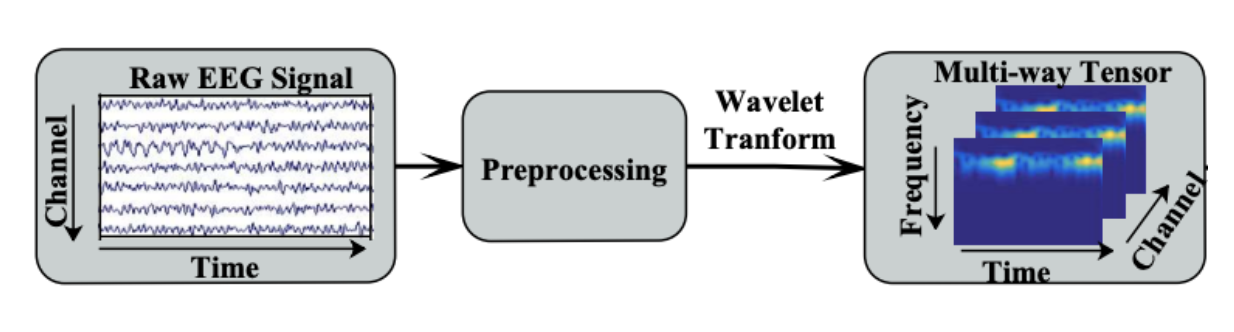
\includegraphics[width=0.9\textwidth]{chapters/varenik2/images/multi-way-eeg.png}
\end{figure}

Такие сигналы естественным образом часто имеют более двух доменов. К времени и пространству добавляется еще частота, получаемая после спектральной предобработки сигнала, помимо этого в одном эксперименте могут учавствовать различные группы испытуемых, использоваться разные условия формирования стимула  и проводиться множество попыток. Использование тензорного представление стало популярным инструментом при работе с биомедицинскими, химическими данными, при обработке сигналов и изображений из-за многомерной структуры таких данных. Поскольку их анализ в матричном виде часто приводит к потере важной информации о существующих связях между представлениями, что приводит к уменьшению полноты признакового описания и, следовательно, ухудшает производительность системы.

\section{References Review}
В книге~\cite{Kolda2009TensorDA} рассматриваются методы тензорного разложения и их применение. В частности, в ней приведены теоретические описания канонически полиадического разложения и расложения Таккера, описаны их свойства и методы вычисления. В статье~\cite{CONG201559} приводится обзор применения тензорного анализа для сигналов EEG, а также описывается обобщение PLS на высокоразмерные тензоры - NPLS с использованием  представления тензора объектов через канонически полиадическое разложение. 
Работа~\cite{6365194} посвящена разработке еще одного обобщения PLS на тензорный случай. В его основе лежит разложение Таккера в композии с канонически полиадическим разложением для обеспечения лучшей аппроксимации исходных данных и единственности разложения при введении условий ортогональности. 

\section{Main Part}
Рассмотрим для начала базовые методы тензорного разложения, такие как каноническое полиадическое разложение и разложение Таккера, которые являются обобщениями матричного SVD для тензорного случая. Они находят широкое применение при анализе многомерных данных в различных приложениях, а именно уменьшение размерности, извлечение и отбор признаков для построения устойчивой модели, анализ независимых компонент и полезны в интерпретации для обеспечения связей между извлеченными факторами и их физиологическими значениями.

\subsection{Канонически полиадическое разложение (CP decomposition)}

\textbf{3-way}

Рассмотрим для начала трехмерный случай, а потом обобщим на N-мерный.
Пусть $\vect X \in \mathbb{R}^{I\times J \times K}$ - тензор 3-го порядка. Каноническое полиадическое разложение $\vect X$ есть линейная комбинация тензоров единичного ранга (внешних произведений векторов):
\begin{gather}
    \vect X \approx [\bm{\lambda}; \vect A, \vect B, \vect C] \equiv \sum\limits_{r=1}^R \lambda_r \vect a_r \circ \vect b_r \circ \vect c_r, \text{ } \vect a_r \in \mathbb{R}^I, \vect b_r \in \mathbb{R}^J, \vect c_r \in \mathbb{R}^K, \lambda_r \in \mathbb{R},
    \label{eq1}
\end{gather}
$\vect A \in \mathbb{R}^{I\times R}, \vect B \in \mathbb{R}^{J\times R}, \vect C \in \mathbb{R}^{K\times R} - \text{фактор-матрицы}$.
	
\begin{figure}[h]
	\centering
	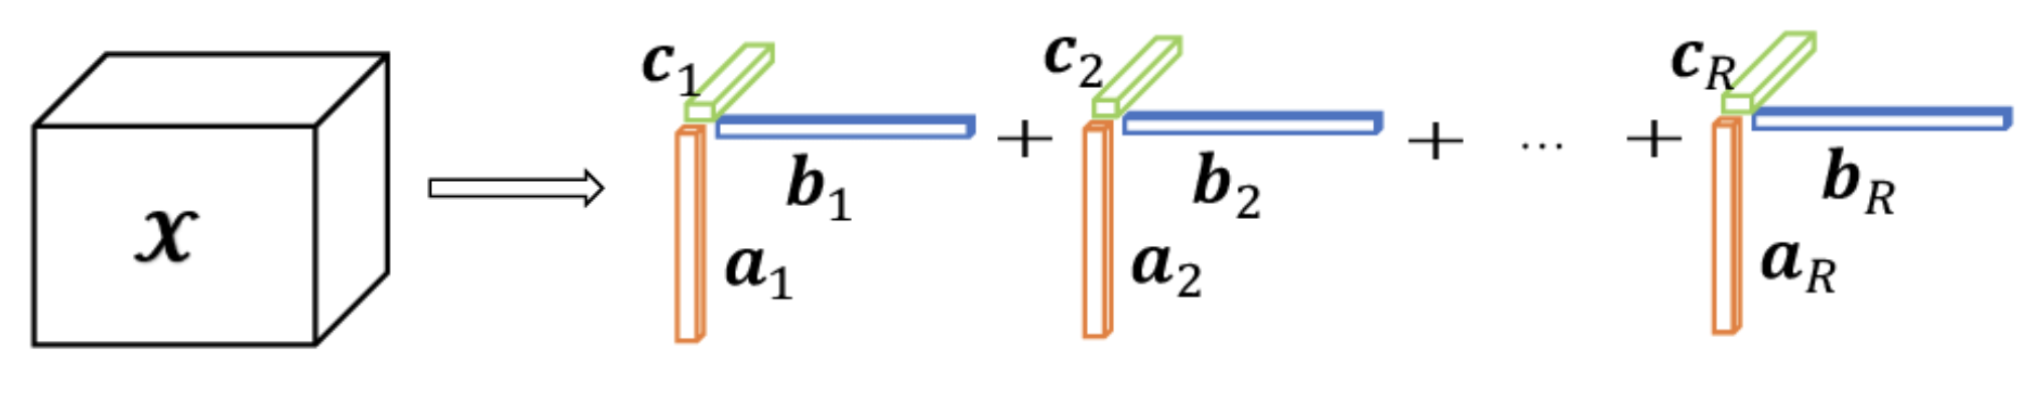
\includegraphics[width=0.95\textwidth]{chapters/varenik2/images/cp-decomposition.png}
\end{figure}
    
Для канонически полиадического разложения задается осевая матризация, для трехмерного случая она имеет вид:
\begin{gather*}
    \vect X_{(1)} \approx \vect A diag(\bm{\lambda})(\vect C\odot \vect B)^T,\\
    \vect X_{(2)} \approx \vect B diag(\bm{\lambda})(\vect C\odot \vect A)^T,\\
    \vect X_{(3)} \approx \vect C diag(\bm{\lambda})(\vect B\odot \vect A)^T.
\end{gather*}
    
Матризация тензора это механизм раскладки тензора в матрицу. Есть осевая матризация, в которой рассматриваются трубки тензора, задаваемые элементами со всеми зафиксированными осями кроме одной - рассматриваемой. Тогда $n$-я осевая матризованная форма $\vect X_{(n)}$ тензора $\vect X \in \mathbb{R}^{I_1\times I_2 \times \dots \times I_N}$ определяется как матрица, в которой столбцы задаются трубками $\vect x_{i_1\dots i_{n-1}\textbf{:}i_{n+1}\dots i_N}$. Еще один тип матризации - на основе срезов (или слайсов), в которой тензор делится на панельки, определяемые элементами со всеми зафиксированными осями, кроме двух. Аналогично осевой матризации, выделенные срезы выстраиваются в матрицу в виде блочных столбцов. В дальнейшем ограничимся только осевой матризацией.

\begin{figure}[h]
	\centering
	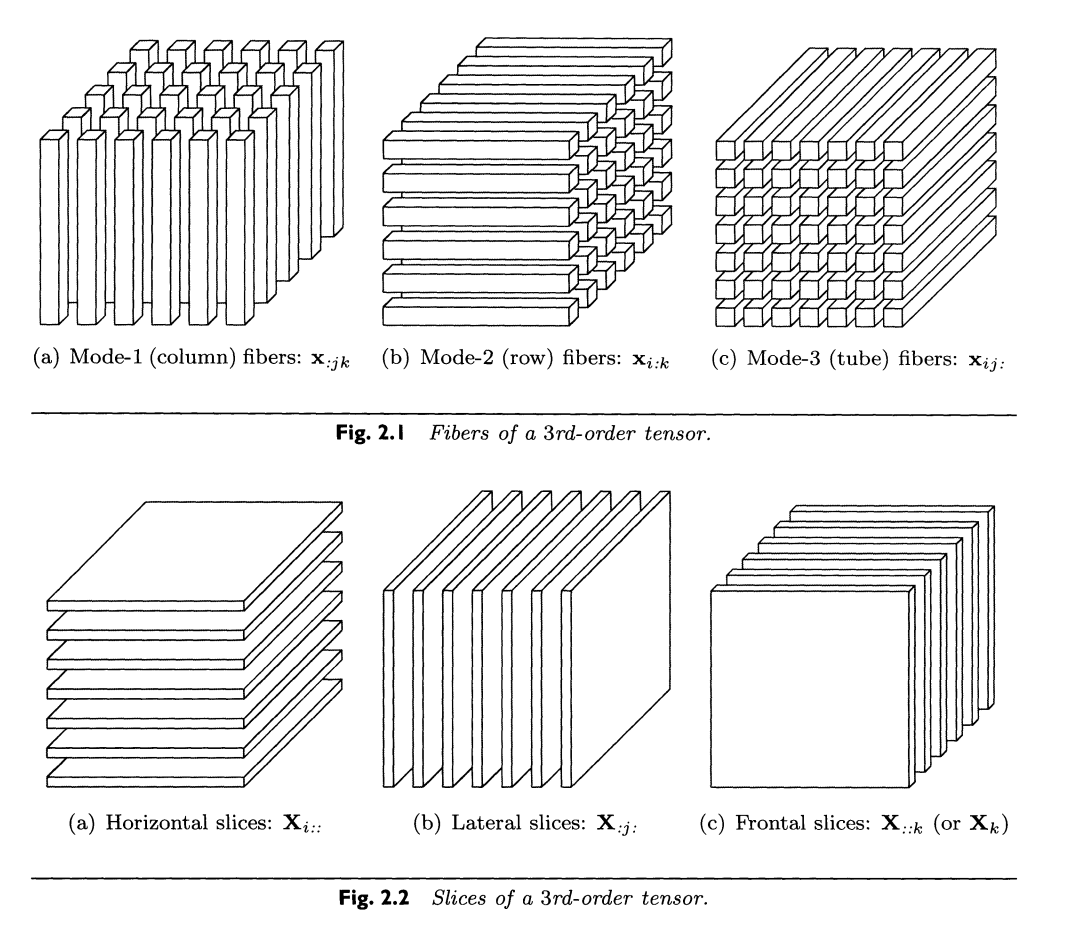
\includegraphics[width=0.7\textwidth]{chapters/varenik2/images/matricization.png}
\end{figure}

\textbf{Свойства}

\begin{itemize}
    \item $rank \vect X$ - наименьшее R необходимое для точной аппроксимации в (\ref{eq1}) при заданном уровне точности разложения;
    \item единственность разложения - при инвариантности к:
        \begin{align*}
            & 1)\text{перестановкам } \vect X = [\bm{\lambda}; \vect A, \vect B, \vect C] = [\bm{\lambda}; \vect A\vect P, \vect B\vect P, \vect C\vect P], \text{ }\vect P \in \mathbb{R}^{R\times R},\\
            & 2)\text{масштабированию } \vect X = \sum_{r=1}^R \lambda_r (\alpha_r \vect a_r) \circ (\beta_r \vect b_r) \circ (\gamma_r \vect c_r), \text{ } \alpha_r\beta_r\gamma_r = 1;
        \end{align*}
    \item вычисляется альтернативным методов наименьших квадратов:
    \begin{align*}
        \min_{\hat{\vect X}} ||\vect X - \hat{\vect X}||_F, \text{где }
        \hat{\vect X} = \sum\limits_{r=1}^R \lambda_r \vect a_r \circ \vect b_r \circ \vect c_r;
    \end{align*}
\end{itemize}

Идея в том, чтобы зафиксировать все фактор-матрицы кроме одной и рассматривать задачу минимизации ошибки аппроксимации относительно незафиксированной матрицы, а затем то же самое повторить для остальных фактор-матриц. Ниже приведет алгоритм вычисления подходящих фактор-матриц и вектора коэффициентов. Он состоит из инициализации и повторения шагов пересчета до тех пор, пока не будет выполнен остановочный критерий. Вектор коэффициентов получается из нормировки фактор-матриц ввиду условия, что их компоненты должны иметь единичную норму.

\begin{figure}[h]
	\centering
	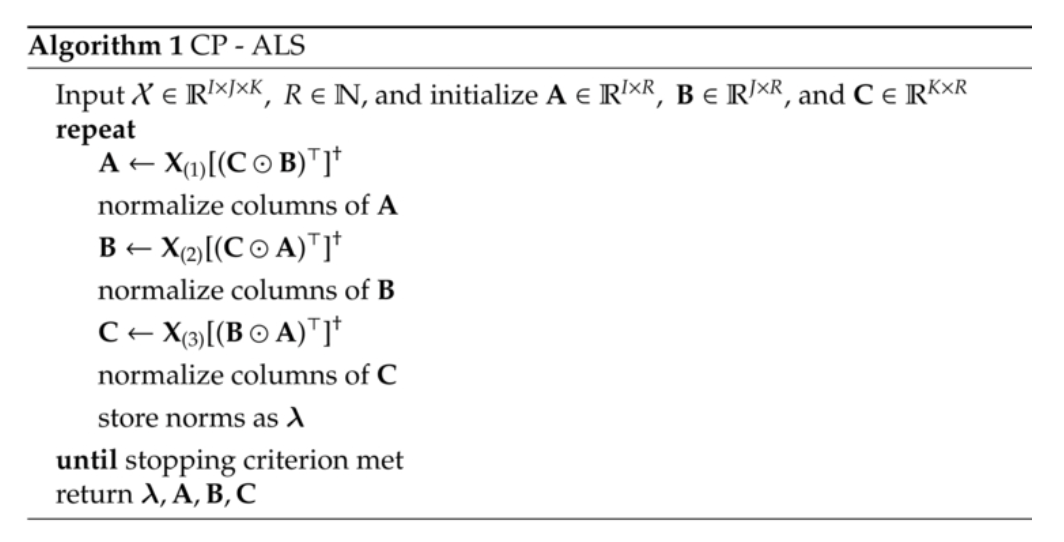
\includegraphics[width=0.8\textwidth]{chapters/varenik2/images/cp-als.png}
\end{figure}

\textbf{N-way}

Пусть $\vect X \in \mathbb{R}^{I_1\times I_2 \times \dots \times I_N}$ - тензор N-го порядка. Тогда канонически полиадическое разложение определяется как:
\begin{gather}
    \vect X \approx \sum\limits_{r=1}^R \lambda_r \vect a_r^{(1)} \circ \vect a_r^{(2)} \circ \dots \circ \vect a_r^{(N)} = [\bm{\lambda}; \vect A^{(1)}, \vect A^{(2)}, \dots, \vect A^{(N)}],
\end{gather}
$$\vect a_r^{(n)} \in \mathbb{R}^{I_n}, ||\vect a_r^{(n)}||_2 = 1, \forall n \in \overline{1, N}.$$
        
При этом осевая матризация:
\begin{gather*}
    \vect X_{(n)} \approx \bm{\Lambda} (\vect A^{(N)} \odot \dots \odot \vect A^{(n+1)} \odot \vect A^{(n-1)} \odot \dots \odot \vect A^{(1)})\vect A^{(n)T}, \text{ } \bm{\Lambda} = diag(\bm{\lambda}).
\end{gather*}

\subsection{Разложение Таккера (Tucker decomposition)}
\textbf{3-way}

Пусть $\vect X \in \mathbb{R}^{I\times J \times K}$ - тензор 3-го порядка. Разложение Таккера предствляет $\vect X$ в виде набора ядра и трех ортогональных фактор-матриц. Такое представление позволяет извлекать информацию о взаимосвязи между различными осевыми компонентами в разложении:
\begin{gather}
    \vect X \approx \vect G \times_1 \vect A \times_2 \vect B \times_3 \vect C = \sum\limits_{r_a=1}^{R_A}\sum\limits_{r_b=1}^{R_B}\sum\limits_{r_c=1}^{R_C} g_{r_a r_b r_c} \vect a_{r_a} \circ \vect b_{r_b} \circ \vect c_{r_c} = [\vect G; \vect A, \vect B, \vect C],
    \label{eq2}
\end{gather}
$\vect A \in \mathbb{R}^{I\times R_A}, \vect B \in \mathbb{R}^{J\times R_B}, \vect C \in \mathbb{R}^{K\times R_C} - \text{фактор-матрицы}$, которые могут рассматриваться как главные компоненты каждой оси, 
$\vect G\in \mathbb{R}^{R_A\times R_B \times R_C}$ - ядро, отображающее уровень взаимодействия между разными компонентами.

\begin{figure}
	\centering
	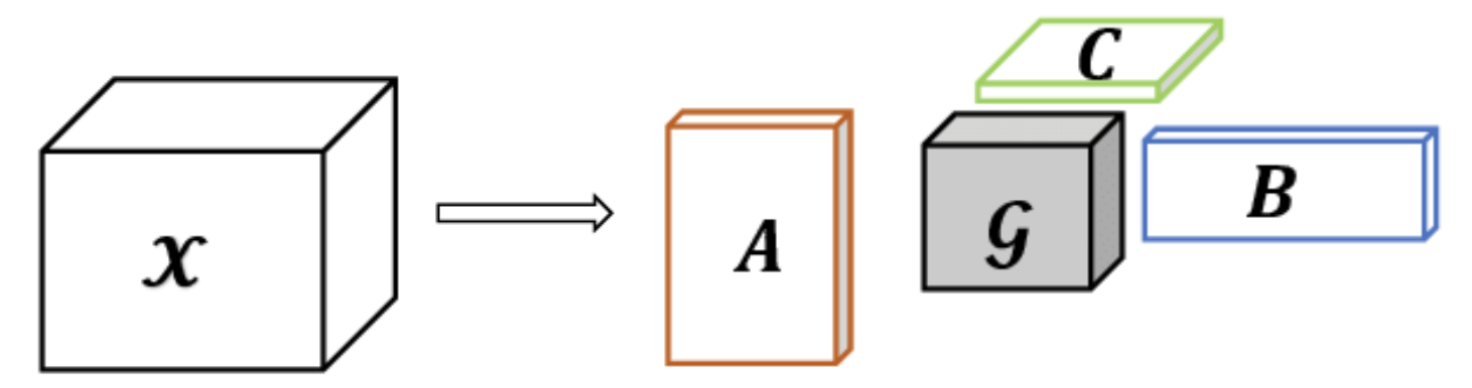
\includegraphics[width=0.72\textwidth]{chapters/varenik2/images/tucker-decomposition.png}
\end{figure}

Матризованная форма:
\begin{gather*}
    \vect X_{(1)} \approx \vect A \vect G_{(1)}(\vect C\otimes \vect B)^T,\\
    \vect X_{(2)} \approx \vect B \vect G_{(2)}(\vect C\otimes \vect A)^T,\\
    \vect X_{(3)} \approx \vect C \vect G_{(3)}(\vect B\otimes \vect A)^T.
\end{gather*}
  
\textbf{Свойства}

\begin{itemize}
    \item частичный ранг $rank_n \vect X$ - количество столбцов матрицы $\vect X_{(n)}$;
    \item при $\vect B = \vect I, \vect C = \vect I$ соответствует стандартному двумерному PCA: $\vect X_{(1)} = \vect A \vect G_{(1)}$;
    \item вычисляется методом HOSVD:
    \begin{align*}
        \min_{\vect G, \vect A, \vect B, \vect C} ||\vect X - [\vect G; \vect A, \vect B, \vect C]_{\text{Tucker}}||_F;
    \end{align*}
\end{itemize}

\begin{figure}[h]
	\centering
	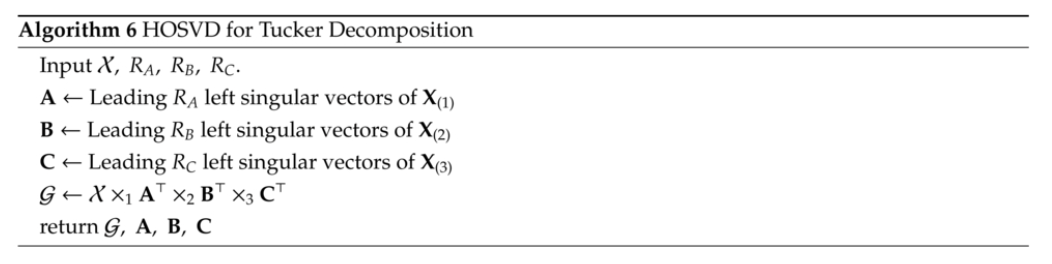
\includegraphics[width=0.95\textwidth]{chapters/varenik2/images/hosvd.png}
\end{figure}
    
\textbf{N-way}

Аналогично определяется $N$-мерное расширение разложения Таккера, которое представляет собой матричное произведение ядра на $N$ фактор матрицы.

Пусть $\vect X \in \mathbb{R}^{I_1\times I_2 \times \dots \times I_N}$, тогда:
\begin{gather*}
    \vect X = \vect G \times_1 \vect A^{(1)} \times_2 \vect A^{(2)} \times_3 \dots \times_N \vect A^{(N)} = [\vect G; \vect A^{(1)}, \vect A^{(2)}, \dots, \vect A^{(N)}],\\
    \vect X_{(n)} = \vect A^{(n)} \vect G_{(n)} (\vect A^{(N)} \otimes \dots \otimes \vect A^{(n+1)} \otimes \vect A^{(n-1)}\otimes \dots \otimes \vect A^{(1)})^T.
\end{gather*}


Таким образом, CP обладает свойством уникальности при достаточно слабых условиях, но при этом пренебрегает взаимодействием между компонентами в разных осях.
Разложение Таккера в общем случае неединственно, что затрудняет интерпретацию полученной скрытой структуры данных, но при этом является обобщением CP разложения для возможности учета информации о взаимных связях.
    
\subsection{Обобщение PLS на тензорный случай: N-way PLS и HOPLS}

\textbf{Standard PLS}

В системах BCI, в задачах регрессии линейные модели применяются в основном из-за их простоты и надежности, при этом высокая размерность данных затрудняет прямое применение общих методов линейной регрессии. Регрессия методом частичных наименьших квадратов как раз подходит для таких ситуаций.

Решая задачу методом частничных наименьших квадратов проблема сводится к нахождению общего скрытого пространства, одновременно хорошо аппроксимирующего $X$ и $Y$.

Метод PLS раскладывает исходную матрицу на произведение матрицы представления в скрытом пространстве и матрицы перехода, что можно также записать в виде суммы матриц единичного ранга.

\begin{gather*}
    \vect X = \vect T \vect P^T + \vect E = \sum_{r=1}^R \vect t_r \vect p_r^T + \vect E, \text{ }\vect X \in \mathbb{R}^{I\times J} - \text{матрица объектов}\\
    \vect Y = \vect U \vect Q^T + \vect F = \sum_{r=1}^R \vect u_r \vect q_r^T + \vect F, \text{ }\vect Y \in \mathbb{R}^{I\times M} - \text{матрица ответов},
\end{gather*}
$\vect T, \vect U \in \mathbb{R}^{I\times R}$ - матрицы описания $\vect X$ и $\vect Y$ в скрытом пространстве,\\ 
$\vect P \in \mathbb{R}^{J\times R}, \vect Q \in \mathbb{R}^{M\times R}$ - матрицы перехода в скрытое пространство, \\
$\vect E \in \mathbb{R}^{I\times J}, \vect F \in \mathbb{R}^{I\times M}$ - матрицы невязок.

В предположении наличия линейной связи $\vect u \approx d\vect t$, получаем задачу нахождения совместной матрицы Т, наилучшим образом описывающей исходные $X$ и $Y$:
\begin{gather*}
    \vect Y = \vect T \vect D \vect Q^T + \vect F = \sum_{r=1}^R d_{rr}\vect t_r \vect q_r^T + \vect F, \text{ } \vect D = diag(d_{rr}), \text{ } d_{rr} = \frac{\vect u_r^T \vect t_r}{\vect t_r^T \vect t_r}
\end{gather*}

\begin{figure}[h]
	\centering
	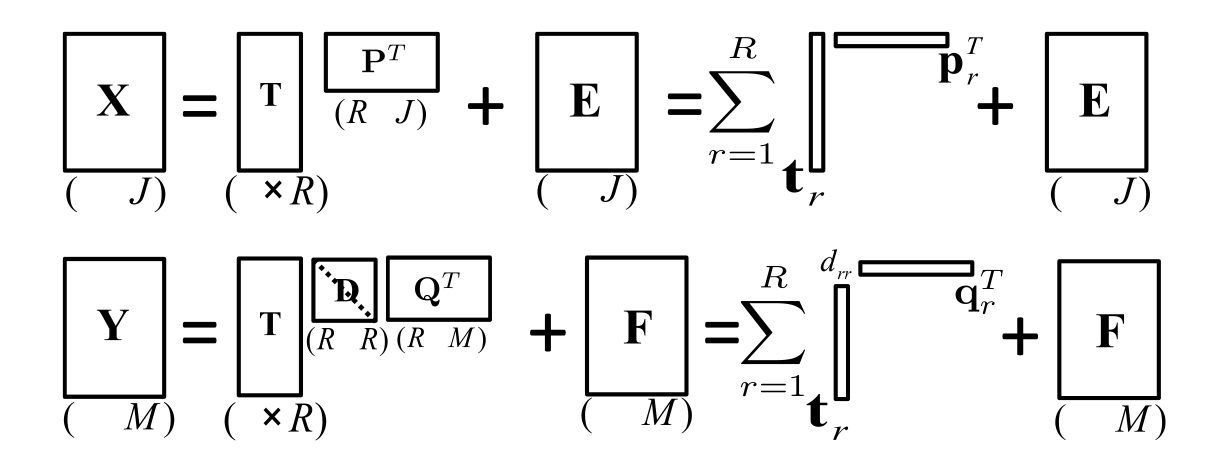
\includegraphics[width=0.7\textwidth]{chapters/varenik2/images/pls.png}
\end{figure}

\newpage
\textbf{N-way PLS}

Для тензорного случая имеется простое прямое обобщение PLS. А именно, пусть имеется тензор объектов 4 порядка $\vect X \in \mathbb{R}^{I\times L\times K\times J}$, и матрица ответов $\vect Y \in \mathbb{R}^{I\times N}$. Тогда с использованием CP разложения NPLS принимает вид, в котором $X$ представляется в виде суммы внешних произведений скрытого вектора на векторы перехода, соответствующие отдельным признаковым доменам. Поскольку Y -  матрица, ее разложение определяется стандартным образом:
\begin{gather*}
    \vect X = \sum\limits_{r=1}^R \vect t_r \circ \vect p_r \circ \vect q_r \circ \vect s_r + \vect E,\\
    \vect Y = \sum\limits_{r=1}^R d_{rr}\vect t_r \vect c_r^T + \vect F, \text{где}
\end{gather*}
$\vect t_r \in \mathbb{R}^{I\times 1}$ - скрытый вектор, $\vect p_r \in \mathbb{R}^{L\times 1}, \vect q_r \in \mathbb{R}^{K\times 1}, \vect s_r \in \mathbb{R}^{J\times 1}$ - векторы перехода.\\~\

При NPLS оговаривается, что $\forall r = 1, \dots R$ векторы $\vect p, \vect q, \vect s, \vect c$ определяются из условия максимизации ковариации между скрытыми представлениями:
\begin{gather*}
    [\vect p, \vect q, \vect s, \vect c] = \arg \max_{\vect p, \vect q, \vect s, \vect c} [cov(\vect t, \vect u)], \text{ при}\\
    t_i = \sum\limits_{l=1}^L\sum\limits_{k=1}^K\sum\limits_{j=1}^J x_{ilkj}p_l q_k s_j = \vect y_i \vect c, \text { и }
    ||\vect p||_2^2 = ||\vect q||_2^2 = ||\vect s||_2^2 = 1
\end{gather*}

\textbf{HOPLS}

Рассмотрим еще одно обобщение PLS, называемое HOPLS. В нем используется разложение Таккера для отображения более сложных зависимостей. Его использование обосновывается фактом, что разложение Таккера является ранговой подпространственной аппроксимацией в отличии от CP, которое является простой аппроксимацией низшего ранга. Исходя из этого в работе предполагается, что модель на основе разложения Таккера лучше справляется с аппроксимацией данных.

\begin{figure}
	\centering
	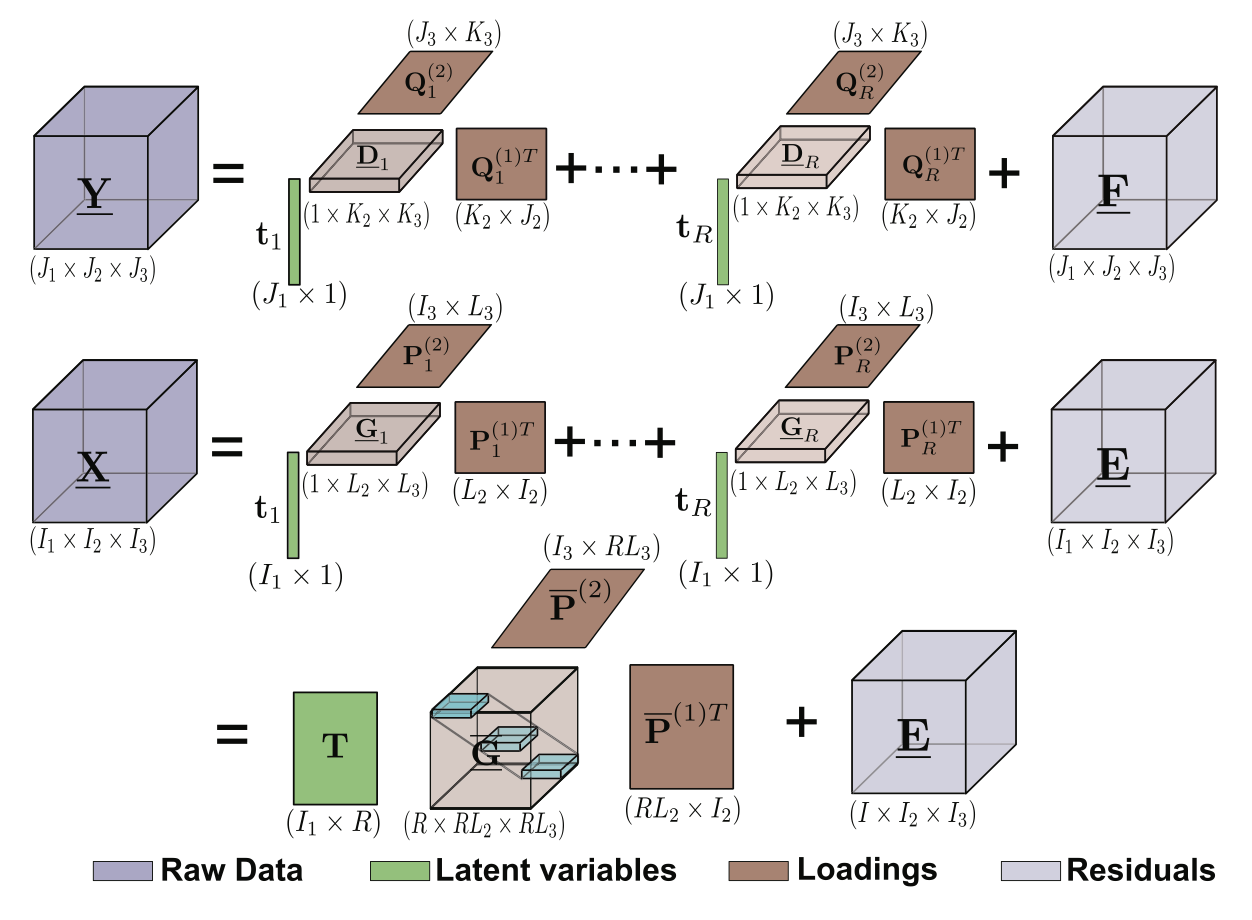
\includegraphics[scale=0.55]{chapters/varenik2/images/hopls.png}
\end{figure}
 
Заметим, что используется не стандартное разложение Таккера, а его комбинации с CP разложением. В итоге, исходный тензор представляется в виде суммы блоков Таккера, которые потом объединяются в общее представление с блочнодиагоальным ядром.

Пусть $\vect X \in \mathbb{R}^{I_1\times \dots \times I_N}, \vect Y \in \mathbb{R}^{J_1\times \dots \times J_M}$, при этом $I_1 = J_1$. Модель HOPLS определяется как: 
\begin{gather*}
    \vect X = \vect G \times_1 \vect T \times_2 \vect P^{(1)} \times_3 \dots \times_N \vect P^{(N-1)} + \vect E,\\
    \vect Y = \vect D \times_1 \vect T \times_2 \vect Q^{(1)} \times_3 \dots \times_M \vect Q^{(M-1)} + \vect F, 
\end{gather*}
где ядро-тензоры
\begin{gather*}
    \vect G = blockdiag(\vect G_1, \dots, \vect G_R) \in \mathbb{R}^{R\times RL_2 \times \dots \times RL_N},\\
    \vect D = blockdiag(\vect D_1, \dots, \vect D_R) \in \mathbb{R}^{R\times RK_2 \times \dots \times RK_M},
\end{gather*}
$\vect T\in \mathbb{R}^{I_1\times R}$ - матрица скрытых переменных,\\
$\vect P^{(n)} = [\vect P_1^{(n)}, \dots, \vect P_R^{(n)}]$, $\vect Q^{(m)} = [\vect Q_1^{(m)}, \dots, \vect Q_R^{(m)}]$ - матрицы перехода для оси $n$ и $m$ соответственно.

\textbf{Применение}

Что касается применения к декодированию, в работе HOPLS проводилось исследование по сравнению стандартного PLS, NPLS и HOPLS в задаче прогнозирования движения руки в 3-мерном пространстве по 4 маркерам установленным на руке, запястье, локте и плече. В качестве данных использовались электрокортикограммы, которые рассматривались в 4 доменах: эпоха, время, частота, пространство. Были получены результаты в которых HOPLS значимо превосходит своих предшественников, при этом исходя из посчитанной точности видно, что NPLS не гарантирует лучшей производительности по сравнению со стандартным матричным подходом.

\begin{figure}[h]
    \centering
    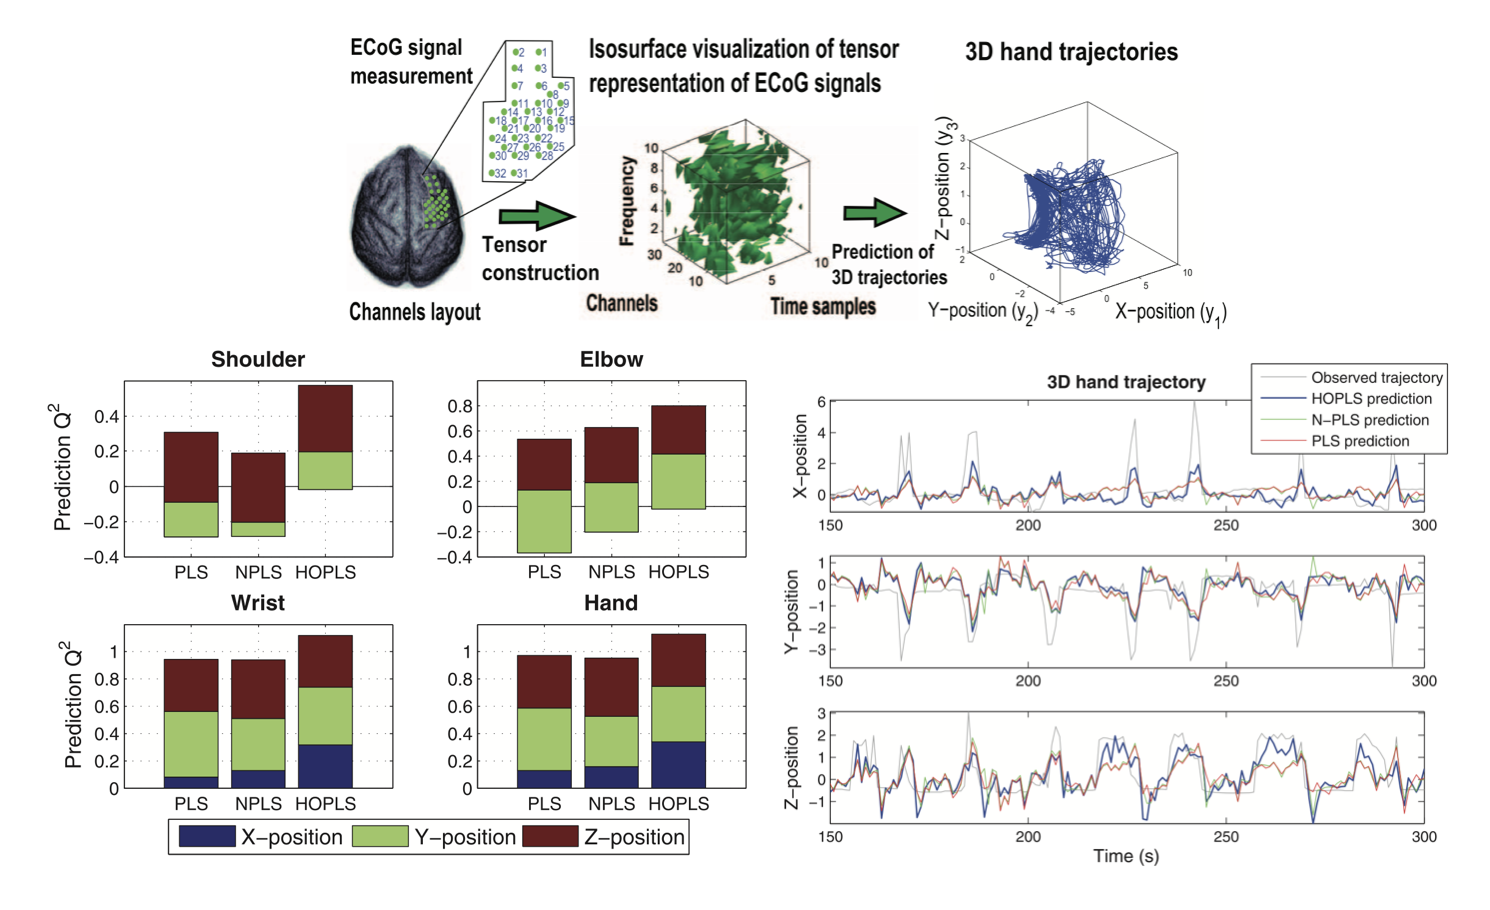
\includegraphics[scale=0.65]{chapters/varenik2/images/result.png}
\end{figure}

\section{Questions To Discussion}
\begin{enumerate}
    \item Чем отличаются конструкции CP и Tucker разложения?
    \item При каком условии одно разложения является частным другого?
    \item Какой общий принцип используется для вычисления разложений?
    \item В чем состоит подход альтернативного метода наименьших квадратов для CP разложения?
    \item Чем объясняется очевидность обобщения стандартного PLS до NPLS?
\end{enumerate}
    
    \clearpage
    \chapter{Fourier Neural Operator for Parametric Partial Differential Equations}
    \section{Введение}

Многие задачи в науке и технике включают многократное решение сложных систем дифференциальных уравнений в частных производных (PDE) для различных значений параметров. Примеры возникают в молекулярной динамике, микромеханике и турбулентных потоках. В данной главе рассмотрен метод 

\section{Литература}

	\begin{itemize}
		\item ~\cite{FNO} --  работа, в которой описан подход нейронного Фурье оператора для  дифференциальных уравнений в частных производных
		\item ~\cite{Deeponet} -- работа, в которой описан подход нейронного оператора. На основе данной статьи построен метод нейронного Фурье оператора
		\item ~\cite{FNOcode} -- код с реализацией метода нейронного Фурье оператора 
	\end{itemize}


\section{Нейронный Фурье оператор для дифференциальных уравнений в частных производных}

Традиционные методы, такие как методы конечных элементов (FEM) и методы конечных разностей (FDM), решают уравнения путем дискретизации пространства. Грубые сетки работают быстро, но менее точно; подробные сетки точны, но медленны. Сложные системы PDE обычно требуют очень точной дискретизации, поэтому сложны в обработке и отнимают много времени для традиционных методов решения. Кроме того, решение сильно зависит от разрешения сетки.


\subsection{Обзор существующих решений}
	\begin{itemize}
		\item \textbf{Традиционные методы (методы конечных элементов (FEM) и методы конечных разностей (FDM))}: медленно, вычислительно затратно
		\item \textbf{Конечномерные операторы}. Эти подходы параметризуют оператор-решение как глубокую сверточную нейронную сеть между конечномерными евклидовыми пространствами. Зависят от разрешения сетки и ограничены геометрией обучающих данных.
		\item \textbf{Neural-FEM}: параметризует функцию-решение  нейронной сетью. Этот подход моделирует один экземпляр уравнений с конкретными параметрами, а не оператор-решение. Он не зависит от сетки и точен, но для любого нового функционального параметра/коэффициента он требует обучения новой нейронной сети. Вычислительно затратный.
		\item \textbf{Нейронные операторы}: не зависит от сетки, моделирует бесконечномерные операторы. Нейронная сеть может быть использована для различных дискретизаций. Но вычислительно затратно получение интегральных операторов, на основе которых построено решение.
		\item \textbf{Нейронные Фурье операторы}: не зависит от сетки, моделирует бесконечномерные операторы, интегральный оператор принимается сверткой и создается посредством линейного преобразования в Фурье области. Подобно тому, как стандартные нейронные сети аппроксимируют сильно нелинейные функции, комбинируя линейное умножение с нелинейными активациями, предлагаемые нейронные операторы могут аппроксимировать сильно нелинейные операторы.
	\end{itemize}

\subsection{Постановка задачи}
	\begin{itemize}
		\item Пусть $D \subset \mathbb{R}^{a}$ -- ограниченное, открытое множество, $\mathcal{A}=\mathcal{A}\left(D ; \mathbb{R}^{d_{a}}\right)$ и $\mathcal{U}=\mathcal{U}\left(D ; \mathbb{R}^{d_{u}}\right)$ -- сепарабельные банаховы пространства функций
		\item Пусть $G^{\dagger}: \mathcal{A} \rightarrow \mathcal{U}$ -- нелинейное отображение, оператор решения параметрического уравнения в частных производных
		\item Пусть имеем наблюдения $\left\{a_{j}, u_{j}\right\}_{j=1}^{N}$, где $a_{j} \sim \mu$ -- i.i.d. последовательность из вероятностной меры $\mu$ на $\mathcal{A}$, $u_{j}=G^{\dagger}\left(a_{j}\right)$ 
		\item Требуется построить аппроксимацию $G^{\dagger}$
		$$
		G_{\theta}: \mathcal{A} \rightarrow \mathcal{U}, \quad \theta \in \Theta, \quad \quad \quad G_{\theta^{\dagger}} \approx G^{\dagger}, \quad \theta^{\dagger} \in \Theta
		,$$
		где $\Theta$ -- конечномерное пространство параметров
		\item Задача оптимизации
		$$
		\min_{\theta \in \Theta} \mathbb{E}_{a \sim \mu}\left[C\left(G_{\theta}(a), G^{\dagger}(a)\right)\right]
		,$$
		где $C: \mathcal{U} \times \mathcal{U} \rightarrow \mathbb{R}$ -- функция ошибки
	\end{itemize}

Аппроксимация оператора $G^{\dagger}$ -- это другая и обычно гораздо более сложная задача, чем поиск решения $u \in \mathcal{U}$ уравнения в частных производных для одного экземпляра параметра $a \in \mathcal{A} .$. Подход с нейронным Фурье оператором напрямую аппроксимирует оператор и, следовательно, работает быстрее и предлагает огромную экономию вычислений по сравнению с традиционными методами решений.

\subsection{Нейронный оператор}
Нейронный оператор имеет итеративную структуру решения:
$$a\mapsto v_{0} \mapsto v_{1} \mapsto \ldots \mapsto v_{T} \mapsto u,$$
где $v_{j}, j=0,1, \ldots, T-1$ -последовательность функций, $v_{0}(x)=P(a(x))$,  $u(x)=Q\left(v_{T}(x)\right), Q: \mathbb{R}^{d_{v}} \rightarrow \mathbb{R}^{d_{u}}$. Сначала вход $a$ переводится в до представления более высокой размерности с помощью преобразования $P(.)$, которое обычно параметризуется неглубокой полносвязной нейронной сетью. Далее применяются несколько раз слои нейронного оператора. В конце получаем проекцию $v_T$ преобразованием $Q(.)$, которое тоже параметризуется полносвязным слоем.

\textbf{Определение 1 (Слой нейронного оператора)}
	$$v_{t+1}(x):=\sigma\left(W v_{t}(x)+\left(\mathcal{K}(a ; \phi) v_{t}\right)(x)\right), \quad \forall x \in D,$$
	где  $\mathcal{K}(a ; \phi)$ -- ядерный интегральный оператор, $W: \mathbb{R}^{d_{v}} \rightarrow \mathbb{R}^{d_{v}}$ -- линейное преобразование, $\sigma: \mathbb{R} \rightarrow \mathbb{R}$ -- нелинейная функция активации


\textbf{Определение 2 (Ядерный интегральный оператор)}
	$$
	\left(\mathcal{K}(a ; \phi) v_{t}\right)(x):=\int_{D} \kappa(x, y, a(x), a(y) ; \phi) v_{t}(y) \mathrm{d} y, \quad \forall x \in D,$$
	где  $\kappa_{\phi}: \mathbb{R}^{2\left(d+d_{a}\right)} \rightarrow \mathbb{R}^{d_{v} \times d_{v}}$ --  нейросеть, параметризованная $\phi \in \Theta_{\mathcal{K}}$

\subsection{Нейронный оператор Фурье}
Обозначим через $\mathcal{F}$ преобразование Фурье функции $f: D \to R^{d_v}$, а через $\mathcal{F}^{-1}$ -- обратное.
\begin{itemize}
	\item Если убрать зависимость от функции $a$ и принять $\kappa_{\phi}(x, y)=\kappa_{\phi}(x-y)$, то получим, что $\left(\mathcal{K}(a ; \phi) v_{t}\right)(x)$ -- оператор свертки
	\item Применяя теорему о свертке, получаем:
	$$
	\left(\mathcal{K}(a ; \phi) v_{t}\right)(x)=\mathcal{F}^{-1}\left(\mathcal{F}\left(\kappa_{\phi}\right) \cdot \mathcal{F}\left(v_{t}\right)\right)(x) $$
	
\end{itemize}

\textbf{Определение 3 (Интегральный оператор Фурье)}
	$$
	\left(\mathcal{K}(\phi) v_{t}\right)(x)=\mathcal{F}^{-1}\left(R_{\phi} \cdot\left(\mathcal{F} v_{t}\right)\right)(x) \quad \forall x \in D,
	$$ 
	где $R_{\phi}$ -- преобразование Фурье функции $\kappa: \bar{D} \rightarrow \mathbb{R}^{d_{v} \times d_{v}}$ параметризованной $\phi \in \Theta_{\mathcal{K}}$
	
\subsection{Структура нейронной сети}
	Реализация нейронного Фурье оператора состоит из последовательного применения четырех интегральных Фурье операторов с активацией ReLU, а также с батч-нормализацией. 
	\begin{figure}[h]
		\centering
		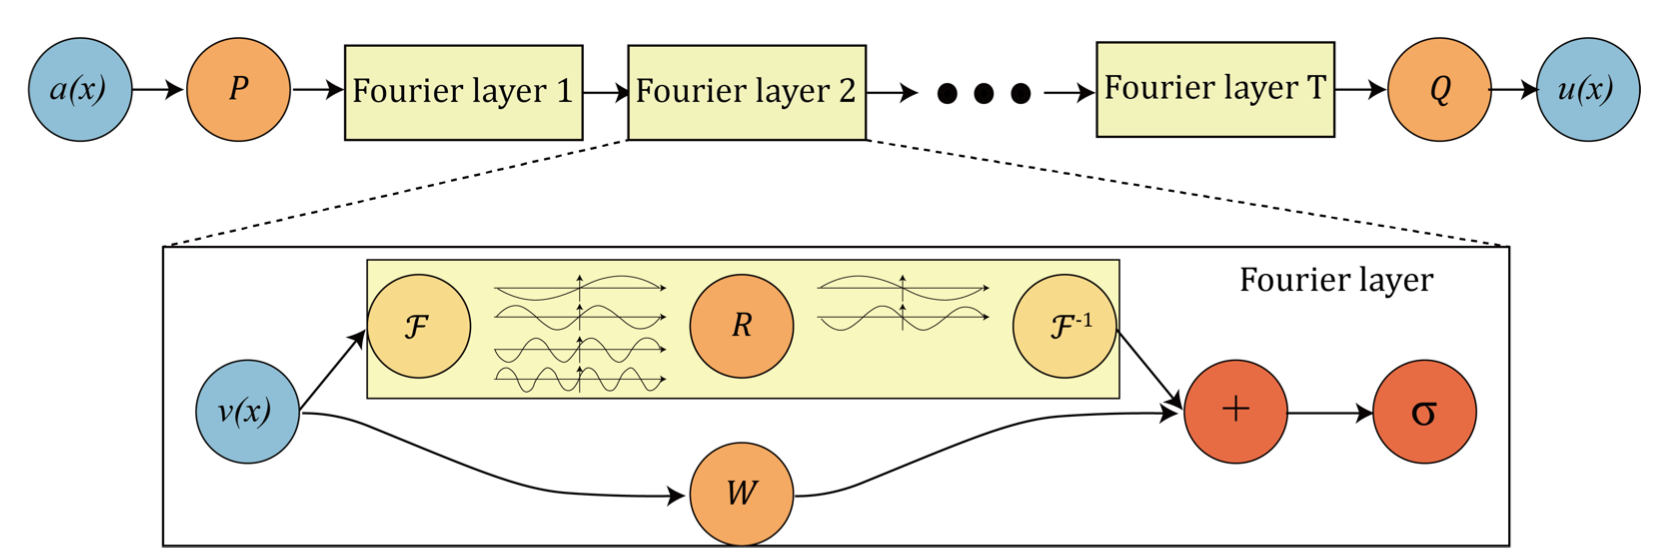
\includegraphics[width=0.99\textwidth]{architecture.png}
		\caption{Рис.  Структура нейронных Фурье операторов}
	\end{figure}

\subsection{Вычислительный эксперимент}
В работе Fourier Neural Operator for Parametric Partial Differential Equations были приведены эксперименты с нейронным Фурье оператором. Авторы работы сравнили предложенный ими нейронный Фурье оператор с несколькими конечномерными архитектурами на примере одномерного уравнения Бюргерса, двумерной задачи потока Дарси и двумерного уравнения Навье-Стокса.

Результаты представлены на рисунке 2.
\begin{figure}[h]
	\centering
	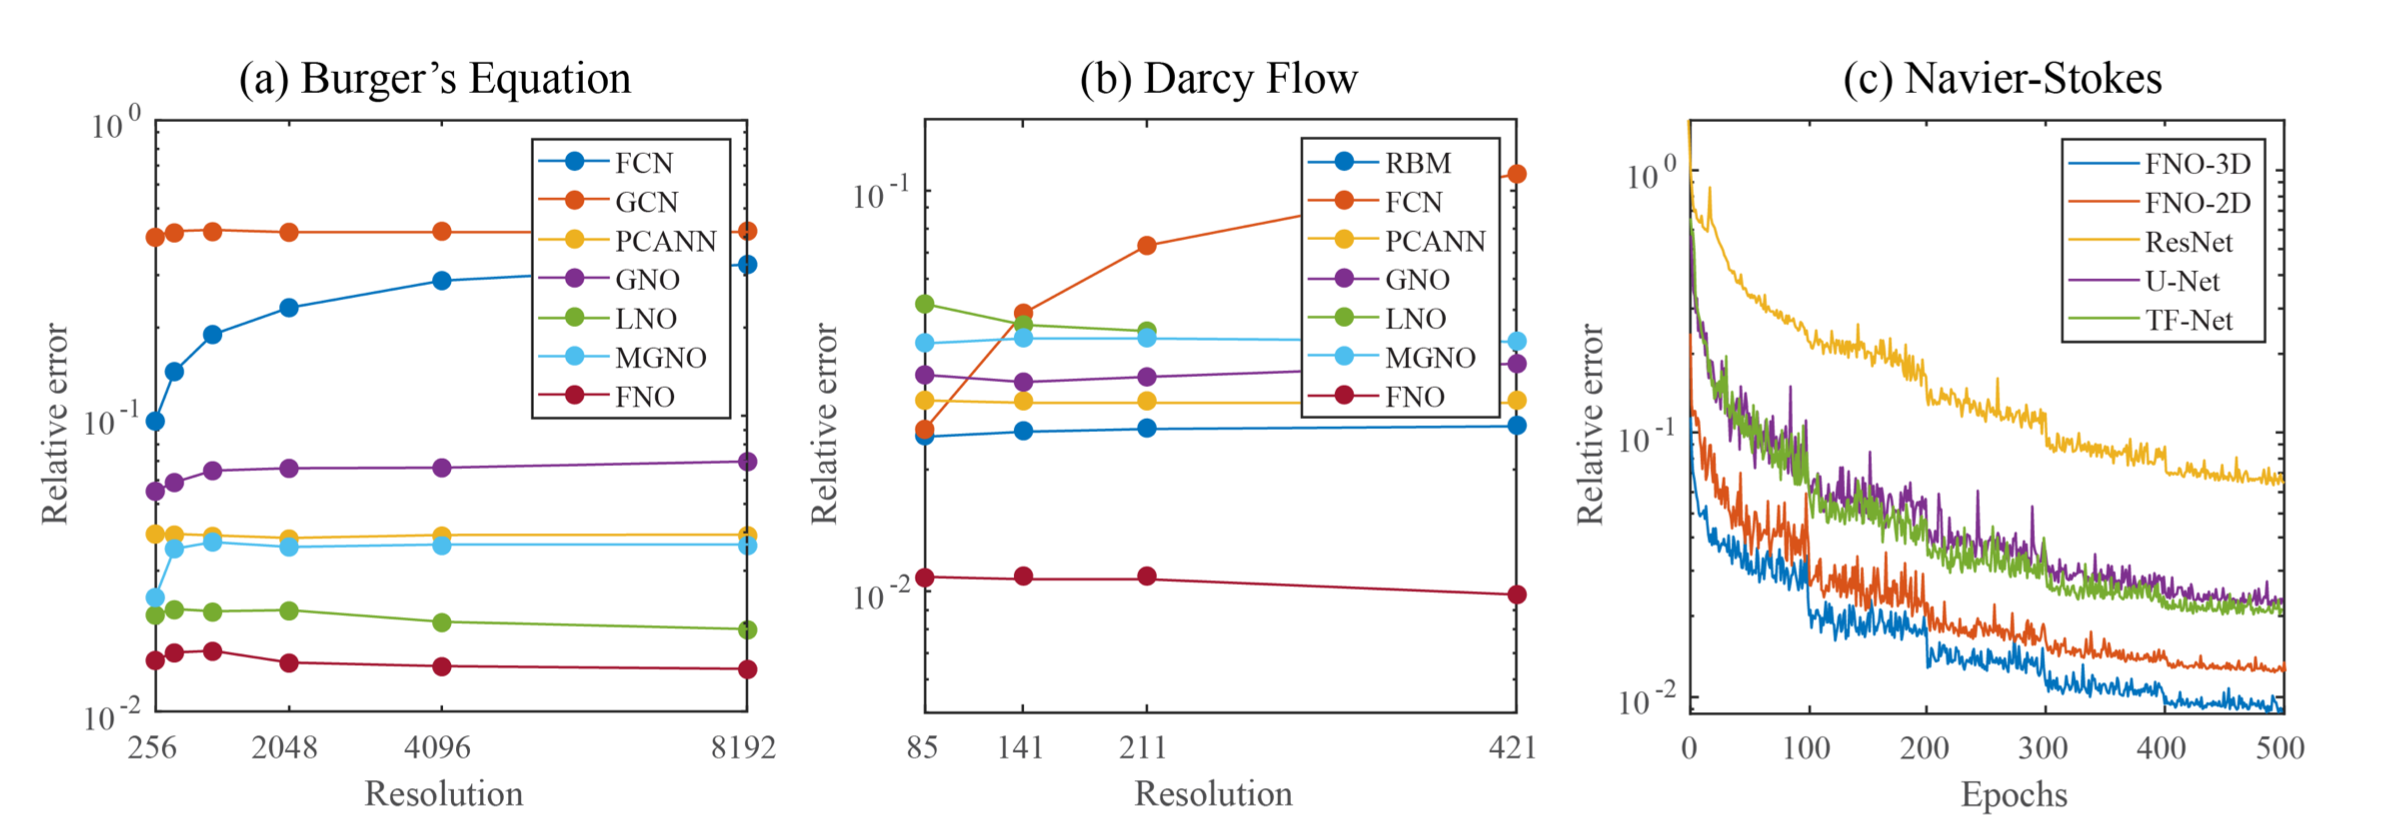
\includegraphics[width=0.99\textwidth]{experiments.png}
	\caption{Рис. Результаты экспериментов для уравнения Бюргерса, потоков Дарси, уравнениий Навье — Стокса}
\end{figure}

\begin{enumerate}
	\item \textbf{FNO}: the newly purposed Fourier neural operator.
	\item \textbf{FNO-2d}: 2-d Fourier neural operator with a RNN structure in time.
	\item \textbf{FNO-3d}: 3-d Fourier neural operator that directly convolves in space-time.
	\item NN: a simple point-wise feedforward neural network.
	\item RBM: the classical Reduced Basis Method (using a POD basis) 
	\item FCN: a the-state-of-the-art neural network architecture based on Fully Convolution Networks
	\item PCANN: an operator method using PCA as an autoencoder on both the input and output data and interpolating the latent spaces with a neural network
	\item GNO: the original graph neural operator
	\item MGNO: the multipole graph neural operator
	\item LNO: a neural operator method based on the low-rank decomposition of the kernel $\kappa(x, y):=\sum_{j=1}^{r} \phi_{j}(x) \psi_{j}(y)$ similar to the unstacked DeepONet
	\item ResNet: 18 layers of 2-d convolution with residual connections
	\item U-Net: A popular choice for image-to-image regression tasks consisting of four blocks with 2-d convolutions and deconvolutions
	\item TF-Net: A network designed for learning turbulent flows based on a combination of spatial and temporal convolutions 
	
\end{enumerate}


\subsection{Уравнения Навье-Стокса}
В работе также была приведена визуализация решения уравнений Навье-Стокса (Рис. 3)
$$
\begin{aligned}
\partial_{t} w(x, t)+u(x, t) \cdot \nabla w(x, t) &=\nu \Delta w(x, t)+f(x), & & x \in(0,1)^{2}, t \in(0, T] \\
\nabla \cdot u(x, t) &=0, & & x \in(0,1)^{2}, t \in[0, T] \\
w(x, 0) &=w_{0}(x), & & x \in(0,1)^{2}
\end{aligned}
$$

\begin{figure}[h]
	\centering
	%\includegraphics[width=1.02\textwidth]{experiment.pdf}
	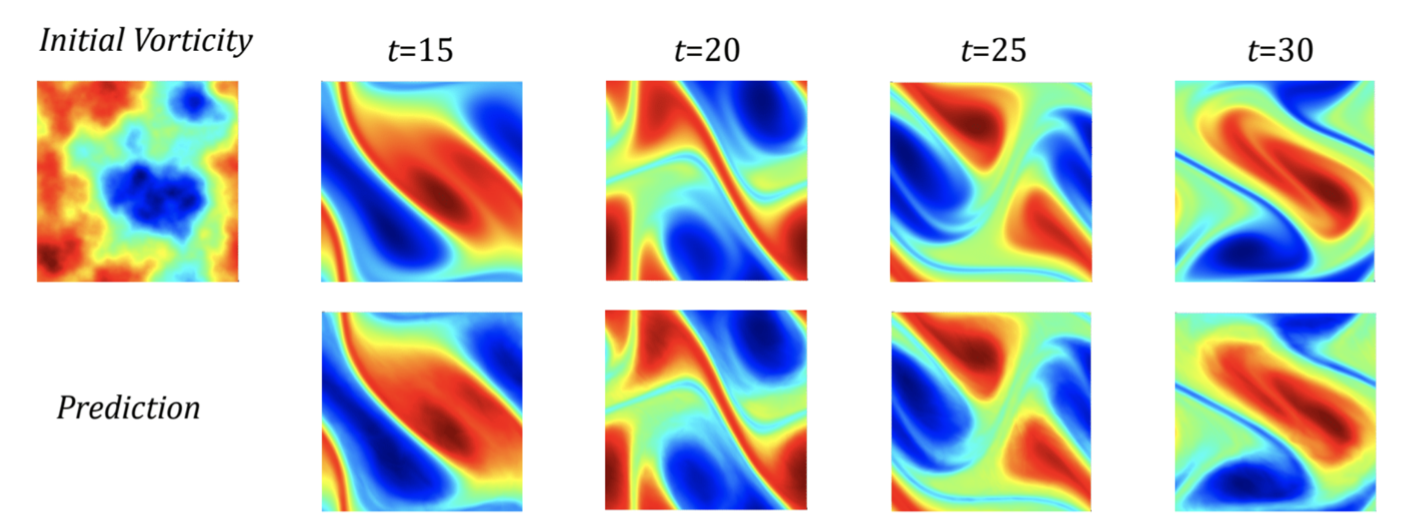
\includegraphics[width=0.99\textwidth]{navier_example.png}
	\caption{Рис. Пример потока из Навье-Стокса: истинные потоки сверху, предсказания нейронного Фурье оператора снизу}
	\label{fig:experiment}
\end{figure}

	
\section{Вопросы на обсуждение}

	\begin{itemize}
	\item Какие недостатки у традиционных методов решения по сравнения с нейронными Фурье  операторами?
	\item Как преобразование Фурье решает проблемы нейронного оператора? 
	\item Какие матрицы обучаются в слое нейронного Фурье оператора?
	\item Какая идея лежит в добавлении слагаемого $Wv_t(x)$ в слое нейронного оператора? 
\end{itemize}
    
    \clearpage
    \chapter{Hamiltonian and Lagrangian Neural Networks}
    \section{Введение}

В данной главе рассматривается проблема моделирования физических систем, решение дифференциальных уравнений с применением нейронных сетей. В этой области имеется проблема: существующие подходы с нейронными сетями не имеют априорных знаний о физике. Это мешает им выучить точные физические законы. В главе рассмотрен один из подходов, как решать эту проблему: учить из данных законы сохранения/инвариантные величины на основе гамильтоновой или лагранжевой механики.

\section{Литература}

\begin{itemize}
	\item \textit{Greydanus et al.} Hamiltonian Neural Networks, // Advances in Neural Information Processing Systems, 2019
	\item \textit{M. Cranmer, Greydanus et al.} Lagrangian Neural Networks // arXiv preprint, 2020
	\item \textit{Greydanus et al.}  Blog post on Hamiltonian Neural Networks // \\https://greydanus.github.io/2019/05/15/hamiltonian-nns
	\item \textit{Greydanus et al.}  Blog post on Lagrangian Neural Networks article // \\https://greydanus.github.io/2020/03/10/lagrangian-nns
\end{itemize}


\section{Hamiltonian and Lagrangian Neural Networks}

Вспомним, как решается рассматриваемая задача в классических подходах теоретической механики. Рассмотрим подход с гамильтоновй механикой.

\subsection{Гамильтонова механика}
\begin{enumerate}
	\item Выбрать набор координат, описывающих состояние системы: $\textbf{q}=(q_1, \cdots,q_N)$ -- позиции, $\textbf{p}=(p_1,\cdots,p_N)$ -- импульсы.
	\item Записать полную энергию системы как функцию этих координат (гамильтониан $\mathcal{H}$). 
	\item Используя уравнения Гамильтона, найти производные системы по времени:
	$$
	\frac{d \mathbf{q}}{d t}=\frac{\partial \mathcal{H}}{\partial \mathbf{p}}, \quad \frac{d \mathbf{p}}{d t}=-\frac{\partial \mathcal{H}}{\partial \mathbf{q}}
	$$
	Получили эволюцию координат ($\textbf{q, p}$) по времени: $
	\mathbf{S}_{\mathcal{H}}=\left(\frac{\partial \mathcal{H}}{\partial \mathbf{p}},-\frac{\partial \mathcal{H}}{\partial \mathbf{q}}\right)
	$
	\item Интегрировать полученные производные по времени для получения состояния системы в какой-то момент времени в будущем: $$ \left(\mathbf{q}_{1}, \mathbf{p}_{1}\right)=\left(\mathbf{q}_{0}, \mathbf{p}_{0}\right)+\int_{t_{0}}^{t_{1}} \mathbf{S}(\mathbf{q}, \mathbf{p}) d t$$
	
\end{enumerate}

На основе этой последовательности действий строится Гамильтонова нейронная сеть:


\subsection{Hamiltonian Neural Networks}

\begin{itemize}
	\item \textbf{Ключевая идея}: параметризовать нейронной сетью гамильтониан $\mathcal{H}$, а не  $\frac{\Delta \mathbf{q}}{\Delta t},  \frac{\Delta \mathbf{p}}{\Delta t}$
	\item \textbf{Задача оптимизации} из уравнений Гамильтона: 
	$$
	\underset{\theta}{\operatorname{argmin}}\left\|\frac{d \mathbf{q}}{d t}-\frac{\partial \mathcal{H}_{\theta}}{\partial \mathbf{p}}\right\|^{2}+\left\|\frac{d \mathbf{p}}{d t}+\frac{\partial \mathcal{H}_{\theta}}{\partial \mathbf{q}}\right\|^{2}
	\Rightarrow $$
	
	$$\Rightarrow \mathcal{L}_{H N N}=\left\|\frac{\partial \mathcal{H}_{\theta}}{\partial \mathbf{p}}-\frac{\partial \mathbf{q}}{\partial t}\right\|_{2}+\left\|\frac{\partial \mathcal{H}_{\theta}}{\partial \mathbf{q}}+\frac{\partial \mathbf{p}}{\partial t}\right\|_{2}
	$$
\end{itemize}

Наглядно отличие от классического подхода с нейронными сетями можно увидеть на \ref{hnn}.

\begin{figure}[h]
	\centering
	\includegraphics[width=0.99\textwidth]{chapters/severilov_s2/pics/hnn}
	\label{hnn}
	\caption{Рис.  Схема работы Hamiltonian Neural Networks (HNN) на системе с гамильтонианом $
		\mathcal{H}=\frac{1}{2} k q^{2}+\frac{p^{2}}{2 m} $ в сравнении с базовым решением (Baseline NN)}
\end{figure}

\begin{figure}[h]
	\centering
	\includegraphics[width=0.89\textwidth]{chapters/severilov_s2/pics/3body_hnn}
	\label{3body_hnn}
	\caption{Рис. Взаимодействие трех тел посредством гравитационных сил. HNN превосходит по качеству решение без априорного знаниия о физике системы (Baseline NN)}
\end{figure}

На рисунке \ref{3body_hnn} представлен эксперимент моделирования задачи трех тел.

\subsection{Лагранжева механика}
\begin{itemize}
	\item \textbf{Проблемы HNN}: гамильтонов формализм требует, чтобы координаты системы были «каноническими»($(\textbf{q, p})$ должны подчиняться соотношениям, заданным скобками Пуассона) -- многие системы не удовлетворяют этому ограничению (часто $p \neq q \cdot m$)
	\item \textbf{Решение проблемы}: использовать лагранжианы систем (обеспечивают сохранение полной энергии, могут делать это с использованием произвольных координат)
\end{itemize}

Вспомним, как моделируется динамика системы с помощью лагранжиана:
\begin{enumerate}
	\item Найти аналитические выражения для кинетической и потенциальной энергии $(T, V )$
	\item Записать лагранжиан $\mathcal{L} = T - V $
	\item Применить ограничение Эйлера-Лагранжа $\frac{d}{d t} \frac{\partial \mathcal{L}}{\partial \dot{q}_{j}} =\frac{\partial \mathcal{L}}{\partial q_{j}} $
	\item Решить получившуюся систему дифференциальных уравнений
\end{enumerate}

\subsection{Lagrangian Neural Networks}

\begin{itemize}
	\item \textbf{Ключевая идея}: параметризовать нейронной сетью лагранжиан $\mathcal{L}$, получить выражение ограничения Эйлера-Лагранжа, обратно распространить ошибку через полученные ограничения
	\item Получение из параметризованного лагранжиана требуемых величин	$$
	\begin{aligned}
	\frac{d}{d t} \frac{\partial \mathcal{L}}{\partial \dot{q}_{j}} =\frac{\partial \mathcal{L}}{\partial q_{j}}  \Rightarrow \frac{d}{d t} \nabla_{\dot{q}} \mathcal{L} =\nabla_{q} \mathcal{L} \\
	\left(\nabla_{\dot{q}} \nabla_{\dot{q}}^{\top} \mathcal{L}\right) \ddot{q}+\left(\nabla_{q} \nabla_{\dot{q}}^{\top} \mathcal{L}\right) \dot{q} =\nabla_{q} \mathcal{L} \\
	\ddot{q} =\left(\nabla_{\dot{q}} \nabla_{\dot{q}}^{\top} \mathcal{L}\right)^{-1}\left[\nabla_{q} \mathcal{L}-\left(\nabla_{q} \nabla_{\dot{q}}^{\top} \mathcal{L}\right) \dot{q}\right]
	\end{aligned}
	$$
	\item Для заданного набора координат $x_t = (q_t, \dot{q}_t)$ получили метод вычисления $\dot{x}_t = (\dot{q}_t, \ddot{q}_t)$ из параметризованного лагранжиана.
	\item \textbf{Функция ошибки}: $$\mathcal{L} = \left\|\dot{x}^{\mathcal{L_{\theta}}}_t -\dot{x}^{true}_t\right\|_{2}$$
\end{itemize}

\begin{figure}[h]
	\centering
	\includegraphics[width=0.9\textwidth]{chapters/severilov_s2/pics/lnn}
	\caption{Рис. Схема работы Lagrangian Neural Networks (LNN) моделирования динамики двойного маятника в сравнении с базовым решением (Baseline NN)}
\end{figure}

\subsection{Вычислительный эксперимент -- сравнение LNN и HNN}
Рассматривается частица с массой $m=1$, релятивистской скоростью $c=1$, движущейся в потенциале $g$. Лагранжиан системы: 
$$\mathcal{L}=\left(\left(1-\dot{q}^{2}\right)^{-1 / 2}-1\right)+g q$$
На рисунке \ref{hnn_vs_lnn} представлены эксперименты на рассматриваемой системе. В (а) модель HNN не может выучить динамику из неканонических координат. В (b) HNN удается выучить динамику, если заданы канонические координаты. В (c) LNN выучивает точную динамику из неканонических координат
\begin{figure}[h]
	\centering
	\label{hnn_vs_lnn}
	\includegraphics[width=0.8\textwidth]{chapters/severilov_s2/pics/hnn_vs_lnn}
	\caption{Рис. Результаты по задаче релятивистской частицы}
\end{figure}	
\newpage
\subsection{Сравнение подходов}
На \ref{comparison} представлено сравнение подходов HNN и LNN с классическим подходом, Neural ODE и DeLan.
\begin{figure}[h]
	\centering
	\includegraphics[width=0.9\textwidth]{chapters/severilov_s2/pics/comparison}
	\label{comparison}
	\caption{Рис. Сравнение подходов моделирования физических систем нейронными сетями}
\end{figure}


\section{Вопросы на обсуждение}

\begin{itemize}
	\item В чем мотивация рассмотренных моделей HNN и LNN?
	\item Что аппроксимирует нейронная сеть в HNN, в LNN?
	\item В чем преимущество LNN над HNN? 
\end{itemize}

    \clearpage
    \chapter{Dataset Dynamics}
    % \newcommand{\bh}{\mathbf{h}} 
%\newcommand{\bt}{\mathbf{t}} 
%\newcommand{\bu}{\mathbf{u}} 
%\newcommand{\bv}{\mathbf{v}} 
%\newcommand{\bw}{\mathbf{w}} 
%\newcommand{\bx}{\mathbf{x}} 
%\newcommand{\bz}{\mathbf{z}} 
%\newcommand{\by}{\mathbf{y}} 

\newcommand{\ini}{\text{init}}
\newcommand{\targ}{\text{targ}}
\newcommand{\otdd}{\text{OTDD}}
% \newcommand{\dd}{\text{d}}

\newcommand{\bbW}{\mathbb{W}}

\newcommand{\cZ}{\mathcal{Z}}

\definecolor{molive}{RGB}{169, 158, 38}
\newcommand{\olive}[1]{{\color{molive} #1}}

\definecolor{mpink}{RGB}{218, 123, 225}
\newcommand{\pink}[1]{{\color{mpink} #1}}

\definecolor{myfiol}{RGB}{189, 21, 211}
\newcommand{\fiol}[1]{{\color{myfiol} #1}}

\newcommand{\fdv}[2]{\frac{\delta #1}{\delta #2}}
\newcommand{\divg}[1]{\mathbf{\nabla} \cdot #1}

\newcommand{\dd}{\text{d}}

\newtheorem{Obj}{Objective}

\section{Introduction}

В машинном обучении ключевое положение занимают вопросы о данных, необходимых для запуска любого пайплайна машинного обучения: 
\begin{enumerate}
    \item наличие/отсутствие данных
    \item аугментация данных
    \item введение полезных геометрических свойств в данные (например, linear separability, class separation)
    \item возможность переиспользования моделей, обученных на одних данных, для сторонних данных (например, transfer learning)
    \item domain adaptation
\end{enumerate}
В настоящей работе предлагается фреймворк для решения различных (в т.ч. вышеперечисленных) задач в контексте \textbf{labeled dataset transformation} с помощью градиентных потоков в пространстве вероятностных распределений

\section{References Review}
\begin{itemize}
    \item \cite{pmlr-v139-alvarez-melis21a} - Основная работа, на которой основан настоящий доклад. Приводятся вся основная теория, имеющая отношение к Dataset Dynamics с помощью градиентных потоков, а также рассматриваются несколько приложений Dataset Dynamics к модельным и реальным задачам.
    \item \cite{Santambrogio2015OptimalTF} - Теоретическая работа, посвященная теории оптимального транспорта для градиентных потоков.
\end{itemize}

\section{Main Part}

\subsubsection{Постановка задачи}

Пусть нам дан датасет $D_{\ini} = \{ (x_i, y_i) \}_{i = 1}^{N}$; $x_i \in \cX$ - вектора признаков,  $y_i \in \cY$ - метки классификации. Введём $\cZ = \cX \times \cY$. Мы предполагаем, что $D_{\ini} \sim \rho_{D_{\ini}}(\cZ) \in \cP(\cZ)$

Имея функционал $F : \cP(\cZ) \rightarrow \bbR$, задача \textbf{labeled dataset transformation} формализуется следующим образом: 
\begin{gather*}
    \rho_{D^*} = \min\limits_{\rho \in \cP(\cZ)} F(\rho)
\end{gather*}

Здесь $F(\rho) = \olive{\cV(\rho)} + \sunset{\cW(\rho)} + \twilight{\cT_{\targ}(\rho)}$, где:

\begin{itemize}
    \item $\olive{\cV(\rho)}$ - потенциальная энергия (potential energy). $\olive{\cV(\rho)} = \int_{\cZ}V(z) \dd \rho(z)$. Может быть использована для введения поэлементных ограничений в целевом датасете. 
    \begin{itemize}
        \item $V(z) = \Vert x \Vert$ ограничивает норму вектора признаков $x$ ($z = (x, y)$)
        \item $V(z) = \max\left\{ y(x^{T} w - b) \right\}$ для фиксированных $w$, $b$ вводит линейную отделимость классов (бин. классификация)
    \end{itemize}
    \item $\sunset{\cW(\rho)}$ - энергия взаимодействия (interaction energy). $\sunset{\cW(\rho)} = \int_{Z \times Z} W(z - z') \dd \rho(z) \dd \rho(z')$ вводит нужные взаимодействия между элементами датасета. Например, 
    \vspace{-2mm}
    \begin{gather*}
        W(z) = \begin{cases}\exp \{ - \Vert x - x' \Vert \} & \text{if } y \neq y', \\
        0 & \text{otherwise}\end{cases}
    \end{gather*}
    вводит разделимость классов (многогоклассовый случай)
    \item $\twilight{\cT_{\targ}(\rho)}$ - расстояние до датасета $D_{\targ}$. Подробное определение этого функционала будет приведено в следующей части работы.
\end{itemize}

\subsection{Optimal Transport Dataset Distance}

Введём следующее определение: 

\textbf{Определение}.

 Пусть имеются датасеты $D, D'$, их распределения $\rho_D(\cZ), \rho_{D'}(\cZ')$ соответственно. Пусть $\alpha_D^y(\cX) = \rho_D( \cX | \cY = y)$ - распределение на векторе признаков при фиксированной метке класса $y$ (аналогично для $D'$). Пусть $z \in D$, $z' \in D'$. Определим $d_{\cZ}(z, z') = \left( \Vert x - x' \Vert^2 + \bbW_2^2(\alpha_D^y, \alpha_D^{y'}) \right)^{1/2}$. Тогда расстояние между датасетами $D$ и $D'$ (\textbf{OTDD distance}): 
\begin{gather*}
    \otdd\left(D, D'\right) = \min\limits_{\pi \in \prod\left(\rho_D, \rho_{D'}\right)} \int_{\cZ \times \cZ'} d_{\cZ}(z, z') \dd \pi(z, z')
\end{gather*}

Напомним, что: 

\begin{itemize}
    \item Для $\mu, \nu \in \cP(\cX)$ Вассерштайн-2 расстояние: $\bbW_2^2 = \min\limits_{\pi \in \prod(\mu, \nu)} \int_{\cX \times \cX} \Vert x - x' \Vert^2 \dd \pi(z, z')$
    \item $\pi \in \prod(\mu, \nu) \subset \cP(\cX \times \cX) \Leftrightarrow \forall B \in \cB(\cX): \mu(B) =  \int_{B \times \cX} \dd \pi(z, z') \, ; \, \nu(B) = \int_{\cX \times B} \dd \pi(z, z')$
\end{itemize}

Определим $\twilight{\cT_{\targ}(\rho)} = \otdd(\rho, \rho_{D_{\targ}})$, данный функционал позволяет максимизировать схожесть целевого и искомого датасета в случае задачи классификации. Следует заметить, что использование метрики Вассерштайана $\bbW_2$ между условными per-class распределениями на признаках в качестве расстояния между классами позволяет $\otdd$ метрике быть независимой от того, каким именно образом определены классы в датасете, а основываться исключительно на геометрии порождаемых классами распределений.

Перейдём теперь к методу градиентных потоков Вассерштайна, который позволяет решать поставленную задачу минимизации функционала в пространстве вероятностных распределений.

\subsection{Wasserstein Gradient Flows}

Для начала, введём понятие первой вариации:

\textbf{Определение}

Пусть дан функционал $F : \cP(\cZ) \rightarrow \bbR$. Обозначим $\cM(\cZ)$ как множество мер на $\cZ$ со знаком. Рассмотрим возмущения $\chi \in \cM(\cZ)$ такие, что $\exists \, \varepsilon_0 : \forall \fiol{\varepsilon} \in [0, \varepsilon_0]: \fiol{\rho + \varepsilon \chi} \in \cP(\cZ)$. Если существует такая $\red{G}: \cZ \rightarrow \bbR$, что 
\vspace{-3mm}
\begin{gather*}
    \frac{\dd}{\dd \varepsilon}\cF(\fiol{\rho + \varepsilon \chi})|_{\varepsilon = 0} = \int_{\cZ} \red{G(z)} d \chi
\end{gather*}
для любого такого возмущения $\chi$, то $\red{G}$ называется \textbf{первой вариацией} $F$ в точке $\rho$ и обозначается $\green{\fdv{F}{\rho}(\rho_t)}(\rho)$

\begin{figure}[h]
    \centering
    \includegraphics[width=0.5\linewidth]{chapters/petr_mokrov_s2/figs/fv_explanation.png}
\end{figure}

Теперь мы готовы дать определение градиентного потока Вассерштайна. 

\textbf{Определение}

\textbf{Градиентным потоком Вассерштайна} $\{ \rho_t \}_{t \in \bbR_+}$ называется непрерывная последовательность вероятностных мер $\rho_t \in \cP(\cZ)$, удовлетворяющая уравнению непрерывности: 
\begin{gather*}
\begin{cases}
    \partial_t \rho_t \green{- \divg{(\rho_t \nabla_{z} \fdv{F}{\rho}(\rho_t))}} = 0 \\
    \rho_{t = 0} = \rho_{D_{\ini}}
\end{cases}  
\end{gather*}

Верны следующие свойства градиентных потоков: 

\begin{itemize}
    \item $\green{ - \divg{(\rho_t \nabla_{z} \fdv{F}{\rho}(\rho_t)(\rho_t))}} = \nabla_{\bbW_2} F(\rho_t)$, т.е. градиентный поток Вассерштайна - есть "градиентный спуск" в пространстве вероятностных мер.
    \item При некоторых условиях на $F$ градиентный поток Вассерштайна сходится к $\min\limits_{\rho \in \cP(\cZ)} F(\rho)$
\end{itemize}

Последнее свойство позволяет использовать данный метод для решения задачи минимизации целевого функционала.

\subsection{Practical Implementation}

Перейдём теперь к практической реализации построения градиентного потока для Dataset Dynamics. Прежде всего, вычислить нам нужно функционалов первые вариации, что целевой функционал $F$ составляют. 
\subsubsection{First Variation Calculus}

\begin{itemize}
    \item $\olive{\cV(\rho)} = \int_{\cZ}V(z) \dd \rho(z)$ $\Rightarrow$ $\fdv{\olive{\cV}}{\rho}(\rho)(\rho) = V$; 
    % $\hat{V} = \frac{1}{N} \sum\limits_{i = 1}^{N} V(z_i)$
    \item $\sunset{\cW(\rho)} = \int\limits_{Z \times Z} W(z - z') \dd^2 \rho$ $\Rightarrow$ $\fdv{\sunset{\cW}}{\rho}(\rho)(\rho) = 2 \underbrace{\int_{Z}W(z-z') \dd \rho(z')}_{W * \rho}$
    \item  $\twilight{\cT_{\targ}(\rho)} = \otdd(\rho, \rho_{D_{\targ}})$ $\Rightarrow$ $\fdv{\twilight{\cT_{\targ}}}{\rho}(\rho)(\rho) = \varphi_{\rho}$. Здесь $\varphi_{\rho}$ - решение двойственной $\otdd$ задачи Канторовича:
    \vspace{-2mm}
    \begin{gather*} \otdd(\rho, \rho_{D_{\targ}}) = \sup\limits_{\varphi(z) + \psi(z') \leq d_{\cZ}(z, z')} \int\limits_{\cZ} \varphi(z) \dd \rho + \int\limits_{\cZ'} \psi(z') \dd \rho_{D_{\targ}}
    % \makecell{First \\ variation}
    \end{gather*}
\end{itemize}
Таким образом, мы получаем следующий градиентный поток Вассерштайна, с посчитанными вариациями: 
\begin{gather*}
    (\#)\begin{cases}
        \partial_t \rho_t =  \divg{(\rho_t \nabla_{z} (V + W * \rho_t + \varphi_{\rho_t}})) \\
        \rho_{t = 0} = \rho_{D_{\ini}}
    \end{cases}  
\end{gather*}

Градиентному потоку $(\#)$ соответствует следующее стохастическое дифференциальное уравнение:

\begin{gather*}
    \begin{cases}
        \dd Z_t = - \phi(\rho_t, Z_t) \dd t \quad , \,\, \phi(\rho_t, Z_t) = \nabla_{z} (V + W * \rho_t + \varphi_{\rho_t})(Z_t)\\
        Z_0 \sim \rho_{D_{\ini}}
    \end{cases}
\end{gather*}

Имея датасет $\{z_{0}^{(i)}\}_{i = 1}^{N} \sim \rho_{D_{\ini}}$ мы рассматриваем симуляцию элементов этого датасета $z_{k}^{(i)}, k \in \{ 1, 2, \dots T \}$ с помощью \textbf{Forward Euler Scheme} оценивая $\rho_{\gamma k}$ эмпирическим распределением $\sum_{i = 1}^{N}\frac{1}{N}\delta_{z_{k}^{(i)}}$ : 
\begin{gather*}
    z_{k + 1}^{(i)} = z_{k}^{(i)} - \gamma \nabla (V + \widehat{W * \hat{\rho}_{\gamma k}} + \red{\varphi_{\hat{\rho}_{\gamma k}}} ) (z_{k}^{(i)})
\end{gather*}

При этом, для оценки градиентов $\widehat{W * \hat{\rho}_{\gamma k}}$ и $\red{\varphi_{\hat{\rho}_{\gamma k}}}$ мы используем следующее: 
\begin{itemize}
    \item $\nabla \widehat{W * \hat{\rho}_{\gamma k}}(z_{k}^{(i)}) = \sum_{i \neq j} \nabla W(z_{k}^{(i)} - z_{k}^{(j)})$
    \item $\nabla \red{\varphi_{\hat{\rho}_{\gamma k}}}(z_{t}^{(i)}) \rightarrow \nabla_{z_k} \otdd(\hat{\rho}_{\gamma k}, \hat{\rho}_{\targ})$ (интуитивно, $-\nabla \otdd$ направляет элементы изменяющегося датасета в сторону уменьшения $\otdd$, хотя теоретических оснований заменять $\nabla \red{\varphi_{\hat{\rho}_{\gamma k}}}(z_{t}^{(i)})$ на $\nabla_{z_k} \otdd(\hat{\rho}_{\gamma k}, \hat{\rho}_{\targ})$ нам неизвестно)
\end{itemize}

\subsubsection{OTDD gradient estimation}

Для оценки градиента $ \nabla_{z_k} \otdd(D_{\gamma k}, D_{\targ})$ мы используем гауссовскую аппроксимацию $\alpha_D^y \approx \cN(\mu_y, \Sigma_y)$ и $\alpha_D^{y'} \approx \cN(\mu_{y'}, \Sigma_{y'})$. В этом случае $\bbW_2^2(\alpha_D^y, \alpha_D^{y'})$ вычисляется в closed form (как функция от элементов датасета). Далее, 
\begin{itemize}
    \item Оценка $\otdd$ затем вычисляется с помощью OT солверов как функция от элементов датасетов.
    \item При моделировании потока обновляем как элементы датасеты, так и $\mu_y$ и $\Sigma_y$ для различных классов
\end{itemize}

\subsection{Test Cases and Applications}

\subsubsection{Dataset Shaping Test case}

На рисунке ниже представлены эксперименты  с различными целевыми функционалами на синтетическом 3D датасете. В качестве $\olive{\cV}$ используется функционал, вводящий линейную разделимость классов.

\begin{figure}[h]
    \centering
    \hspace*{-5mm}\includegraphics[width=0.9\linewidth]{chapters/petr_mokrov_s2/figs/dataset_shaping_final.png}
\end{figure}

\subsubsection{Transfer Learning Application}

В данном применении мы запускаем градиентные потоки для Transfer Learning попарно между несколькими популярными датасетами для классификации.

В качестве датасетов используются \textbf{M}-MNIST, \textbf{F}-FashionMNIST, \textbf{U}-USPS, \textbf{K}-KMNIST, в качестве функционала служит $F(\rho) = \twilight{\cT_{\targ}(\rho)}$. На рисунке ниже приведена визуализация работы соответствующих градиентных потоков.

\begin{figure}[h]
    \centering
    \includegraphics[width=0.7\linewidth]{chapters/petr_mokrov_s2/figs/dataset_dynamics_MKUF.png}
\end{figure}

\subsubsection{Model Repurposing Application}

В данном приложении используется фиксированный классификатор, обученный на $\text{CIFAR10}$ (10 классов), запускается поток $\text{CAMELION (2 класса)} \rightarrow \text{CIFAR10}$ с $F(\rho) = \twilight{\cT_{\targ}(\rho)}$

Для преодоления несоответствия количества классов к классификатору в конце добавляется матрица корресподенций $2 \times 10$ на основе OT между гистограммами вероятностей.

На рисунке ниже представлен результат классификации $\text{CAMELION}$ датасета, преобразованного с помощью градиентного потока, с использованием модели, обученной на $\text{CIFAR10}$. Мы видим, что полученная точность превосходит даже точность базовой модели, обученной исключительно на $\text{CAMELION}$. 

\begin{figure}[h]
    \centering
    \includegraphics[width=0.7\linewidth]{chapters/petr_mokrov_s2/figs/model_repurposing.png}
\end{figure}


\section{Questions To Discussion}

\begin{itemize}
    \item Для решения каких задач можно использовать Dataset Dynamics (приведите примеры)?
    \item Какие геометрические свойства можно ввести в целевой (преобразованный) датасет с помощью потенциальной энергии $\olive{\cV(\rho)}$? с помощью энергии взаимодействия $\sunset{\cW(\rho)}$? (приведите примеры)
    \item Почему градиентный поток Вассерштайна $\partial_t \rho_t =  \divg{(\rho_t \nabla_{z} \fdv{F}{\rho}(\rho_t))}$ называется \textit{градиентным} потоком?
    \item В чём смысл первой вариации $\green{\fdv{F}{\rho}}(\rho)$?
\end{itemize}

    \clearpage
    \chapter{SDE for generative modeling}
    % \newcommand{\bbP}{\mathbb{P}}

 

\section{Introduction}
Генерация изображений на сегодняшний день в глубинном обучении представляет собой высокую роль .Существует несколько методов , которую могут из шумового представления сгенерировать правдоподобную картинку, давайте перечислим некоторые лишь из таких методов
\begin{itemize}
    \item Адверсариальные модели
    \item Нормалитзационные потоки
    \item Автоэнкодеры
    

\end{itemize}
Мы же остановим свой взор на моделях, которые являются в текцщий момент времени  наилучшими по генерацию картинок, хоть и тратят достаточно большое время на обучении - это Диффузионные модели

\section{References Review}
Авторы работы \cite{Jasha}предложили метод для генерации изображений на основе дифузионных процессов.В своей работе они рассматривали в качестве переходных марковских ядер нормальные распределения, чье математическое ожидание и дисперсия зависили от коэффициента $\beta$. Данный коэффициент предлагалась подбирать таким образм, чтобы за азаднное число итераций метода в прямом проходе $\textbf{T}  $ мы могли получить картинку , каждый пиксель которой представляет собой нормальное распределение.Подобрав данный коэффициент можно получить представление того, как с точки зрения Гауссовских диффузионных процессов выглядит переходное марковское ядро прямого процесса. Для генерации картинок из шумового представления было необходтмо обучить обратный диффузионный процесс. Благодаря теоремы Феллера, было установлено , что марковские ядра обратного процесса из того же семейства распределений, что и собственно ядра прямого. Однако, параметры таких распределений неизвестны , тогда получается , что переходное ядро марковского процесса можно определить следующим образом
$$ r(x_{t-1}|x_{t}) = \mathcal{N}(\mu_{\phi }(x,t),\sigma^{2}_{\phi}(x,t)) $$
Тогда логично будет обучать параметры таких ядер , чтоб максимизировать правдоподобие сгенерированных и реальных картинок. Стоит здесь отметить, что 
$\mu_{\phi }(x,t), \sigma^{2}_{\phi}(x,t)$ - это две нейросети, что получают на вход тукцщцю картинку и время - пытаясь предсказать картинку на следующем шаге.
\\[0.3 cm]
Также имеется и другой ряд работ, считающие что стоит учить ядро марковское обратного процесса не как апостериорное распределение для ядра прямого соответсвующего, а как то распределение, благодаря которому по данным мы можем как можно лучше оценить градиент логарифма распределения на текущей итераци  \cite{Ermo}
Также и присутсвует другой ряд работпытающиеся зашумить манифолд или воспользоваться идее денойзинга \cite{Deno}
\section{main part}
Авторы работы ы \cite{Sde} посмотрели на предыдущите работы и заметили, что на самом деле мы рассматриваем дискретизованную картину мира. И на самом деле, можно перейти к непрерывной динамике
\\[0.2 cm]
Давайте рассмотрим такую системудискретную и постаремся ее сделать непрерывной по времени , сейчас мы иммем следующую запись для картинки генерируемой на следующем шаге
$$ x_{i} = x_{i-1} \sqrt{1 - \beta_{i}} + \sqrt{\beta_{i}}z_{i-1} $$
Сделав , следующее предположение , можно записать следующее выражение
$$ \hat{\beta_{i}} = N \beta_{i} $$
Заметив, что  $N \to \infty$тогда $\beta(t) : t \in [0,1]$
\vspace{5pt}
Пусть $\beta(\frac{i}{N}) = \hat{\beta_{i}}$,  $x(\frac{i}{N}) = x_{i}$, $z(\frac{i}{N}) = z_{i}$,$  dt = \frac{1}{N}$
$$ x(t +  dt) = x(t) \sqrt{1 - \beta(t + dt)dt} + \sqrt{\beta(t + dt)dt}z(t)  $$
$$ x(t + dt) \approx x(t) - \frac{1}{2} \beta(t + dt) x(t) dt  + \sqrt{\beta(t +dt)dt}z(t)$$
$$ dx = - \frac{1}{2} \beta(t)x dt  + \sqrt{\beta(t)}dw$$
Таким образом, сделав разложение тейлора мы видим с вами, что мы можем перейти к непрерывной динамике и таким образом получить запись для стохастического дииференциального уравнения.
\\[0.2 cm]
Давайте, вспомним запись стохастического дифференциального уравнения , которое можно записать в следующем виде
$$ dx = f(x,t)dt + G(t)dw $$
Нетрудно заметить, что мы уэе с вами получили нечто похожее пару моментов назад, и тогда можно определить
$$ f(x,t) = -\frac{1}{2}\beta(t)x(t), G(t) = \sqrt{\beta(t)} $$
Заметьте снова,что наш диффузионный процесс зависит лишь от коэффициента $\beta$  , что означает ,что снова для прямого похода нам лишь надо подобрать так этот параметр, чтобы спустя заданное число итераций наша картинка смогла получиться как семпл из стандартного нормального распределения. Но возникает однако наводящий вопрос, а как нам быть с обратным диффузионным процесс, как нам его строить. В теории стохастических дифференциальных уравнений имеется на этот счет теорема Андерсона , утвержадющая следующее
\\[0.2 cm]

$\textbf{Theorem of Anderson}$
\\[0.1 cm]
Обратный диффузионный процесс с учетом прямого процесса, описывается при помощи следующего уравнения
$$dx = [f(x,t) - \frac{1}{2}G(t)^{2}s_{\phi}(x,t)]dt  + G(t)dw $$
где $f(x,t) , G(t)$ дрифт и диффузия прямого диффузионного процесса
\\[0.3 cm]
Знание именно этой теормемы поможет нам в построении обратного диффузионного процесса, осталосьт разобраться что является 
 $s_{\phi}(x,t)$
 
Это представляет градиент логарифма плотности на каждом шаге. при прямом проходе. Таким образом, совершая прямой проход мы еще на каждом шаге при помощи такой вот нейросетевой модели обучаем градиент логарифма плотности в каждом промежуточном состоянии.

\section{Questions To Discussion}
Список вопросв по данному семинару
\begin{enumerate}
    \item  Какую роль играет Теорема Андерсона в теории стохастических дифференциальных уравнений?
    \item Что приходится учить при создании обратного стоастически-дифференциального процесса?
    \item Может ли коэффициент диффузии зависесть от координаты?
\end{enumerate}

 


    
    \clearpage
    \chapter{Spherical harmonics for mechanical motion modelling}
    \section{Introduction}

Работа посвящена аппроксимации квазипериодических временных рядов.
Примерами таких рядов являются показатели акселерометра и гироскопа во время повторяющейся физической активности, электрокардиограмма.
	
В этой работе предлагается модель аппроксимации временных рядов.
Для этого производится переход в пространство фазовых траекторий или траекторное пространстве .
Переход осуществляется методом задержек.
Метод задержек используется при анализе нестационарных временных рядов.
Например, в методе сингулярного спектрального анализа разложения на компоненты и прогноз основаны на траекторной матрице.
Она позволяет перейти от скалярного временного ряда к многомерному представлению.
Метод задержек так же получили широкое распространение в анализе нелинейных динамических систем.

Избыточная размерность траекторного пространства приводит к неустойчивости исследуемых моделей и избыточно сложному описанию временного ряда.
Для понижения размерности фазового пространства предлагается использовать  метод главных компонент.

В выбранном пространстве пониженной размерности фазовая траектория проецируется на $p$-мерную единичную сферу.
Полученную на поверхности сферы функцию предлагается представить в виде ряда разложенного по сферическим гармоникам.
Радиус восстанавливается линейной моделью по имеющимся значениям углов.

\section{References Review}
В работе ~\cite{Motrenko2015} рассматривается общий подход к анализу фазовых траекторий для квазипериодических временных рядов.
В работе ~\cite{Usmanova2020} исследуется фазовая траектория в сферических координатах и методы ее построения и анализа.
В работе ~\cite{Hajarian2015} сферические гармоники применяются для параметризации поверхности сферы.


\section{Main Part}

Пусть имеется квазипериодический временной ряд $\mathbf{s}=[s_1,...,s_N]^{\mathsf{T}}$
Временной ряд $\{s_t\}_{t=1}^N$\, назовем \emph{квазипериодическим} с периодом $T$, если для всех $t\in[0,+\infty)\,$ найдется $\delta$, такое что для любого $l \in \mathbb{N},$ выполнено
\[
   s_{t} \approx s_{t + lT + \delta}, \quad |\delta| \ll T.
\]
Требуется построить некоторую функцию $g(\cdot)$ аппроксимирующую квазипериодической временной ряд.

\textbf{Задачи:} $ t \mapsto \mathbf{x} \mapsto \mathbb{H}_{s}^{n} \xrightarrow{} \mathbb{H}_{x}^{p} \xrightarrow{} \mathbb{S}_z^{p} \hookrightarrow [0,2\pi)$
    
    $\mathbb{H}_{s}^{n}$~--- исходное фазовое пространство;
    
    $\mathbb{H}_{x}^{p}$~--- фазовое подпространство в декартовых координатах;
    
    $\mathbb{S}_{z}^{p}$~--- фазовое подпространство в сферических координатах.
    
    \medskip
    Требуется построить:
    \begin{enumerate}
        \item модель $g(\cdot)$, аппроксимирующую фазовую траекторию
    \[ g: \mathbb{R}^{q_1} \times \mathbf{A} \xrightarrow{} \mathbb{S}_{z}^{p},\]
    
        \item модель $f(\cdot)$, восстанавливаюую фазу сигнала
    \[ f: \mathbb{R}^{q_2} \times \mathbb{S}_{z}^{p} \xrightarrow{} [0,2\pi),\]
    
    где $q_1,q_2$ - число параметров модели, $\mathbf{A} = [0,\pi]\times[0,2\pi)\times \dots \times [0,2\pi)$.
    \end{enumerate}
Для векторизации одномерного временного ряда исмользуется вектор задержек.
\[\mathbf{S} = 
\begin{bmatrix} 
	s_{1} & \ldots & s_{n}\\
	s_{2} & \ldots & s_{n+1}\\
	\vdots& \ddots & \vdots\\
	s_{N-n+1}&\ldots &s_{N}\\
\end{bmatrix} =
	\begin{bmatrix} 
      	\mathbf{s}_{1}\\
      	\mathbf{s}_{2}\\
      	\vdots\\
      	\mathbf{s}_{N-n+1}\\
   \end{bmatrix},
   \quad
   \mathbf{s}_{i} \in \mathbb{H}_{s}^{n}
   \]
где $n$~--- ширина окна.

Построенное таким образом векторное пространтсво позволяет исследовать свойства рядов с учетом их нестационарности. В таком пространме точки для временного ряда с разными, но не сильно отличающимися частотами и амплитудами будут находится в некоторой окересности друг друга.
Однако Метод PCA для построения фазового подпространства меньшей размерности $p \ll n$.
\[\mathbf{X} = \mathbf{S W} =
    \begin{bmatrix}
        \mathbf{x}_1 \\
        \mathbf{x}_2  \\
        \dots \\
        \mathbf{x}_{N-n+1}
    \end{bmatrix},
    \quad
    \mathbf{x}_{i} \in \mathbb{H}_{p}^{x},\]
    где $\mathbf{W}$ --- матрица вращения.
Далее производится переход в сферические координаты в полученном подпространстве $\mathbb{H}_{x}^{p}$.
Строится отображение из декартовых координат в сферические $\mathbb{H}_{x}^{p} \xrightarrow{} \mathbb{S}_{z}^{p}$:
\[
    \phi: \mathbf{x} \xrightarrow{} \mathbf{z} = [r,\alpha_{p-1},\dots,\alpha_1],
    \quad
    \mathbf{a} = [\alpha_{p-1},\dots,\alpha_1]
\]

\begin{enumerate}
    \item Предлагается аппроксимировать фазовую траекторию на поверхности сферы с помощью сферических гармоник:
        \[f_{\text{sp}}(\mathbf{w}_{sp},\mathbf{a}) = \sum_{l_{p-1} = 0}^{N_{\text{approx}}}\sum_{l_{p-2} = 0}^{l_{p-1}}...\sum_{l_1 = -l_2}^{l_2}
        w_{l_{p-1},...,l_1} Y_{l_{p-1},...,l_1}(\mathbf{a})\],
    
    \item Базисные функции представимы в виде     \[Y_{l_{p-1},...,l_1}(\mathbf{a}) = 
        \left[\prod\limits_{k = 2}^{p-1}{_k}{\overline{P}}_{l_k}^{l_{p-1}}(\alpha_k)\right]
        \frac{1}{\sqrt{2\pi}}
        \exp{(i l_1 \alpha_1)}\],
        где $l_{p-1},...,l_1$ - индексы удовлетворяющие
        \[l_{p-1} \geq l_{p-2} \geq \dots \geq l_2 \geq|l_1|.\]
    
    \item Решается задача 
        \[\mathbf{\hat{w}}_{sp} = {argmin}_{\mathbf{w}_{sp}}
        \|f_{\text{real}}(\mathbf{a}(t)) - f_{\text{sp}}(\mathbf{w}_{sp},\mathbf{a}(t))\|^2\].
\end{enumerate}

\begin{itemize}
\item Регрессионная модель $f_r(\cdot)$, восстанавливает по переменным $\mathbf{a} \in \hat{A}$ радиус $r$.
\[
    f_r: \mathbf{a}
    \mapsto
    \hat{r}
\]
\[
\hat{r} = f_r(\mathbf{\hat{w}}_r,\alpha_{1},\dots, \alpha_{p-1}) = \mathbf{a}^T\,\mathbf{\hat{w}}_r
\]
\[
\mathbf{\hat{w}_r} = \arg\min_{\mathbf{w}_r}(r - \mathbf{a}^T\,\mathbf{w}_r)^2
\]

\item Комбинация моделей  $ g = f_{sp}(\cdot)\cdot f_r(\cdot)$ позволяет с помощью подбираемых параметров $\mathbf{\hat{w}_r}$ и $\mathbf{\hat{w}_{sp}}$ полностью параметризовать фазовою траекторию вместе с областью дисперсии.
\end{itemize}
\section{Questions To Discussion}

Предложенная композиция методов позволяет уменьшить количество параметровс нескольких тысяч, в случае с полноценным автоэнкодером, до нескольких сотен.
В частности: предложен метод построения и уменьшения фазового пространства. метод построении векторов задержек и разложения на главные компоненты, метод аппроксимации фазовой траектории в сферическихкоординатах произвольной размерности с использованием сферическихгармоник и метод восстановления радиуса в пространства углов.
\begin{enumerate}
    \item Как выбрать ширину окна?
    \item Как выглядит на графике фазовой траектории точка соответ-
ствующая первому скользящему окну?
    \item Какое преимущество у данной модели надо точечной оценкой
мат ожидания?
\end{enumerate}
    
    \clearpage
    \chapter{Modelling gravity with machine learning approaches}
    \section{Introduction}

Операции в непосредственной близости от небольших тел чрезвычайно сложны из-за их неопределенной динамической среды. 
Автономное наведение и навигация вокруг небольших тел требуют быстрого и точного моделирования гравитационного поля для потенциальных бортовых вычислений.
В этой статье исследуется основанный на моделях машинного обучения подход к вычислению и прогнозированию гравитационного ускорения вокруг малых тел неправильной формы.
В частности, используется теория машин экстремального обучения (ELM).

Миссия NASA OSIRIS REx по возврату образцов астероидов находилась в непосредственной близости от астероида Бенну в августе 2018 года и вскоре после сближения с космическим кораблем запустила карту Feedforward Networks, способную изучать взаимосвязь между положением космического корабля и гравитационным ускорением.
На основе полученных данных происходит моделирование гравитационного поля методами основанными на физических походах.
Нейронные сети на основе ELM обучаются без итеративной настройки, что значительно сокращает время обучения.
Анализ характеристик моделей постоянной плотности для астероида 25143 Итокава и кометы 67/P Чурюмов-Герасименко показывает, что SLFN на основе ELM способны изучать желаемые функциональные взаимосвязи как глобально, так и в выбранных локализованных областях вблизи поверхности.

Последнее приводит к созданию надежного нейронного алгоритма для бортового расчета в реальном времени гравитационного поля, необходимого для наведения и управления в операциях в непосредственной близости от поверхности астероида.

\section{References Review}

Основным источником информации является ~\cite{FURFARO2021617}, обзором которой является данная глава. Тут описаны физические подходы для исследования и модели машинного обучения.


\section{Main Part}

За последние несколько лет появился большой интерес к отправке космических аппаратов-роботов к небольшим телам в Солнечной системе, включая кометы (например, миссия Rosetta) и околоземные астероиды (NEAs, например, миссия Хаябуса).

Любая из текущих и предстоящих миссий по астероидам или кометам требует планирования ряда надежных операций в непосредственной близости от небольших тел.
Такие операции, как правило, являются чрезвычайно сложными и усложняются рядом факторов, включая неправильную форму и распределение массы, слабое и неопределенное гравитационное поле, ускорения из-за дегазации комет, а также возмущающие ускорения из-за солнечного излучения, которые во многих случаях имеют тенденцию быть того же порядка, что величины ускорения свободного падения.
Из-за этих факторов орбитальная динамика вокруг малых тел значительно отклоняется от идеального кеплеровского движения и имеет тенденцию быть очень нерегулярной.
Для автономных операций с обратной связью может потребоваться эффективное и быстрое представление гравитационного поля вблизи поверхности для бортовых расчетов управляющей команды ускорения и / или синхронизации импульса.

Классический подход к моделированию гравитационного поля основан на методе разложения по сферическим гармоникам. Многополюсное расширение в основном использовалось для представления поля гравитационного потенциала из-за высокой точности, обеспечиваемой относительно низкими вычислительными затратами.
\[
    U(r,\phi,\theta) = \frac{GM}{r}
        \sum_{n = 0}^{\infty} \left( \frac{R^*}{r}\right)
        \sum_{m = 0}^{m} P_{nm}\sin\phi \cdot (a_{nm}\cos(m\theta) + b_{nm}\sin(m\theta)),
\]
где $a_{nm}, \quad b_{nm}$ - коэффициенты сферических гармоник, $R^*$~-~усредненный радиус поверхности тела, $P_{nm}$ - полином Лежандра.

Действительно, после измерения гравитационных коэффициентов (например, с помощью орбитальной кампании радиотехники на этапе эксплуатации) гравитационное ускорение можно легко вычислить, взяв пространственные производные потенциальных гармоник с желаемой степенью точности.
\begin{figure}[h]
    \centering
    \includegraphics[width=0.8\textwidth]{chapters/tikhonov_s2/images/train_1.jpg}
\end{figure}
Однако математическая сходимость ряда гарантируется только для точек за пределами так называемой сферы Бриллюэна, т. Е. Сферы с центром в центре расширения и описывающей внешний элемент массы малого тела (Russell and Arora, 2012a).
Известно, что внутри сферы расходятся серии гармоник.

В то время как расхождение не представляет проблемы для малых тел, близких к сферическим, оно вызывает серьезные проблемы для тел неправильной формы и распределения массы. В результате внешний потенциал не может моделировать гравитационное поле внутри сферы Бриллюэна. Существуют альтернативы потенциальной модели внешней гравитации, например модель массовой концентрации (mascon) (Werner, Scheeres, 1996a) и модель полиэдра (Takahashi et al., 2013a).

В то время как первая модель имеет тенденцию быть неточной, модель многогранников может точно описывать гравитационное поле как функцию плотности (однородной или неоднородной).
\[
    \nabla U(\mathbf{r}) = \sigma G
    \left(
        - \sum_{e \in \text{edges}}\mathbf{E}_e \mathbf{r}_e L_e
        + \sum_{f \in \text{faces}}\mathbf{F}_f \mathbf{r}_f \omega_f
    \right),
\]
где $\sigma$ - средняя плотность, $\mathbf{E}_e, \mathbf{F}_f$ - матрицы и $L_e, \omega_f$ - скаляры сформулированные в Werner and Scheeres (1996b).
\begin{figure}[h]
    \centering
    \includegraphics[width=0.8\textwidth]{chapters/tikhonov_s2/images/poly.jpg}
    \label{fg:1}
\end{figure}

Однако она требует больших вычислительных ресурсов и, как правило, не подходит для наземного моделирования методом Монте-Карло или для расчета динамики космического корабля на борту.

В последнее время проявился интерес к изучению новых методов моделирования гравитационного поля с использованием подхода, основанного на данных.
Общая идея состоит в том, чтобы напрямую аппроксимировать карту между положением вокруг астероида и соответствующим гравитационным ускорением, используя парадигму обучения, основанную на статистическом машинном обучении.

В этой главе предлагается методология моделирования гравитационного поля неправильного небольшого тела для быстрого, точного и эффективного расчета гравитационного ускорения как функции относительного положения вокруг небольшого исследуемого тела.
Методология основана на недавно разработанном подходе машинного обучения под названием Extreme Learning Machines (ELM), который использует однослойную сеть прямого распространения (SLFN) для моделирования нелинейных отношений между входами и выходами.
\begin{itemize}
\item Модель нейронной сети:
\[
    \mathbf{y}_j = \sum_{i=1}^L \mathbf{\beta}_i
        h_i(\mathbf{x}_j,\mathbf{\omega}_i,{b}_i),
\]
где $\mathbf{\beta}_i,\mathbf{\omega}_i,{b}_i$ - веса модели, $\mathbf{x}_j$ - входные данные, $\mathbf{y}_j$ - выходные данные, $h$ - функция активации.
\end{itemize}
\begin{figure}[h]
    \centering
    \includegraphics[width=0.8\textwidth]{chapters/tikhonov_s2/images/net.jpg}
    \label{fg:1}
\end{figure}
\begin{itemize}
\item Обозначим за $\mathbf{H}$:
\[
\mathbf{H} = 
\begin{bmatrix} 
	h(\mathbf{x}_1,\mathbf{\omega}_1,{b}_1) & \ldots & h(\mathbf{x}_1,\mathbf{\omega}_L,{b}_L)\\
	\vdots & \ddots & \vdots \\
	h(\mathbf{x}_N,\mathbf{\omega}_1,{b}_1) & \ldots & h(\mathbf{x}_N,\mathbf{\omega}_L,{b}_L)\\
\end{bmatrix},
\quad
\mathbf{H} \in \mathbb{R}^{N \times L}
\]

\item Решается задача оптимизации:
\[
   \mathbf{\hat{\beta}} = \argmin_{\beta}\frac{C}{2}\|\mathbf{H}\beta - \mathbf{T}\|^2 + \frac{1}{2}\|\beta\|^2,
   \quad
   \mathbf{T} = 
    \begin{bmatrix} 
    	\mathbf{t}_1^T\\
    	\vdots \\
    	\mathbf{t}_N^T\\
    \end{bmatrix}
   \quad,
   \mathbf{\beta} = 
    \begin{bmatrix} 
    	\mathbf{\beta}_1^T\\
    	\vdots \\
    	\mathbf{\beta}_L^T\\
    \end{bmatrix},
\]
где $\mathbf{T}$ - вектор истинных ответов, $\mathbf{\beta}$ - вектор весовых коэффициентов, $C$ - масштабирующий коэффициент.
\end{itemize}
В этом случае цель состоит в том, чтобы обучить, как в пакетном, так и в последовательном режиме, SLFN для представления взаимосвязи между положением космического корабля вокруг небольшого интересующего тела и значением гравитационного ускорения.
Работа полагается на серию физических моделей для точного представления пространственного изменения гравитационного поля вокруг небольшого тела и выборки положения космического корабля для создания обучающей выборки.
Впоследствии используется теория ELM, чтобы эффективно обучать сеть изучению желаемых отношений. После обучения и проверки SLFN на основе ELM способен обрабатывать новую входную позицию (то есть местоположения, которые никогда не были замечены сетью) и быстро вычислять соответствующее гравитационное ускорение.
Этот метод особенно подходит для ситуаций, которые требуют быстрых и точных вычислений гравитационного поля как функции положения (например, распространение траекторий космического корабля на борту во время операций вблизи поверхности очень неправильного тела).
В дальнейшем предлагаемый подход оценивается при моделировании гравитационного поля астероида 25143 Итокава и кометы 67P / Чурюмова-Герасименко.

Высокоточные модели многогранников используются для генерации желаемого обучающего набора и для оценки эффективности предложенного подхода к моделированию ELM для определения как локального, так и глобального гравитационного поля.
\begin{figure}[h]
    \centering
    \includegraphics[width=0.8\textwidth]{capters/tikhonov_s2/images/traj_2.jpg}
    \caption{Посадка на комету 67P/Чурюмова-Герасименко: изображение траектории спуска.}
    \label{fg:1}
\end{figure}

Ускорение силы тяжести на основе ELM также используется для вычисления оптимальной по энергии команды ускорения с обратной связью, которая может иметь место во время сценариев управляемой посадки в реальном времени.
\section{Questions To Discussion}
\begin{enumerate}
    \item Какие еще есть варианты решения?
    \item Почему не использовалась простая интерполяция вточках с заранее подсчитанным гравитационным потенциалом?
    \item Чем ELM метод лучше классической МНС?
    \item Почему авторы статьи разделили обучающую выборку на разные сферические области?
\end{enumerate}
    
    \clearpage
    \chapter{Geometric Algebra, exterior product and quaternions}
    \section{Введение}

Геометрическая алгебра -- обобщение векторной линейной алгебры -- оперирует скалярами, векторами и линейными подпространствами как равноправными элементами алгебры, подчиняющимися операциям сложения и произведения. Геометрическая алгебра является полезным инструментом для описания геометрических объектов и преобразований над ними. В данной главе рассмотрены основы геометрической алгебры -- система образующих её аксиом и свойства её базовых операций.

\section{Литература}

	\begin{itemize}
		\item ~\cite{Hestenes1985} --  поверхностный обзор свойств и приемуществ геометрической алгебры;
		\item ~\cite{Hitzer2013} -- обзор областей применения геометрической алгебры;
		\item ~\cite{Chisolm} -- подробное изложение построения и анализа геометрической алгебры.
	\end{itemize}
	
\section{Вопросы на обсуждение}

	\begin{itemize}
	\item Верно ли, что геометрическая алгебра является, в частности, линейной алгеброй? Если да, то какова размерность описываемого ей пространства?
	\item Чему равно геометрическое произведение в случае коллинеарных и в случае ортогональных векторов?
	\item Что такое $r$-вектор в геометрической алгебре?
	\item Как записывается действие оператора отражения вектора вдоль оси в геометрической алгебре?
\end{itemize}
    
    \clearpage
    \chapter{Conformal Geometric Algebra with Applications}
    \section{Введение}

Конформная геометрическая алгебра -- это алгебра, конструируемая над образом биективного отображения из исходного (базового) пространства $\mathds{R}^{p, q}$ в пространство более высокой размерности $\mathds{R}^{p+1, q+1}$. Многие преобразования базового пространства, такие как отражения, повороты, трансляции могут быть представлены в виде элементов конформной геометрической алгебры; также геометрические объекты, такие как точки, прямые, сферы, приобретают естественные представления как элементы конформной алгебры.

\section{Литература}

	\begin{itemize}
		\item ~\cite{Sommer2001} -- обзор свойств и особенностей конформной геометрической алгебры;
		\item ~\cite{Heidelberg2009} -- обзор областей применения конформной геометрической алгебры
		\item ~\cite{Valkenburg2011} -- применение конформной геометрической алгебре в задаче поиска оптимальной композиции поворота-трансляции
	\end{itemize}
	
\section{Вопросы на обсуждение}

	\begin{itemize}
    \item Какая сигнатура у пространства, в которое погружается $\mathds{R}^3$ для построения CGA?
    \item Что представляет собой motor?
    \item Если оператор $\mathcal{L}$ задаёт квадратичную форму, описывающую суммарную меру схожести после применения преобразования поворота, какой ротор будет наилучшим образом это преобразование описывать?
\end{itemize}
    
    \clearpage
    \chapter{ Geometric manifolds, Levy-Chivita operator and the curvature of tensors}
    \section{Introduction}
На сегодняшний день сущесвтует несколько модификаций гибридного метода Монте-Кало на основе Гамильтоновой динамики.  Как известно данные алгоритмы в отличии от семейства алгоритмов Метрополиса-Хастингса способны совершать большие шаги по пространству, однако они никак не учитывают геометрию пространства, на котором эти семплы распределены. Таким образом, возникает идея посмотреть на Гамильтонову динамику с тчоки зрения геометрии, то есть с точки зрения того, а на каком манифолде лежат семплы.

Таким образом, давайте рассмотрим Гамильтонову динамику с геометрией.

\section{References Review}
Работа, что рассматривает геометрию для Гамилтоновой динамики в слкчае когда гамильтониан можно представить как сумму потенциальной и кинетиеческой энергии\cite{RMHMC}, однако если Гамильтониан в таком виде представить не получается, то тогда мы можем обратиться к работе , что связана Бэкер-Хаусдорф-Камбелл формулой для вычисления гамильтониана , и в работе\cite{SMHMC}

\section{main part}
Для начала давайте вспомним откуда возникает Гамильтониан для этого давайте рассмотри совместную плотность на семплы и вспомогательные переменные
 $$ p(x,v) =  \frac{1}{(2\pi)^{\frac{n}{2}} \sqrt{det \Sigma}} exp(- E(x) + \frac{1}{2}v^{T}\Sigma^{-1} v)$$
 Учитывая независимость переменных мы можем семплировать из совместной плтности и удаляя скорость текущую , мы получаем семпл на данном шаге. Однако, встает важный вопрос , а как собственно быть с кинетической энергией , что записана сверху как нормальное многовариантное распределение с некой матрицей коварицаии. И если определить так, то можно запустить симплектический интергируемый метод, напрмер 
 \[
     \systeme*{v(t + \epsilon) = p(t) - \epsilon \frac{\partial H}{\partial q(t)},
       q(t + \epsilon) = q(t) - \epsilon \frac{\partial H}{\partial v(t +\epsilon)}}
\]
И запуская данный метод, что является детерминированным, мы можем получать семплы. И как было отмечено ранее , что мы с вами делаем большие прыжки по пространству за счет гамильтониана , что птаемся везед определить. Однако, мы пока никак не учитываем геометрию. И тут оказывается, что на самом деле матрица ковариаций в данном случае является неким аналогом матрицы Грамма в неортонормированном базисе, то есть данная матрица ковариаций скоростей - задает скалярное произведение в пространстве, а значит она задает некую геометрию пространсва. И из теории гладких манифолдов мы знаем, что такую матрицу можно использовать как метрический тензор и такжеполучется , что наши данные определенны на гладком манифолде Римановском.
\\[0.2 cm]
Другими словами нам бы хотелось адаптировать локальную геометрию, то есть меньше шаг там, где плотность растет быстро.Определим понятие статистического манифолда
$$ S = {\mathcal{L}( : |x) : x \in X} $$
Также определим векторное поле на манифолде как
$$ v = \sum v^{j} \partial_{j} $$
И опрелелим первое тангентное пространство
$$ v^{(1)}  = \sum v^{j} \frac{\partial L}{\partial x_{j}}$$
И тогда получается что можно смотреть на матрицу ковариаций, как на следующую матрицу Фишера
$$ g_{x}(u,v) = \mathbb{E}_{l(|x)}[u^{(1)}v^{(1)}] $$



\section{Questions To Discussion}
Список вопросв по данному семинару
\begin{enumerate}
    \item Что является метрическим тензором на Римановском манифолде в случае гамильтновой динамики?
    \item  Что есть такое диффеоморфизм?
    \item  Что улучшает ланный метод, какую метрику по семплам? 
\end{enumerate}

 



    % Bibliography
    \clearpage
    \printbibliography
\end{document}

